
\documentclass[12pt]{article}
\usepackage{times}
\usepackage{geometry}
\usepackage[unicode=true,
bookmarks=true,bookmarksnumbered=false,bookmarksopen=false,
breaklinks=true,pdfborder={0 0 1},backref=false,colorlinks=true]{hyperref}
\usepackage{amsthm}
\usepackage{amsmath}
\usepackage{amssymb}
\usepackage[comma,authoryear]{natbib}
\usepackage{mathtools}
\usepackage{cases} 
\newcounter{tableeqn}
\numberwithin{equation}{section}
\usepackage[paper=portrait,pagesize]{typearea}
\usepackage{pifont}
\usepackage{longtable}
\usepackage{bbm}
\usepackage{makecell}
\usepackage{mfirstuc}
\usepackage{afterpage}
\usepackage{pdflscape}
\usepackage{ragged2e}
\usepackage{setspace}

\usepackage[small,compact]{titlesec}
\titlespacing{\section}{0pt}{*1}{*1.5}
\titlespacing{\subsection}{0pt}{*1}{*1.5}
\titlespacing{\subsubsection}{0pt}{*1}{*1.5}
%\titlespacing{\paragraph}{0pt}{*1}{*1.5}

\newcommand{\tabOnecolOnePE}{18.9}
\newcommand{\tabOnecolOneSE}{5.4}
\newcommand{\tabOnecolOneND}{62}
\newcommand{\tabOnecolTwoPE}{16.6}
\newcommand{\tabOnecolTwoSE}{5.4}
\newcommand{\tabOnecolTwoND}{62}
\newcommand{\tabOnecolThreePE}{19.0}
\newcommand{\tabOnecolThreeSE}{5.8}
\newcommand{\tabOnecolThreeND}{62}
\newcommand{\tabOnecolFourPE}{22.9}
\newcommand{\tabOnecolFourSE}{7.2}
\newcommand{\tabOnecolFourND}{61}
\newcommand{\tabOnecolFivePE}{26.8}
\newcommand{\tabOnecolFiveSE}{7.9}
\newcommand{\tabOnecolFiveND}{58}
\newcommand{\tabOnecolSixPE}{23.0}
\newcommand{\tabOnecolSixSE}{7.8}
\newcommand{\tabOnecolSixND}{57}
\newcommand{\tabBThreeAceDem}{32}
\newcommand{\tabBThreeCorpBondDem}{11}
\newcommand{\tabBThreeERTOnlyLow}{20.0}
\newcommand{\tabBThreeERTOnlyHigh}{29.1}
\newcommand{\tabBThreeIndexGrowthLow}{20.8}
\newcommand{\tabBThreeIndexGrowthHigh}{42.0}
\newcommand{\tabBThreeIndexDiffLow}{16.2}
\newcommand{\tabBThreeIndexDiffHigh}{28.2}
\newcommand{\tabBThreeLargeJumpLow}{6.1}
\newcommand{\tabBThreeLargeJumpHigh}{9.6}
\newcommand{\tabBThreeLindbergLow}{24.5}
\newcommand{\tabBThreeLindbergHigh}{34.3}
\newcommand{\tabBThreeAcemogluLow}{20.3}
\newcommand{\tabBThreeAcemogluHigh}{30.6}
\newcommand{\tabBThreeDRHigh}{6.5}
\newcommand{\tabBThreeDRLow}{4.4}
\newcommand{\tabBThreeEVolHigh}{6.7}
\newcommand{\tabBThreeEVolLow}{4.9}
\newcommand{\tabBThreeCorpBondHigh}{19.7}
\newcommand{\tabBThreeCorpBondLow}{10.8}
\newcommand{\tabBThreeExcRetHigh}{4.9}
\newcommand{\tabBThreeExcRetLow}{1.7}
\newcommand{\avgDivYldYears}{70}
\newcommand{\demEpisodes}{85}
\newcommand{\demYears}{793}
\newcommand{\demEpisodesPre}{9}
\newcommand{\avgDemEpisodeLength}{9.2}
\newcommand{\avgDemEpisodeLengthInt}{9}
\newcommand{\demEpisodesIK}{234}
\newcommand{\medianDemIndexChange}{0.22}
\newcommand{\tabFiveIVLow}{32.2}
\newcommand{\tabFiveIVHigh}{64.5}
\newcommand{\tabFiveMaxFittedValue}{0.24}

\newcommand{\tabSevencolOnePE}{10.1}
\newcommand{\tabSevencolOneSE}{3.0}
\newcommand{\tabSevencolTwoPE}{6.3}
\newcommand{\tabSevencolTwoSE}{2.2}
\newcommand{\tabSevencolThreePE}{12.5}
\newcommand{\tabSevencolThreeSE}{3.1}
\newcommand{\tabSevencolFourPE}{10.7}
\newcommand{\tabSevencolFourSE}{2.3}
\newcommand{\tabSevenHigh}{12.5}
\newcommand{\tabSevenLow}{6.3}
\newcommand{\pctAutMajCatholic}{24}
\newcommand{\pctMajCatholicSucc}{60}
\newcommand{\twoFactorRTwoMean}{0.49}
\newcommand{\twoFactorRTwoMedian}{0.50}
\newcommand{\tabCSevenSuccLow}{2}
\newcommand{\tabCSevenSuccHigh}{6}
\newcommand{\figFiveBreakCSO}{1962}
\newcommand{\figFiveBreakMob}{1959}
\newcommand{\figFiveBreakWindowStart}{1940}
\newcommand{\figFiveBreakWindowEnd}{1989}
\newcommand{\tabCEightLow}{4.7}
\newcommand{\tabCEightHigh}{5.1}

\newcommand{\tabEightcolOnePE}{0.21}
\newcommand{\tabEightcolOneSE}{0.09}
\newcommand{\tabEightcolOneND}{107}
\newcommand{\tabEightcolTwoPE}{0.15}
\newcommand{\tabEightcolTwoSE}{0.08}
\newcommand{\tabEightcolTwoND}{238}
\newcommand{\tabEightcolThreePE}{-0.10}
\newcommand{\tabEightcolThreeSE}{0.03}
\newcommand{\tabEightcolThreeND}{141}
\newcommand{\tabEightcolFourPE}{0.31}
\newcommand{\tabEightcolFourSE}{0.17}
\newcommand{\tabEightcolFourND}{101}
\newcommand{\tabEightOneCE}{4.2}
\newcommand{\tabEightTwoCE}{3.0}
\newcommand{\tabEightThreeCE}{2.1}
\newcommand{\tabEightFourCE}{6.2}
\newcommand{\tabNinecolOnePE}{0.73}
\newcommand{\tabNinecolTwoPE}{0.47}
\newcommand{\tabNinecolThreePE}{1.25}
\newcommand{\tabNinecolFourPE}{4.34}
\newcommand{\tabNineOneCE}{6.6}
\newcommand{\tabNineTwoCE}{4.2}
\newcommand{\tabNineThreeCE}{11}
\newcommand{\tabNineFourCE}{40}
\newcommand{\tabThreeRegChLow}{5}
\newcommand{\tabThreeRegChHigh}{14}
\newcommand{\tabTenLowRiskLow}{9}
\newcommand{\tabTenLowRiskHigh}{16}
\newcommand{\pctHighRedistRisk}{52}

\newcommand{\tabTwelveDeltaTheta}{0.041}
\newcommand{\tabTwelveDeltaTau}{0.042}
\newcommand{\tabTwelveDeltaNu}{0.055}
\newcommand{\tabTwelveEliteConsDrop}{10.4}
\newcommand{\tabTwelveDivYldAutModel}{0.051}
\newcommand{\tabTwelveDivYldAutData}{0.051}
\newcommand{\tabTwelveDivYldDemModel}{0.061}
\newcommand{\tabTwelveDivYldDemData}{0.061}
\newcommand{\tabTwelveDYChangeModel}{18.7}
\newcommand{\tabTwelveDYChangeData}{19.0}
\newcommand{\tabTwelveRiskPrem}{78.0}
\newcommand{\tabTwelveCashflow}{51.1}
\newcommand{\tabTwelveRiskfree}{-29.0}
\newcommand{\tabTwelveRiskPremPos}{60.4}
\newcommand{\tabTwelveComp}{41.5}
\newcommand{\tabTwelveNonComp}{58.5}
\newcommand{\tabTwelveTaxes}{23.7}
\newcommand{\tabTwelveInequality}{23.3}
\newcommand{\tabTwelveCorruption}{11.6}
\newcommand{\modelCitizenDY}{6.6}
\newcommand{\modelLimitedPartDY}{14.9}
\newcommand{\modelHigherGrowthAdj}{24}
\newcommand{\demEpisodeLength}{9.25}
\newcommand{\pctDemFail}{58}
\newcommand{\autocracyTax}{17.5}
\newcommand{\autocracyDivYld}{0.05}
\newcommand{\pctLibDem}{48}
\newcommand{\demVolLow}{4.9}
\newcommand{\demVolHigh}{6.7}
\newcommand{\transPTwoOne}{0.054}
\newcommand{\transPTwoTwo}{0.892}
\newcommand{\transPTwoThree}{0.054}
\newcommand{\transPTwoThreePct}{5.4}
\newcommand{\autoCG}{12.1}
\newcommand{\autoZ}{0.070}
\newcommand{\autoDivYldChange}{1.9}


\newcommand{\N}{\mathbb{N}}
\newcommand{\Z}{\mathbb{Z}}
\newcommand{\Q}{\mathbb{Q}}
\newcommand{\R}{\mathbb{R}}
\newcommand{\Prob}{\mathbb{P}}
\newcommand{\E}{\mathbb{E}}
\newcommand{\Var}{\mathbb{V}}
\newcommand{\I}{\mathbb{I}}
\newcommand{\ind}{\perp\!\!\!\perp}
\newcommand{\QED}{\text{, Q.E.D.}}
\newcommand{\cmark}{\ding{51}}%
\newcommand{\xmark}{\ding{55}}% 
 
\newtheorem{prop}{Proposition}
 
\newenvironment{theorem}[2][Theorem]{\begin{trivlist}
\item[\hskip \labelsep {\bfseries #1}\hskip \labelsep {\bfseries #2.}]}{\end{trivlist}}
\newenvironment{lemma}[2][Lemma]{\begin{trivlist}
\item[\hskip \labelsep {\bfseries #1}\hskip \labelsep {\bfseries #2.}]}{\end{trivlist}}
\newenvironment{exercise}[2][Exercise]{\begin{trivlist}
\item[\hskip \labelsep {\bfseries #1}\hskip \labelsep {\bfseries #2.}]}{\end{trivlist}}
\newenvironment{problem}[2][Problem]{\begin{trivlist}
\item[\hskip \labelsep {\bfseries #1}\hskip \labelsep {\bfseries #2.}]\itshape}{\end{trivlist}}
\newenvironment{question}[2][Question]{\begin{trivlist}
\item[\hskip \labelsep {\bfseries #1}\hskip \labelsep {\bfseries #2.}]}{\end{trivlist}}
\newenvironment{corollary}[2][Corollary]{\begin{trivlist}
\item[\hskip \labelsep {\bfseries #1}\hskip \labelsep {\bfseries #2.}]}{\end{trivlist}}

%\DeclareUnicodeCharacter{202F}{FIX ME!!!!}

%\usepackage[american]{babel}
\usepackage{hyperref}
\hypersetup{
	colorlinks   = true,
	citecolor    = blue,
	urlcolor	 = blue
}

\usepackage[font=footnotesize, width=.9\textwidth]{caption}
\usepackage[labelfont=bf]{caption}

%\usepackage{graphicx,kantlipsum,setspace}
%\usepackage{caption}
%\captionsetup[table]{font={stretch=1.2}}     
%\captionsetup[figure]{font={stretch=1.2}}    

\usepackage{float}
\usepackage{tabu,booktabs}
\tabulinesep=0.9mm
\usepackage{tabularx}

\usepackage{graphicx}
\usepackage{tikz}
\usepackage{epigraph}

% \epigraphsize{\small}% Default
%\setlength\epigraphwidth{16cm}
%\setlength\epigraphrule{0pt}

%\usepackage[font=footnotesize, width=1\textwidth]{caption}
%\usepackage[labelfont=bf]{caption}
%\captionsetup[subfigure]{labelformat=simple}
%\captionsetup[table]{aboveskip=0pt}
%\captionsetup[table]{belowskip=0pt}

\usepackage{todonotes} % for comments
\newcommand{\dothis}[1]{\todo[inline,caption={}, color=red!20!white]{\textbf{To do:} #1}}

\usepackage{xr}
\externaldocument{01_main_body}

\usepackage{etoolbox}
\makeatletter
\patchcmd{\epigraph}{\@epitext{#1}}{\itshape\@epitext{#1}}{}{}
\makeatother
\geometry{verbose,tmargin=1.2in,bmargin=1.2in,lmargin=1.2in,rmargin=1.2in}

\usepackage[small,compact]{titlesec}
\titlespacing{\section}{0pt}{*1}{*0.75}
\titlespacing{\subsection}{0pt}{*1}{*0.75}
\titlespacing{\subsubsection}{0pt}{*1}{*0.75}

%opening
\title{Who values democracy?\thanks{Acknowledgments: I would like to thanks Andrew Atkeson and 4 anonymous referees their comments; they have led to a much improved paper.  I also want to specially thank Jules van Binsbergen, Sylvain Catherine, Joao Gomes, and Jessica Wachter without whose mentorship this paper would not have been possible. I am also thankful for insightful comments from Hengjie Ai, Alexandru Barbu, Aymeric Bellon, Paul Bouscasse, Will Cassidy, Paul D\'{e}caire, Yao Deng,  Itamar Drechsler, Logan Emery, Jes\'{u}s Fern\'{a}ndez-Villaverde,  Beata Gafka, Erik Gilje,  Marco Grotteria, Hongye Guo, Sam Hanson, Tarek Hassan, Igor Makarov, Clara Martinez-Toledano, Thomas Maurer, Karsten M\"{u}ller, Sean Myers, Felix Nockher, James Paron, \v{L}ubo\v{s} P\'{a}stor,  Jacopo Ponticelli, Vincent Rollet, Tom Sargent, Andrei Shleifer, Ren\'{e} Stulz, Adi Sunderam, Nishant Vats, Pietro Veronesi, Lulu Wang, Nicholas Zarra, Anthony Lee Zhang, Irina Zviadadze, and conference and seminar participants from a number of places. Finally, I would like the thank the Rodney White Center for their financial support. The paper was formerly circulated under the title ``Democratization, Inequality, and Risk Premia.''}}
\author{Max Miller\thanks{Harvard Business School, Email: \href{mailto:mamiller@hbs.edu}{mamiller@hbs.edu}}	
}

\begin{document}
\hypersetup{linkcolor=blue}

\renewcommand{\baselinestretch}{1.3}\normalsize
\newpage
\clearpage
\pagenumbering{arabic}

\renewcommand{\baselinestretch}{1.3}\normalsize
\appendix
\setcounter{table}{0}
\setcounter{figure}{0}
\numberwithin{equation}{section}
\renewcommand\thetable{\Alph{section}.\arabic{table}}
\renewcommand\thefigure{\Alph{section}.\arabic{figure}}
\begin{center}
	\vspace*{5mm}
	\Large{\textbf{WEB-ONLY APPENDIX}\\}
	\vspace*{5mm}
\end{center}


\section{Data appendix}\label{section:dataAppendix}

This section provides information on the construction of each data series. Various summary statistics for these series can be found in Section~\ref{section:summary_stats}.

\subsection{Financial market data}\label{section:equity_app}

Financial market data come from five main sources: the Global Financial Data (GFD) Main Dataset, the Jorda-Schularik-Taylor Macrohistory Database (JST), the GFD London Stock Exchange (GFD-LSE) Dataset, IBES Global, and Factset International Annual Fiscal data.  These data are then combined to construct the longest possible series of valuation ratios, returns, and dividend growth.

\paragraph{Dividend yields}
Data on dividend yields are available from each of the five sources above.  They are directly available in the GFD, JST, and GFD-LSE data. One caveat to this is that the GFD main data sometimes have multiple series for the same country. When this is the case, I always take the series with the longest time series.

To obtain dividend yields from IBES Global, I use the Actuals file. This contains the dividend yield for several country-specific stock indices from 1985 to the present. Here, I also use the index with the longest possible time series in each country.  All series with a dividend yield equal to 0 or above 0.50 are dropped. 

To obtain dividend yields from the Factset Annual Fiscal file, I obtain a market capitalization weighted average of dividends per share and the price per share for each country-year. I then divide them to obtain the dividend yield. Dividend yields greater than 35\% are set to missing. Country-year observations with capital gains in excess of 400\% or less than -90\% are dropped.

I then construct the longest series possible for \textit{changes} in dividend yields. Take the 5-year change in log dividend yields as an example:
\begin{enumerate}
	\item I start with changes in dividend yields from GFD's Main Dataset.  This provides 4,647 observations. 
	\item Missing observations are then filled with the JST data. The JST data only covers 17 countries compared to the 73 countries the main GFD dataset covers.  This adds 438 additional observations. 
	\item Other missing observations are then filled in using changes in dividend yields from Factset, then IBES. This yields an additional 298 observations. 
	\item  Finally, I fill in any remaining missing observations with changes in dividend yields from the GFD-LSE data, which adds 435 observations. 
\end{enumerate}
The total 5-year change in log dividend yields data have 5,818. Overall, the data cover 90 countries over 201 years.

This procedure is not used to combine levels of the dividend yield since they vary somewhat across data sources. This means combining them would lead to arbitrary jumps in the series. In plots or tables where the level is presented, I use the main GFD data only.

\paragraph{Equity returns}
Both the GFD and GFD-LSE data make a total returns and price index series available. From this, total returns (i.e. inclusive of dividends) are given by
\begin{equation*}
R^{tot}_{c,t} = \frac{\text{Total Return Index}_{c,t}}{\text{Total Return Index}_{c,t-1}}
\end{equation*}
and capital gains (i.e. excluding dividends) by
\begin{equation*}
R^{cap. \; gains}_{c,t} = \frac{\text{Price Index}_{c,t}}{\text{Price Index}_{c,t-1}}.
\end{equation*}
The GFD return series are converted into U.S. dollars using the various exchange rate series from GFD. I then adjust each of these series for expected U.S. inflation, which is calculated by fitting an AR(1) process to realized inflation, to put them in real terms. The same procedure is used from the total returns and capital gains series from the JST data. They are converted to U.S. dollars---done using the \texttt{xusd} variable---and then adjusted for expected U.S. inflation. Total returns from IBES and Factset are obtained by adding the capital gains to the dividend yield. These are adjusted for home country inflation using the series from GFD.
\label{par:convert_dollars_eq}

The combined total returns series is then constructed in a similar way to the dividend yields series.  The main difference is that I also fill in missing observations with capital gains data from the main GFD data added to the dividend yield from either the main GFD data or the GFD-LSE data. This is done after adding the JST data and before adding IBES and Factset.

\paragraph{Dividend growth}
Dividend growth is constructed using the dividend yield and capital gains series,\footnote{The exception to this is the IBES global data,  where dividend growth can be computed directly.} and given by
\begin{equation*}
\frac{D_{c,t}}{D_{c,t-1}} = \frac{\text{Dividend Yield}_{c,t}}{\text{Dividend Yield}_{c,t-1}}(R^{cap. \; gains}_{c,t})^{-1}.
\end{equation*}
This gives the exact dividend growth when the price and dividend yield series are aligned. However, in the GFD data, it is not always possible to exactly match the dividend yield and price series to one another. Therefore, the dividend growth series is measured with some noise when using the GFD data.  The combined dividend growth series is then obtained using the same procedure used for dividend yields. 

\paragraph{Number of publicly traded firms}
Data on the number of publicly traded firms comes from GFD. There are a total of 3,854 observations of the log change number of publicly traded firms, which is used in Section~\ref{section:redistribution}. These data cover a broad cross-section of 107 countries.

\paragraph{Vector autoregression decomposed shocks}
In Appendix~\ref{section:robustness}, I present results from a structural approach that uncovers discount rate and cashflow shocks \citep{Campbell1991}. Assume that discount rates and cash flows follow a vector autoregression (VAR). Realized returns can be decomposed into expected returns and innovations to future expected cash flows and discount rates using the decomposition:
\begin{align}
r_{t+1}   & = \E_{t} r_{t+1}+v^{r}_{t+1}\label{eq:fulldecomp} \\
v^{r}_{t+1} &= \eta^{d}_{t+1} -\eta^{r}_{t+1}\label{eq:errordecomp}
\end{align}
where
\begin{equation}
\eta^{r}_{t+1} \equiv\left(\E_{t+1}-\E_{t}\right) \sum_{j=1}^{\infty} \rho^{j} r_{t+1+j}\label{eq:discountrateshock}
\end{equation}
are discount rate shocks,
\begin{equation}
\eta^{d}_{t+1} \equiv\left(\E_{t+1}-\E_{t}\right) \sum_{j=1}^{\infty} \rho^{j-1} \Delta d_{t+j}\label{eq:cashflowshock}
\end{equation}
are cash flow shocks and $\rho \equiv \frac{\overline{pd}}{1+\exp\{\overline{pd}\}}$ as in \cite{Campbell1988} where $\overline{pd}$ is the average log price-dividend ratio.  The discount rate and cash flow shocks given in Equations (\ref{eq:discountrateshock}) and (\ref{eq:cashflowshock}) can be estimated directly by assuming a process for discount rates and cashflows. To do this, I assume a first-order VAR structure for log cum-dividend returns, log dividend yields, consumption growth, government bond yields, and capital gains given by 
\begin{equation}
\tilde{\mathbf{X}}_{t+1}=\mathbf{\Phi}\tilde{\mathbf{X}}_{t}+\mathbf{w}_{t+1}\label{eq:VARsetup}
\end{equation}
where $\tilde{\mathbf{X}}_{t}=\mathbf{X}_{t}-\bar{\mathbf{X}}$ and $\mathbf{X}_{t}$ is the data vector with cum-dividend returns, $r_{t}$, in the first position.\footnote{To estimate the vector autoregression, I use five different specifications with varying sets of control variables. For each country, I estimate all specifications where at least 20 non-missing observations are available for all variables in that specification. The final shock series then uses results from the specification with the most control variables available, filling in missing observations with results from specifications with fewer controls. For example, if a country has sufficient data for the full specification (cum-dividend returns, dividend yields, government bond yields, capital gains, and GDP growth), those shocks are used. If the full specification has missing observations, I fill them with shocks from a specification using only cum-dividend returns, dividend yields, capital gains, and GDP growth, and so on down to the most parsimonious specification.} Now, define $\mathbf{e}_{1}$ as an elementary column vector with a 1 in the first position and 0s elsewhere, meaning that Equation (\ref{eq:errordecomp}) can be written as $v^{r}_{t+1} = \mathbf{e}_{1}^{\prime}\mathbf{w}_{t+1}$. Under the assumed VAR structure, Equation (\ref{eq:discountrateshock}) becomes
\begin{equation}
\eta^{r}_{t+1} =\mathbf{\lambda}^{\prime} \mathbf{w}_{t+1}.\label{eq:vardiscountshock}
\end{equation}
where $\mathbf{\lambda}^{\prime} \equiv\mathbf{e}_{1}^{\prime}\text{\ensuremath{\rho}}\mathbf{\Phi}(\mathbf{I}-\rho\mathbf{\Phi})^{-1}$. Combining Equations (\ref{eq:errordecomp}) and (\ref{eq:vardiscountshock}) gives the cashflow shock as
\begin{equation}
\eta^{d}_{t+1} =(\mathbf{e}_{1}^{\prime}+\mathbf{\lambda}^{\prime})\mathbf{w}_{t+1}.
\end{equation}
The cashflow and discount rate shocks are, therefore, immediately given after estimating the VAR coefficients and residuals.

\paragraph{Price-earnings ratios}
Data on price-earnings ratios are also available from GFD for 75 countries over the last 182 years. Results using these data are presented in Appendix~\ref{section:robustness}. The 5-year change in log price-earnings ratios is constructed by first taking the difference between the current and lagged 5-year log cyclically-adjusted price-earnings (CAPE) ratio---where the CAPE ratio prioritizes the 5-year measure, filling missing observations with 3-year and then 7-year measures---and then filling any remaining missing observations with 5-year changes in the log price-earnings ratio.

\paragraph{Fixed income}

Data on corporate bond yields are also used and come from one data source, the GFD main dataset. This series covers 21 countries over 179 years.  These results are also reported in Appendix~\ref{section:robustness}. 

Similarly, data on government bond yields come from the GFD main dataset. In particular, to construct average excess returns, I use the inflation-adjusted return on U.K. bills prior to 1914 and the U.S. after 1914. The U.K. bond yields are converted to U.S. dollars using the exchange rate series from GFD. Both series are then adjusted for expected U.S. inflation.
\label{par:convert_dollars_bnd}

\subsection{Macroeconomic data}\label{section:macro_data}

\paragraph{Growth}
Data on GDP per capita come from Maddison Historical Statistics.  These data provide both GDP per capita and population for 163 countries with data that extends back to the Roman Empire.  This paper uses the 2020 updated version of the data which are available up to 2018. This version of the data differ slightly from the methodology used from the Penn World Tables. However, results using both datasets are broadly similar. Data on consumption come from the Penn World Tables. These data cover 164 countries since 1950. Real consumption at constant 2017 national prices are used.

\paragraph{Inflation}
Inflation data come from the GFD main dataset, the JST data, and the Varieties of Democracy (V-Dem) database. The aggregate series is created by taking an equal weighted average over all these series. These data are used as controls in some specifications.

\paragraph{Government revenue}
Government revenue-GDP ratios come from GFD.  These data cover 56 countries over 200 years. Coverage for most countries begins in 1950. Tax revenue-GDP ratios come from the Relative Political Capacity Dataset. These data cover 173 countries from 1960 on. These data use a combination of methods to estimate tax revenue to GDP ratios, relying on data on exports, agricultural revenue, mining revenue, the level of economic development, and GDP per capita. 

\paragraph{Inequality and factor shares}
Data on Gini coefficients come from \cite{Solt2020}, who produces the Standardized World Income Inequality Database (SWIID). These data maximize the comparability of income inequality measures while still maintaining good coverage in the cross-section. The SWIID data cover 159 countries from 1960 to 2018. Labor share data comes from the Penn World Tables (PWT). This paper uses the labor share from labor compensation of employees (\textit{comp\_sh}).

\paragraph{Net foreign direct investment }
Data on net foreign direct investment (FDI) scaled by GDP come from the World Bank's World Development Indicators. Net FDI is given by
\begin{equation}
\text{Net FDI}_{c,t} = \text{Foreign Capital Inflows}_{c,t} - \text{Foreign Capital Outflows}_{c,t}.
\end{equation}
These data cover most countries after 1977.

\paragraph{Investment and capital stock}
Data on investment and the capital stock come from the Penn World Tables (PWT). This paper constructs investment and the capital stock at current national prices using the ``Capital detail'' file.  Investment is given by
\begin{equation}
\text{Ic}_{ct} = \text{Ic\_Struc}_{ct} + \text{Ic\_Mach}_{ct} + \text{Ic\_TraEq}_{ct} + \text{Ic\_Other}_{ct}
\end{equation}
and the capital stock by
\begin{equation}
\text{Nc}_{ct} = \text{Nc\_Struc}_{ct} + \text{Nc\_Mach}_{ct} + \text{Nc\_TraEq}_{ct} + \text{Nc\_Other}_{ct}.
\end{equation}
Investment-capital ratios are computed by dividing the two series. These are used in Appendix Figure~\ref{fig:physicalHumanShear}.

\paragraph{Human capital}
Data on human capital come from the PWT Human Capital Index. These data use information on years of schooling the return to education from the prior literature. These results are also presented in Appendix Figure~\ref{fig:physicalHumanShear}.

\subsection{Political institutions data}

\subsubsection{V-Dem indices}\label{section:vdem_ind}

This section provides information on each of the different series used in the paper from the V-Dem database. That said, the construction of these series is quite complex. Interested readers should see \cite{Coppedge2018} for a more detailed explanation.

\begin{enumerate}
	\item Electoral democracy index (\textit{v2x\_polyarchy}): measures the extent to which electoral democracy is achieved. It is formed by taking a combination of indices measuring freedom of association, how clean elections are, freedom of expression, the extent to which officials are elected, and
the fraction of individuals that can vote.
	\item Regimes of the world (\textit{v2x\_regime}): groups regimes into one of four categories---(0) closed autocracy, (1) electoral autocracy, (2) electoral democracy,  and (3) liberal democracy. In Section~\ref{section:svc}, autocracies are countries denoted as either a closed autocracy or electoral autocracy.
	\item Regime information (\textit{v2reginfo}): name of the regime currently in power. This can be used to determine when the regime changes.
	\item Physical violence index (\textit{v2x\_clphy}): how free are people from political killings and torture by the government? This measure is transformed in the paper by multiplying by negative 1 and then adding 1.
	\item Political violence (\textit{v2caviol}): how often have non-state actors used political violence against persons this year? This is rated on a scale of 0 to 4. This measure is transformed in the paper such that it is between 0 and 1.
	\item Mass mobilizations (\textit{v2cagenmob}): in this year, how frequent and large have events of mass mobilization been?  This is rated on a scale of 0 to 4.
	\item Mass mobilizations for democracy (\textit{v2cademmob}): in this year, how frequent and large have events of mass mobilization for pro-democratic aims been?  This is rated on a scale of 0 to 4.
	\item Civil society organization anti-system movements (\textit{v2csantimv}): among civil society organizations, are there anti-system opposition movements?  This is rated on a scale of 0 to 4.
	\item Civil society organization anti-system movement character---Leftist, socialist, communist (\textit{v2csanmvch\_4}): Would you characterize the anti-system movement(s) identified in the previous question as democratic? Answer is 0 or 1.
	\item Civil society organization anti-system movement character---Leftist, socialist, communist (\text{v2csanmvch\_6}): Would you characterize the anti-system movement(s) identified in the previous question as leftist, socialist, or communist? Answer is 0 or 1.
	\item Equal distribution of resources index (\textit{v2xeg\_eqdr}): how equal is the distribution of resources? This measure is transformed in the paper by multiplying by negative 1 and then adding 1.
	\item Public sector corruption index (\textit{v2x\_pubcorr}): To what extent do public sector employees grant favors in exchange for bribes, kickbacks, or other material inducements, and how often do they steal, embezzle, or misappropriate public funds or other state resources for personal or family use?
	\item Executive bribery and corrupt exchanges (\textit{v2exbribe}): How routinely do members of the executive (the head of state, the head of government, and cabinet ministers), or their agents, grant favors in exchange for bribes, kickbacks, or other material inducements? This measure is transformed in the paper such that it is between 0 and 1.
\end{enumerate}

\subsubsection{Other data on political institutions}\label{section:otherpolinst}

\paragraph{Catholic population}
Data on the portion of the population that is Catholic come from the World Religion Project (WRP) produced by \cite{Maoz2013}. These data are available every five years. I linearly interpolate to fill between years. Data for Hong Kong is not available, so these observations are filled in with the data from China. For all countries, I backfill the earliest observation back to 1816. For Section 4, countries are considered majority catholic based on the average of their 1939--1958 portion catholic.

\paragraph{Other democratization measures}
In addition to the ERT data, I also extend the measure of democratic transitions from \cite{Acemoglu2019}. For the years from 1960--2010, I use data directly from \citeauthor{Acemoglu2019}. These data are constructed using consensus transitions from Polity IV and Freedom House regime type datasets. Prior to 1972, when the Freedom House data end, these authors rely on other regime type measures and independent historical research. For episodes prior to 1960, I fill in these data using a similar methodology.   Since both Polity and V-Dem provide data back to the 1800s, I extend the Acemoglu dataset using consensus transition years in both dataset. This procedure provides \tabBThreeAceDem\ total transition years for which asset pricing data are available. 

\paragraph{Economic Freedom Index}
Data on the extent government regulation contributes to a competitive business sector comes from the Fraser Institute. In particular, I use measure 5C of their Economic Freedom Index. This is a composite measure that combines several measures related to the level of government regulation and its impact on private business, the degree to which the government exercises favoritism, and the level of tax complexity.

\subsubsection{Episodes of Regime Transformation data}\label{section:ERTdescription}

The main source used to locate democratization episodes is the Episodes of Regime Transformation (ERT) data. These data use changes in the electoral democracy index (EDI) from the Varieties of Democracy (V-Dem) project to determine the start and end years of democratizations.  V-Dem creates the EDI by surveying over 3,500 country-level experts and asking  ``to what extent is the ideal of electoral democracy in its fullest sense achieved.'' This is done in practice by combining information on the level of freedom of association, to what extent elections are free and fair, the level of freedom of expression, to what extent government officials are elected, and by examining the proportion of individuals in the country with voting rights. V-Dem then combines these 5 index categories both additively and using a five-way multiplicative interaction to produce a continuous index from 0 to 1.

The ERT data locate democratization episodes using the EDI according to two main criteria. First, a democratization episode must begin with at least a 0.01 increase in the EDI. Second, the episode must have at least a 0.10 increase in the EDI before experiencing (1) an annual drop in the EDI of 0.03, (2) a cumulative drop in the EDI of 0.10, or a stasis period of 5-years or longer. A stasis period is defined as a period where no years see at least a 0.01 increase in the EDI.  The end year of a democratization is determined as the final year prior to when the annual or cumulative decline threshold or the stasis period condition is met.  V-Dem produces these data from 1900-- 2018. To extend the data to cover my full sample, I use an identical procedure on the subset of countries V-Dem provides the EDI prior to 1900. This yields 10 additional democratization episodes.  In addition to providing democratization dates, the ERT data also provide information on autocratization episodes too. This is done by using an identical procedure to create the democratization indicators, but using 1 minus the EDI. 

Successful and failed democratizations are determined using the aggregate democratization outcome (dem\_ep\_outcome\_agg) variable.  This measure yields four potential outcomes: (1) democratic transition, (2) no democratic transition, (3) deepened democracy, or (4) outcome censored. A democratization is coded as a democratic transition if ``the episode resulted in a change from autocracy to democracy on the [regimes of the world] measure followed by a democratic founding election.'' A democratization is coded with no democratic transition if ``the episode did not result in a change from autocracy to democracy on the [regimes of the world] measure; or it did result in a change between democracy and autocracy on the [regimes of the world] measure, but the political unit did not hold a democratic founding election before reverting to autocracy.'' A democratization is coded as a democratic deepening if ``the episode resulted in further liberalization or democratization of a political unit that was already classified as democracy in the pre-episode year.'' A democratization is coded as censored if the episode is ongoing in the final year of the data.  Both democratic transition and democratic deepening episodes are coded as successful democratizations whereas episodes without a democratic transition are coded as failed.

A list of the democratization episodes used for the asset pricing results is presented in Table~\ref{table:fastDem}. Alongside this table is a discussion of 2 case studies of the democratization process, subsequent redistribution, and stock market impact of the democratization events. These case studies focus on the democratic transition in Sweden from 1917--1924 (Appendix~\ref{section:SWEDEN}) and the failed democratization in France from 1847--1852 (Appendix~\ref{section:FRANCE}).

\subsection{Events data}\label{section:events_data}

Data on adverse events that affect asset prices come from a variety of sources. These are used mainly as controls in the regressions in the main paper as well as in the robustness checks in the appendix sections below.

\paragraph{Financial Crises}
Data on financial crises come from two sources. The first is the Jorda-Schularik-Taylor macrohistory database. These data cover 17 developed countries from 1870 to the present. The second source comes from \cite{Reinhart2009}. Dates of various crisis have been pulled from Carmen Reinhart’s website, which is primarily using the methodology of Reinhart-Rogoff financial crises. In total, 121 countries experience financial crises in the data over 95 different years.

\paragraph{Wars}
War data come from the Correlates of War (COW) Project. The COW project provides data on the start and end years of wars for 116 countries from 1816--2007 (the post-Napoleonic period). The COW Project defines war as being ``sustained combat, involving organized armed forces, resulting in a minimum of 1,000 battle-related fatalities.''  I use data on three types of wars: inter-state wars, extra-state wars, and intra-state wars.  When controlling for wars in regressions, each of these war types are combined into a single binary variable.

The COW Project also provides data on militarized interstate disputes (MIDs) for 156 countries from 1816--2014. The COW Project defines militarized interstate disputes as ``united historical cases of conflict in which the threat, display or use of military force short of war by one member state is explicitly directed towards the government, official representatives, official forces, property, or territory of another state.''  The data categorize the disputes by the highest action taken. The action range on a scale from 0 to 21. Some examples of the categories include: no militarized action (0); threat to declare war (4); mobilization (10); seizure (15); declaration of war (18); and join interstate war (21). A full list of the categories can be found in \cite{Palmer2020}. This variable is  included as a control in regressions.

\paragraph{Sovereign defaults}
\cite{Reinhart2009} collect data on external sovereign defaults from 1800--2008. They provide both the start year and the duration of the default. These data cover 125 countries.

\paragraph{Recessions}
Data on recessions come from GFD who source their data from the OECD Composite leading indicator (CLI) and the Federal Reserve Economic Data. These data cover 39 countries since 1816. Because the coverage for this series is low, GDP growth is also included as a control in specification (6) of all regressions with dividend yields.

\paragraph{Head of government deaths}
Head of government deaths come from three sources. The first are from \cite{Jones2009} who provide data on attempted and successful assassinations. These data are supplemented with data from V-Dem, who take head of government and head of state deaths from \href{https://www.worldstatesmen.org/}{WorldStatesmen.org}. I additionally supplement these data with deaths from \href{https://en.wikipedia.org/wiki/List_of_heads_of_state_and_government_who_died_in_office}{Wikipedia}.  Putting the data together gives 297 deaths across 102 countries which extends back to 1827 with the death of Prime Minister George Canning.

\paragraph{Coups}
Data on coups come from \cite{Przeworski2013}. These data cover the period 1816 to 2008. 102 countries in the sample experience a \textit{coup d'etat}.

\paragraph{Regime changes}
Data on regime changes are constructed using the V-Dem regime information and the coups information described in the preceding paragraph. Whenever a regime changes or a coup occurs, the regime change variable is assigned 1 in the start year of the new regime. For the results in Section~\ref{section:macropol}, all regime changes that occur during an ICB crisis, autocratization or democratization are excluded. Also excluded are regime changes that occur during wars and sovereign defaults to maintain consistency with the democratization variable.

\paragraph{ICB crises}
Data on international political crises come from the International Crisis Behavior (ICB) Project. This paper uses Version 12. The data includes information relating to all crises occurring from 1918 to 2013. The data includes the trigger date and termination dates of the conflicts. The trigger data is used at the start date. ICB crises are assigned to countries based on their involvement. Further information can be found in \cite{Brecher2017}.

ICB crises are varied and represent most local political crises that spillover into the international community. Examples of prominent crises in the data are the Russian Civil War, the 1917 Costa Rican coup, the start of the Israel-Palestine conflict, the Chinese Civil War, the Cuban Missile Crisis, and many others. All parties involved in the conflict are assigned a value of 1 in the results above. Similar to regime changes, for the results in Section~\ref{section:macropol}, all international political crises that occur during an autocratization or democratization are excluded. Also excluded are international political crises that occur during wars and sovereign defaults, to maintain consistency with the democratization variable.

\subsection{Summary statistics}\label{section:summary_stats}

This section presents various summary statistics for various financial market, macroeconomic, and political variables used in the main text and appendix. They are shown in Table~\ref{table:summary_stats}. Data from all available countries is used, not just for those with an active stock market. For valuation ratios data, just the data coming from GFD are presented.

\begin{table}[t!]
	\renewcommand{\baselinestretch}{1}
	\caption{Summary statistics} \label{table:summary_stats}
	\captionsetup{singlelinecheck=off}
	\def\sym#1{\ifmmode^{#1}\else\(^{#1}\)\fi}
	{\footnotesize \justify This table presents summary statistics for various variables used in the analysis. All available data are presented, not just data for countries with an active stock market.
	\vspace{0.10in}
	\par
	\newcolumntype{Y}{>{\centering\arraybackslash}X}
	\vspace{.10in} {\scriptsize\setlength{\tabcolsep}{.025in}
	\centerline{{
		\begin{tabularx}{\linewidth}{@{} l*{7}{Y} @{}}
\hline \hline
&\multicolumn{1}{c}{Observations} & \multicolumn{1}{c}{Mean}&\multicolumn{1}{c}{Std. Dev.}&\multicolumn{1}{c}{p25} &\multicolumn{1}{c}{Median} &\multicolumn{1}{c}{p75} \\
\hline \addlinespace[0.75ex]
\textit{A. Financial market data}                               &                                                       &                                                               &                                                       &                                                       &                                                       &                                                       \\
\hspace{0.5cm} (1) GFD dividend yields                  &           5,225                 &       4.57\%                      &       3.01\%                &       2.77\%                &       4.10\%                &       5.64\%                \\
\hspace{0.5cm} (2) Log equity return                    &           8,587               &       4.10\%            &       34.02\%              &       -9.91\%              &       5.01\%              &       19.70\%              \\
\hspace{0.5cm} (3) Price-earnings ratio                 &           2,560                              &           16.49                           &           20.80                             &           10.50                             &           14.50                             &           18.90                             \\
\hspace{0.5cm} (4) Log government bond yield    &           8,087   &       9.18\%        &       14.34\%  &       3.98\%  &       5.24\%  &       8.03\%  \\
\hspace{0.5cm} (5) Log corporate bond yield             &           1,544    &       8.00\%         &       10.06\%   &       4.09\%   &       5.61\%   &       8.46\%   \\
\hspace{0.5cm} (6) Publicly traded companies    &           3,854             &          507.72          &        1,037.20    &           55.00    &          149.50    &          390.00    \\
\addlinespace[0.75ex]
\textit{B. Macroeconomic data}                                  &                                                       &                                                               &                                                       &                                                       &                                                       &                                                       \\
\hspace{0.5cm} (7) Real GDP per capita                  &          15,334                  &        7,866.60                       &       11,044.09                 &        1,744.00                 &        3,701.00                 &        8,855.22                 \\
\hspace{0.5cm} (8) Log real GDP growth                  &          14,379              &       3.61\%           &       6.71\%             &       1.26\%             &       3.77\%             &       6.37\%             \\
\hspace{0.5cm} (9) Investment-capital ratio             &           9,301                                  &       8.64\%                                       &       3.89\%                                 &       6.06\%                                 &       8.13\%                                 &       10.62\%                                 \\
\hspace{0.5cm} (10) Gini coefficient                    &           5,152              &           45.53           &            6.89             &           41.30             &           45.30             &           49.20             \\
\hspace{0.5cm} (11) Log inflation                               &          15,249               &       10.94\%            &       62.34\%              &       0.95\%              &       4.19\%              &       10.36\%              \\
\addlinespace[0.75ex]
\textit{C. Political institutions data}                 &                                                       &                                                               &                                                       &                                                       &                                                       &                                                       \\
\hspace{0.5cm} (12) Electoral Democracy Index   &          22,922                  &            0.28                       &            0.26                 &            0.07                 &            0.18                 &            0.41                 \\
\hspace{0.5cm} (13) Corruption Index                    &          23,057                    &            0.47                         &            0.29                   &            0.20                   &            0.48                   &            0.72                   \\
\bottomrule
\end{tabularx}

	}}}}
\end{table}

\section{Stylized facts appendix}\label{section:addSF}

This section presents additional evidence that risk premia are elevated during periods of democratization and robustness results on the stylized facts included in the paper.

\subsection{Democratizations during defaults and wars}\label{section:defWar}

As discussed in Section~\ref{section:facts} the change in the dividend yield will be a downward biased proxy for the change in the risk premium if there are temporary shocks to the level of dividends that quickly rebound. Table~\ref{table:defWar} shows that this condition holds for the subset of democratizations that occur when an interstate war is happening within that country or during a sovereign default episode.\footnote{The observation numbers differ from the main text because it is not always possible to locate consistent price data from GFD when dividend yield data are available. This leads some observations to be lost.} Dividends drop by nearly 50\% at the start of these ``adverse'' democratizations. However, this drop is reversed over the remainder of the democratization, which sees 5.2\% higher average dividend growth annually.\footnote{It is also worth noting that wars inside of a country and sovereign default episodes display a similar pattern both inside and outside democratizations, albeit with a smaller decline and subsequent rebound than those that co-occur with democratizations.} This means that the change in dividend yields during these episodes reflects both the change in the risk premium and the speed with which investors expect cashflows to rebound. 

\begin{table}[t!]
	\renewcommand{\baselinestretch}{1}
	\caption{Dividend growth in adverse democratizations} \label{table:defWar}
	\captionsetup{singlelinecheck=off}
	\def\sym#1{\ifmmode^{#1}\else\(^{#1}\)\fi}
	{\footnotesize \justify This table presents regressions for the cumulative 3 year change in log dividends and log prices around adverse democratizations, defined as democratizations that begin in a country fighting in a war on their own continent or are engaged in a sovereign default. Results are shown in a three-year window around the adverse democratization start and then reported for the remainder of the democratization after the start in the final row. Standard errors are clustered by country and year and are reported in parentheses. \sym{***}, \sym{**}, \sym{*} denote significance at the 1\%, 5\%, and 10\% level, respectively.
	\vspace{0.10in}
	\par
	\newcolumntype{Y}{>{\centering\arraybackslash}X}
	\vspace{.10in} {\footnotesize\setlength{\tabcolsep}{.025in}
	\centerline{{
		\begin{tabularx}{\linewidth}{@{} l*{4}{Y} @{}}
\toprule
\multicolumn{1}{l}{Dependent variable:} & \multicolumn{2}{c}{Three-year change in log dividends} & \multicolumn{2}{c}{Three-year change in log prices} \\ \cmidrule(lr){2-3} \cmidrule(lr){4-5}
                    &\multicolumn{1}{c}{(1)}         &\multicolumn{1}{c}{(2)}         &\multicolumn{1}{c}{(3)}         &\multicolumn{1}{c}{(4)}         \\
\hline \addlinespace[0.75ex]
Adverse Democratization Start, Year Prior&      -45.25\sym{**} &      -39.83\sym{*}  &      -30.51\sym{**} &      -33.75\sym{***}\\
                    &     (22.52)         &     (20.09)         &     (13.38)         &      (9.92)         \\
\addlinespace
Adverse Democratization Start&      -48.20\sym{***}&      -36.86\sym{**} &      -21.70         &      -17.04         \\
                    &     (17.52)         &     (16.19)         &     (15.47)         &     (11.31)         \\
\addlinespace
Adverse Democratization Start, Year After&      -38.21\sym{**} &      -31.81\sym{*}  &       -9.70         &       -0.49         \\
                    &     (17.10)         &     (18.52)         &     (18.52)         &     (15.15)         \\
\addlinespace
Adverse Democratization After Start&       16.63\sym{***}&       17.53\sym{**} &       11.74         &        8.37         \\
                    &      (6.23)         &      (7.61)         &      (8.17)         &      (7.51)         \\
\hline \addlinespace[0.75ex]
Country FE          &          No         &         Yes         &          No         &         Yes         \\
Year FE             &          No         &         Yes         &          No         &         Yes         \\
R$^2$               &        0.01         &        0.21         &        0.00         &        0.40         \\
Observations        &       5,652         &       5,652         &       5,652         &       5,652         \\
\bottomrule
\end{tabularx}

	}}}}
\end{table}

Some ``back-of-the-envelope math'' suggests that discount rates rise during these episodes. According to \cite{Goncalves2022}, approximately 50\% of the variation in the aggregate price-dividend ratio in the United States from 1953--2019 comes from cashflows in the first 20 years. Over that time, the United States had an average dividend yield of approximately 3\%, considerably smaller than the dividend yield of 4.8\% for the average country three years prior to a democratization. Adjusting his numbers would imply that approximately 40\% of the price-dividend ratio comes from the first 10 years of cashflows in countries undergoing an adverse democratization. This implies that the expected growth rate at the start of an adverse democratization is approximately $0.40 \times 5.2\% \approx 2.1\%$ higher than it is in normal times. Given an average dividend yield of 5\% prior to a democratization, this implies that, in the absence of a change in discount rates, that the log dividend yield should have fallen by approximately 0.55, much larger than the 0.19 decline observed in the data over 5 years. This difference leaves room for an increase in discount rates of 1-1.5 percentage points,  similar in magnitude to the other democratizations reported in the main text.

\subsection{Robustness on the rise in risk premia during democratizations}\label{section:robustness}

This section presents various robustness checks for the results presented in Section~\ref{section:mainfact}. There are three categories of robustness checks: (1) using different measures of democratizations, (2) using different transformations of the dividend yield, and (3) using different proxies for the change in the risk premium.

\paragraph{Other measures of democratization}
Panel A of Table~\ref{table:robustness} presents the results for 6 different methods of determining democratizations.\footnote{Note, for consistency with results in the main text and for the reasons discussed in Section~\ref{section:facts} and Appendix~\ref{section:defWar} democratizations that occur when a war is happening within that country or during a sovereign default episode are excluded from these tests as well.} Row (1) presents the results for the ERT data without an extension to the 19th century. Without the 19th century data, dividend yields rise between \tabBThreeERTOnlyLow\---\tabBThreeERTOnlyHigh\%. 

To address potential concerns over the somewhat small sample size of democratizations from the ERT data, Rows (2) presents the results using the growth rate in the V-Dem electoral democracy index---the continuous 0 to 1 index used to construct the ERT data. The index has substantial variation over time. For example, there are 1,049 years in the sample where the electoral democracy index rises in excess of 0.01, the threshold value for the beginning of an ERT democratization.  Row (2) presents the results regressing the five-year change in log dividend yields on the growth rate in V-Dem's electoral democracy index.\footnote{The growth rate puts greater emphasis on democratizations occurring in less democratic countries.} To compare the magnitudes across measures, the growth rate is divided by the average growth rate in the V-Dem index during democratizations (approximately 170\%).  The results are similar to those in the main text with a \tabBThreeIndexGrowthLow\---\tabBThreeIndexGrowthHigh\% increase in dividend yields.  

\begin{landscape}
\begin{table}[t!]
    \renewcommand{\baselinestretch}{1}
    \caption{Robustness on risk premium results} \label{table:robustness}
    \captionsetup{singlelinecheck=off}
    \def\sym#1{\ifmmode^{#1}\else\(^{#1}\)\fi}
    {\footnotesize \justify This table presents 20 robustness checks on the results from Section~\ref{section:mainfact}. Panel A reports regressions of the 5-year change in log dividend yields on indicator variables representing the start of a democratization for 6 different potential measures of democratization. Panel B presents results for different representations of the change in log dividend yields in the sample analyzed in Table~\ref{table:valuationratio}. Panel C reports results for different proxies for the change in the risk premium. The specification estimated is $$\text{Outcome}_{t} =\alpha+\beta \mathbbm{1}_{c,t}\{\textrm{Democratization Start Year}\}+\epsilon_{c,t}$$ where $\alpha$ represents either the coefficient on a vector of ones or various fixed effects. The exceptions are row (14) where the independent variable is an indicator for the first 3 years of a democratization and row (20) where the independent variable represents the middle of the democratization. Standard errors are clustered by country and year.  The resulting $t$-statistics are reported in the parentheses. All coefficients have been multiplied by 100 for presentation.  \sym{***}, \sym{**}, \sym{*} denote significance at the 1\%, 5\%, and 10\% level, respectively.
    \vspace{0.10in}
    \par
    \newcolumntype{Y}{>{\centering\arraybackslash}X}
    \vspace{.10in} {\scriptsize\setlength{\tabcolsep}{.025in}
    \centerline{{
        \begin{tabularx}{\linewidth}{@{} l*{7}{Y} @{}}
\hline \hline
&\multicolumn{1}{c}{(1)} & \multicolumn{1}{c}{(2)}&\multicolumn{1}{c}{(3)}&\multicolumn{1}{c}{(4)} &\multicolumn{1}{c}{(5)} &\multicolumn{1}{c}{(6)} \\
\hline \addlinespace[0.75ex]
\textit{A. Other democratization measures} & & & & & & \\
\hspace{0.5cm} (1) ERT only &\begin{tabular}{@{}p{1.2cm}p{1.2cm}@{}} 22.20\sym{***} & (4.00) \end{tabular} &\begin{tabular}{@{}p{1.2cm}p{1.2cm}@{}} 19.97\sym{***} & (3.60) \end{tabular} &\begin{tabular}{@{}p{1.2cm}p{1.2cm}@{}} 22.45\sym{***} & (3.68) \end{tabular} &\begin{tabular}{@{}p{1.2cm}p{1.2cm}@{}} 27.36\sym{***} & (3.83) \end{tabular} &\begin{tabular}{@{}p{1.2cm}p{1.2cm}@{}} 29.10\sym{***} & (3.36) \end{tabular} &\begin{tabular}{@{}p{1.2cm}p{1.2cm}@{}} 26.67\sym{***} & (3.18) \end{tabular} \\
\hspace{0.5cm} (2) Index growth rate &\begin{tabular}{@{}p{1.2cm}p{1.2cm}@{}} 22.71\sym{**} & (2.36) \end{tabular} &\begin{tabular}{@{}p{1.2cm}p{1.2cm}@{}} 21.01\sym{**} & (2.07) \end{tabular} &\begin{tabular}{@{}p{1.2cm}p{1.2cm}@{}} 20.76\sym{*} & (1.87) \end{tabular} &\begin{tabular}{@{}p{1.2cm}p{1.2cm}@{}} 31.51\sym{**} & (2.34) \end{tabular} &\begin{tabular}{@{}p{1.2cm}p{1.2cm}@{}} 32.33\sym{**} & (2.53) \end{tabular} &\begin{tabular}{@{}p{1.2cm}p{1.2cm}@{}} 41.97\sym{**} & (2.22) \end{tabular} \\
\hspace{0.5cm} (3) Index difference &\begin{tabular}{@{}p{1.2cm}p{1.2cm}@{}} 20.17\sym{**} & (2.18) \end{tabular} &\begin{tabular}{@{}p{1.2cm}p{1.2cm}@{}} 19.16\sym{*} & (1.96) \end{tabular} &\begin{tabular}{@{}p{1.2cm}p{1.2cm}@{}} 16.25 & (1.51) \end{tabular} &\begin{tabular}{@{}p{1.2cm}p{1.2cm}@{}} 25.03\sym{**} & (2.35) \end{tabular} &\begin{tabular}{@{}p{1.2cm}p{1.2cm}@{}} 24.92\sym{**} & (2.22) \end{tabular} &\begin{tabular}{@{}p{1.2cm}p{1.2cm}@{}} 28.22\sym{**} & (2.08) \end{tabular} \\
\hspace{0.5cm} (4) Large democratic jump &\begin{tabular}{@{}p{1.2cm}p{1.2cm}@{}} 8.72\sym{***} & (2.97) \end{tabular} &\begin{tabular}{@{}p{1.2cm}p{1.2cm}@{}} 7.39\sym{**} & (2.49) \end{tabular} &\begin{tabular}{@{}p{1.2cm}p{1.2cm}@{}} 6.11\sym{*} & (1.76) \end{tabular} &\begin{tabular}{@{}p{1.2cm}p{1.2cm}@{}} 9.56\sym{**} & (2.40) \end{tabular} &\begin{tabular}{@{}p{1.2cm}p{1.2cm}@{}} 7.34\sym{**} & (2.01) \end{tabular} &\begin{tabular}{@{}p{1.2cm}p{1.2cm}@{}} 7.72\sym{**} & (2.13) \end{tabular} \\
\hspace{0.5cm} (5) Lindberg et. al (2018) &\begin{tabular}{@{}p{1.2cm}p{1.2cm}@{}} 26.07\sym{**} & (2.52) \end{tabular} &\begin{tabular}{@{}p{1.2cm}p{1.2cm}@{}} 25.94\sym{**} & (2.54) \end{tabular} &\begin{tabular}{@{}p{1.2cm}p{1.2cm}@{}} 24.50\sym{***} & (2.67) \end{tabular} &\begin{tabular}{@{}p{1.2cm}p{1.2cm}@{}} 33.35\sym{**} & (2.48) \end{tabular} &\begin{tabular}{@{}p{1.2cm}p{1.2cm}@{}} 32.65\sym{***} & (2.74) \end{tabular} &\begin{tabular}{@{}p{1.2cm}p{1.2cm}@{}} 34.33\sym{***} & (2.65) \end{tabular} \\
\hspace{0.5cm} (6) Acemoglu et. al (2019) &\begin{tabular}{@{}p{1.2cm}p{1.2cm}@{}} 21.47\sym{**} & (2.30) \end{tabular} &\begin{tabular}{@{}p{1.2cm}p{1.2cm}@{}} 20.28\sym{**} & (2.03) \end{tabular} &\begin{tabular}{@{}p{1.2cm}p{1.2cm}@{}} 22.46\sym{**} & (2.45) \end{tabular} &\begin{tabular}{@{}p{1.2cm}p{1.2cm}@{}} 24.39\sym{***} & (2.93) \end{tabular} &\begin{tabular}{@{}p{1.2cm}p{1.2cm}@{}} 30.63\sym{***} & (2.68) \end{tabular} &\begin{tabular}{@{}p{1.2cm}p{1.2cm}@{}} 27.46\sym{**} & (2.32) \end{tabular} \\
& & & & & & \\
\textit{B. Alternate dividend yield transformations} & & & & & & \\
\addlinespace[0.75ex]
\hspace{0.5cm} (7) 4-year change &\begin{tabular}{@{}p{1.2cm}p{1.2cm}@{}} 16.30\sym{***} & (2.69) \end{tabular} &\begin{tabular}{@{}p{1.2cm}p{1.2cm}@{}} 14.17\sym{**} & (2.35) \end{tabular} &\begin{tabular}{@{}p{1.2cm}p{1.2cm}@{}} 12.22\sym{**} & (2.20) \end{tabular} &\begin{tabular}{@{}p{1.2cm}p{1.2cm}@{}} 15.40\sym{**} & (2.34) \end{tabular} &\begin{tabular}{@{}p{1.2cm}p{1.2cm}@{}} 16.92\sym{***} & (2.59) \end{tabular} &\begin{tabular}{@{}p{1.2cm}p{1.2cm}@{}} 12.79\sym{**} & (1.98) \end{tabular} \\
\hspace{0.5cm} (8) 3-year change &\begin{tabular}{@{}p{1.2cm}p{1.2cm}@{}} 18.26\sym{***} & (2.77) \end{tabular} &\begin{tabular}{@{}p{1.2cm}p{1.2cm}@{}} 16.48\sym{**} & (2.51) \end{tabular} &\begin{tabular}{@{}p{1.2cm}p{1.2cm}@{}} 15.13\sym{**} & (2.36) \end{tabular} &\begin{tabular}{@{}p{1.2cm}p{1.2cm}@{}} 18.12\sym{**} & (2.57) \end{tabular} &\begin{tabular}{@{}p{1.2cm}p{1.2cm}@{}} 24.51\sym{***} & (3.38) \end{tabular} &\begin{tabular}{@{}p{1.2cm}p{1.2cm}@{}} 20.00\sym{***} & (2.80) \end{tabular} \\
\hspace{0.5cm} (9) 2-year change &\begin{tabular}{@{}p{1.2cm}p{1.2cm}@{}} 14.80\sym{**} & (2.36) \end{tabular} &\begin{tabular}{@{}p{1.2cm}p{1.2cm}@{}} 13.26\sym{**} & (2.11) \end{tabular} &\begin{tabular}{@{}p{1.2cm}p{1.2cm}@{}} 14.50\sym{***} & (2.60) \end{tabular} &\begin{tabular}{@{}p{1.2cm}p{1.2cm}@{}} 16.84\sym{***} & (3.34) \end{tabular} &\begin{tabular}{@{}p{1.2cm}p{1.2cm}@{}} 15.65\sym{***} & (3.42) \end{tabular} &\begin{tabular}{@{}p{1.2cm}p{1.2cm}@{}} 12.25\sym{**} & (2.22) \end{tabular} \\
\hspace{0.5cm} (10) 1-year change &\begin{tabular}{@{}p{1.2cm}p{1.2cm}@{}} 8.94\sym{**} & (1.98) \end{tabular} &\begin{tabular}{@{}p{1.2cm}p{1.2cm}@{}} 8.12\sym{*} & (1.85) \end{tabular} &\begin{tabular}{@{}p{1.2cm}p{1.2cm}@{}} 6.26 & (1.52) \end{tabular} &\begin{tabular}{@{}p{1.2cm}p{1.2cm}@{}} 8.43\sym{**} & (2.03) \end{tabular} &\begin{tabular}{@{}p{1.2cm}p{1.2cm}@{}} 9.10\sym{*} & (1.87) \end{tabular} &\begin{tabular}{@{}p{1.2cm}p{1.2cm}@{}} 6.99 & (1.33) \end{tabular} \\
\hspace{0.5cm} (11) Peak-to-trough &\begin{tabular}{@{}p{1.2cm}p{1.2cm}@{}} 13.32\sym{**} & (2.23) \end{tabular} &\begin{tabular}{@{}p{1.2cm}p{1.2cm}@{}} 16.10\sym{***} & (2.79) \end{tabular} &\begin{tabular}{@{}p{1.2cm}p{1.2cm}@{}} 15.93\sym{***} & (3.71) \end{tabular} &\begin{tabular}{@{}p{1.2cm}p{1.2cm}@{}} 19.84\sym{***} & (3.46) \end{tabular} &\begin{tabular}{@{}p{1.2cm}p{1.2cm}@{}} 15.05\sym{**} & (2.50) \end{tabular} &\begin{tabular}{@{}p{1.2cm}p{1.2cm}@{}} 13.84\sym{**} & (2.23) \end{tabular} \\
\hspace{0.5cm} (12) Peak-to-peak &\begin{tabular}{@{}p{1.2cm}p{1.2cm}@{}} 16.10\sym{***} & (3.46) \end{tabular} &\begin{tabular}{@{}p{1.2cm}p{1.2cm}@{}} 16.28\sym{***} & (3.44) \end{tabular} &\begin{tabular}{@{}p{1.2cm}p{1.2cm}@{}} 13.76\sym{***} & (2.87) \end{tabular} &\begin{tabular}{@{}p{1.2cm}p{1.2cm}@{}} 18.44\sym{***} & (3.18) \end{tabular} &\begin{tabular}{@{}p{1.2cm}p{1.2cm}@{}} 15.13\sym{***} & (2.59) \end{tabular} &\begin{tabular}{@{}p{1.2cm}p{1.2cm}@{}} 14.16\sym{**} & (2.49) \end{tabular} \\
\hspace{0.5cm} (13) Maxmimum 5-year change &\begin{tabular}{@{}p{1.2cm}p{1.2cm}@{}} 15.65\sym{**} & (2.48) \end{tabular} &\begin{tabular}{@{}p{1.2cm}p{1.2cm}@{}} 15.61\sym{**} & (2.49) \end{tabular} &\begin{tabular}{@{}p{1.2cm}p{1.2cm}@{}} 20.40\sym{***} & (3.34) \end{tabular} &\begin{tabular}{@{}p{1.2cm}p{1.2cm}@{}} 23.70\sym{***} & (3.68) \end{tabular} &\begin{tabular}{@{}p{1.2cm}p{1.2cm}@{}} 24.33\sym{***} & (3.88) \end{tabular} &\begin{tabular}{@{}p{1.2cm}p{1.2cm}@{}} 23.28\sym{***} & (4.01) \end{tabular} \\
\hspace{0.5cm} (14) Level of dividend yield &\begin{tabular}{@{}p{1.2cm}p{1.2cm}@{}} 16.87\sym{**} & (2.20) \end{tabular} &\begin{tabular}{@{}p{1.2cm}p{1.2cm}@{}} 15.14\sym{**} & (1.96) \end{tabular} &\begin{tabular}{@{}p{1.2cm}p{1.2cm}@{}} 8.56\sym{*} & (1.96) \end{tabular} &\begin{tabular}{@{}p{1.2cm}p{1.2cm}@{}} 17.42\sym{***} & (2.78) \end{tabular} &\begin{tabular}{@{}p{1.2cm}p{1.2cm}@{}} 15.60\sym{***} & (2.83) \end{tabular} &\begin{tabular}{@{}p{1.2cm}p{1.2cm}@{}} 16.32\sym{***} & (2.69) \end{tabular} \\
& & & & & & \\
\textit{C. Alternate risk premium measures} & & & & & & \\
\addlinespace[0.75ex]
\hspace{0.5cm} (15) VAR discount rate shocks &\begin{tabular}{@{}p{1.2cm}p{1.2cm}@{}} 4.64\sym{**} & (2.24) \end{tabular} &\begin{tabular}{@{}p{1.2cm}p{1.2cm}@{}} 4.65\sym{**} & (2.31) \end{tabular} &\begin{tabular}{@{}p{1.2cm}p{1.2cm}@{}} 4.37\sym{**} & (2.30) \end{tabular} &\begin{tabular}{@{}p{1.2cm}p{1.2cm}@{}} 5.65\sym{**} & (2.18) \end{tabular} &\begin{tabular}{@{}p{1.2cm}p{1.2cm}@{}} 5.95\sym{***} & (2.75) \end{tabular} &\begin{tabular}{@{}p{1.2cm}p{1.2cm}@{}} 6.48\sym{***} & (2.82) \end{tabular} \\
\hspace{0.5cm} (16) VAR cash flow shocks &\begin{tabular}{@{}p{1.2cm}p{1.2cm}@{}} -5.40 & (-0.91) \end{tabular} &\begin{tabular}{@{}p{1.2cm}p{1.2cm}@{}} -4.73 & (-0.86) \end{tabular} &\begin{tabular}{@{}p{1.2cm}p{1.2cm}@{}} 0.94 & (0.18) \end{tabular} &\begin{tabular}{@{}p{1.2cm}p{1.2cm}@{}} 0.22 & (0.05) \end{tabular} &\begin{tabular}{@{}p{1.2cm}p{1.2cm}@{}} 2.78 & (0.62) \end{tabular} &\begin{tabular}{@{}p{1.2cm}p{1.2cm}@{}} 3.89 & (0.86) \end{tabular} \\
\hspace{0.5cm} (17) 5-year log P/E ratio change &\begin{tabular}{@{}p{1.2cm}p{1.2cm}@{}} -18.69 & (-1.54) \end{tabular} &\begin{tabular}{@{}p{1.2cm}p{1.2cm}@{}} -18.20 & (-1.63) \end{tabular} &\begin{tabular}{@{}p{1.2cm}p{1.2cm}@{}} -22.59 & (-1.49) \end{tabular} &\begin{tabular}{@{}p{1.2cm}p{1.2cm}@{}} -26.90\sym{**} & (-2.16) \end{tabular} &\begin{tabular}{@{}p{1.2cm}p{1.2cm}@{}} -25.42\sym{**} & (-2.24) \end{tabular} &\begin{tabular}{@{}p{1.2cm}p{1.2cm}@{}} -23.78\sym{**} & (-2.25) \end{tabular} \\
\hspace{0.5cm} (18) Change in equity volatility &\begin{tabular}{@{}p{1.2cm}p{1.2cm}@{}} 6.69\sym{***} & (2.81) \end{tabular} &\begin{tabular}{@{}p{1.2cm}p{1.2cm}@{}} 6.56\sym{***} & (2.78) \end{tabular} &\begin{tabular}{@{}p{1.2cm}p{1.2cm}@{}} 5.26\sym{**} & (2.43) \end{tabular} &\begin{tabular}{@{}p{1.2cm}p{1.2cm}@{}} 4.94\sym{**} & (2.13) \end{tabular} &\begin{tabular}{@{}p{1.2cm}p{1.2cm}@{}} 4.92\sym{**} & (2.08) \end{tabular} &\begin{tabular}{@{}p{1.2cm}p{1.2cm}@{}} 5.99\sym{**} & (2.48) \end{tabular} \\
\hspace{0.5cm} (19) log Corporate bond yields &\begin{tabular}{@{}p{1.2cm}p{1.2cm}@{}} 12.69 & (1.46) \end{tabular} &\begin{tabular}{@{}p{1.2cm}p{1.2cm}@{}} 12.66 & (1.61) \end{tabular} &\begin{tabular}{@{}p{1.2cm}p{1.2cm}@{}} 10.81\sym{***} & (3.14) \end{tabular} &\begin{tabular}{@{}p{1.2cm}p{1.2cm}@{}} 13.92\sym{**} & (2.13) \end{tabular} &\begin{tabular}{@{}p{1.2cm}p{1.2cm}@{}} 19.65\sym{*} & (1.77) \end{tabular} &\begin{tabular}{@{}p{1.2cm}p{1.2cm}@{}} 19.45 & (1.64) \end{tabular} \\
\hspace{0.5cm} (20) Average excess returns after start &\begin{tabular}{@{}p{1.2cm}p{1.2cm}@{}} 4.91\sym{**} & (2.10) \end{tabular} &\begin{tabular}{@{}p{1.2cm}p{1.2cm}@{}} 4.82\sym{*} & (1.95) \end{tabular} &\begin{tabular}{@{}p{1.2cm}p{1.2cm}@{}} 3.12 & (1.42) \end{tabular} &\begin{tabular}{@{}p{1.2cm}p{1.2cm}@{}} 1.67 & (0.84) \end{tabular} &\begin{tabular}{@{}p{1.2cm}p{1.2cm}@{}} 2.01 & (1.16) \end{tabular} &\begin{tabular}{@{}p{1.2cm}p{1.2cm}@{}} 2.08 & (1.17) \end{tabular} \\
\hline \addlinespace[0.75ex]
Country FE & No & No & Yes & Yes & Yes & Yes \\
Year FE & No & No & Yes & No & No & No \\
Region $\times$ Year FE & No & No & No & Yes & No & No \\
Continent $\times$ Regime $\times$ Year FE & No & No & No & No & Yes & Yes \\
Event Controls & No & Yes & Yes & Yes & Yes & Yes \\
Other Controls & No & No & No & No & No & Yes \\
\bottomrule
\end{tabularx}

    }}}}
\end{table}
\end{landscape}
Row (3) presents a similar exercise using the raw change in V-Dem's electoral democracy index. Again, to make the results comparable, the change in the index is divided by 0.324, the average change in the index during a democratization. These results are smaller than the results from using growth rates and point to a \tabBThreeIndexDiffLow\---\tabBThreeIndexDiffHigh\% change in the dividend yield over 5-years. The smaller magnitudes here make sense since using the raw difference weighs democratizations within existing democracies more heavily.  

Row (4) presents the results using an indicator variable equal to one for changes in the raw V-Dem Electoral Democracy Index above the 90th percentile,\footnote{A 90th percentile rise in the Electoral Democracy Index is 0.019.} which see a large increase in dividend yields, between \tabBThreeLargeJumpLow\---\tabBThreeLargeJumpHigh\%. Row (5) presents the results for the democratization start year in the \cite{Lindberg2018} data, which display large point estimates, indicating a \tabBThreeLindbergLow\---\tabBThreeLindbergHigh\% rise in the dividend yield. 

Finally, Row (6) presents the results for democratizations from \cite{Acemoglu2019} with my extension, described in Appendix~\ref{section:otherpolinst}. The change in dividend yields around these transitions is quantitatively similar to the results in the main text, pointing to a \tabBThreeAcemogluLow\---\tabBThreeAcemogluHigh\% rise in dividend yields. 

\paragraph{Alternate transformations of dividend yields}
One potential concern comes from using the 5-year difference in log dividend yields as the main measure for the change in valuation ratios. While this methodological choice is mainly made to stay in line with the prior literature, Panel B of Table~\ref{table:robustness} presents results for differences in dividend yields from 1 to 4 years in Rows (7) through (10). Across all specifications, these differences provide very similar results. In particular, the 3- and 4-year changes in log dividend yields provides nearly identical quantitative results to the 5-year change, while the 1- and 2- year changes provide results that are smaller in magnitude. This potentially indicates that financial markets begin to react to democratization risk earlier than the political scientists labeling these episodes.

Additionally, as shown in some of the case studies below in Appendices~\ref{section:SWEDEN} and \ref{section:FRANCE}, the dividend yield in democratizations is not always highest at the start of the episode. To account for this, Table~\ref{table:robustness} also provides three additional measures for the change in log dividend yields in Rows (11) through (13). The first takes, for any given $t$, the maximum dividend yield from $t-2$ to $t+5$ and subtracts it from the minimum dividend yield from $t-5$ to $t-3$. This is, in essence capturing the peak-to-trough variation in the dividend yield of all the years shown in the event study plot in Figure~\ref{fig:figure1}.  The reason $t-2$ is chosen is because this is when dividend yields begin to rise in the event study plot, but results are similar using other windows. Also reported are the same regressions on the peak-to-peak difference over the same years and the maximum 5-year change in log dividend yields observed in from $t-1$ to $t+1$ for any given $t$. Each of these measures point to a large and statistically significant rise in dividend yields around democratizations start years.  Finally, the level of dividend yields are also elevated at the start of democratizations even relative to their country-specific long-run mean and the average dividend yield in a given year, region-year, or continent-regime-year as shown in Row (14) of Table~\ref{table:robustness}.


\paragraph{Alternate proxies for changes in risk premia}
Finally, Panel C of Table~\ref{table:robustness} presents the results for several other proxies for the change in the risk premium. Rows (15) and (16) present the results for VAR decomposed discount rate and cashflow shocks using the methodology suggested by \citep{Campbell1991}.  This assumes that discount rates and cash flows follow a vector autoregression (VAR) and decompose shocks to each under this assumption. Row (15) shows that the combined discount rate shock in a one year window around a democratization start is between \tabBThreeDRLow\ and \tabBThreeDRHigh\ percentage points, in line with the findings in the main text. Supporting the view that changes in discount rates drive the changes in prices that occur during democratizations, Row (16) of Table~\ref{table:robustness} also shows the results for the VAR decomposed cash flow shocks. The cashflow shocks decomposed from the VAR are more volatile than the discount rate shocks, and therefore are accompanied by less precise estimates. None of the columns indicate a statistically significant change in expected cashflows. 

To assure that the results are not driven by changes in payout policies around democratizations, Row (17) presents the results for the 5-year change in the log price-earnings ratio. These results are quantitatively similar to those presented in the Section~\ref{section:mainfact}, but less precisely estimated since there are fewer observations. Nonetheless, they still point to a large and statistically significant decrease in valuations around democratizations.

Row (18) shows that another proxy for equity market risk, equity volatility, is also elevated during democratizations. Equity volatility here is taken as the 10-year moving standard deviation of realized equity returns at the annual frequency. Row (18) reports the 5-year future change in equity volatility, meaning the equity volatility increase from $t$ to $t+5$. This is because equity volatility needs to be calculated using a longer rolling window, meaning it is not possible to pick up increases until later in the democratization.

Row (19) of Table~\ref{table:robustness} presents results for the change in corporate bond yields, which is also used by \cite{Muir2017}. The five-year change in log corporate bond yields is also large, statistically significant, and similar in magnitude to the estimates from Section~\ref{section:facts}. These results should be interpreted carefully, however, as they come from only 11 democratization episodes.

Finally, Row (20) presents the results---in the sample from Table~\ref{table:valuationratio}---using average excess returns, a direct proxy for the rise in the risk premium. There are two substantial issues with using average excess returns in this setting. First, democratizations begin with large discount rate shocks which push down realized returns. This means that realized returns and the risk premium are negatively correlated in the short run. Second, as the model makes clear, democratizations come with negative realized returns conditional upon success, empirical evidence for which is presented in Appendix~\ref{section:demEnd}. Both of these issues bias the measurement of changes in the risk premium using average excess returns downward. To partially circumvent these issues, the results here are presented using an indicator equal to 1 if an observation is in the middle of democratizations, where the middle of the democratization removes the first two years and last 3 years of the democratization. This, in part, removes years that are most likely to come with large negative realized returns. The results in this setting point to a large rise in average excess returns, between \tabBThreeExcRetLow\---\tabBThreeExcRetHigh\ percentage points.

\subsection{Additional event study plots}

\begin{figure}[t!]
	\caption{\textbf{Change in log prices in democratizations}}
	\renewcommand{\baselinestretch}{1}
    \captionsetup{singlelinecheck=off}
    \captionsetup{width=1\linewidth}
	\caption*{This figure presents two-way fixed effects and local projection event studies for log prices, log dividends, and log GDP per capita around the start of a democratization and a financial crisis. In all regressions country and year fixed effects are included. Standard errors are clustered by county and year. Estimates in both are relative to the value three years prior to the event start to allow for the possibility that financial markets incorporate information about the events earlier than the start.  Endpoints (not shown) are binned. To be sure the series is consistent across observations, only prices and dividends from GFD's main data series are plotted. The red bars on the democratization line represents a 90\% confidence interval of the point estimates with standard errors clustered by country and year. }
	\label{fig:figure1prices}
	\footnotesize 
	\vspace{-.5cm}
    \begin{center}
    		\begin{tabular}{cc}
		\textbf{A. Two-way fixed effects} & \textbf{B. Local projections} \\
    		\multicolumn{2}{c}{\textbf{Log prices}} \\
    		\includegraphics[width=.45\textwidth]{figure_B1a_log_price_event_study.pdf} & \includegraphics[width=.45\textwidth]{figure_B1a_log_price_event_study_lp.pdf} \\
    		\multicolumn{2}{c}{\textbf{Log dividends}} \\
    		\includegraphics[width=.45\textwidth]{figure_B1b_log_dividend_growth_event_study.pdf} & \includegraphics[width=.45\textwidth]{figure_B1b_log_dividend_growth_event_study_lp.pdf} \\ 
    		\multicolumn{2}{c}{\textbf{Log GDP per capita}} \\
    		\includegraphics[width=.45\textwidth]{figure_B1c_log_gdp_per_capita_event_study.pdf} & \includegraphics[width=.45\textwidth]{figure_B1c_log_gdp_per_capita_event_study_lp.pdf}
   		\end{tabular}
	\end{center}
\end{figure}

Finally, the increase in dividend yields in democratizations is almost entirely driven by price declines, as shown in Figure~\ref{fig:figure1prices}, which shows the combined log capital losses around democratizations and financial crises in event studies using two-way fixed effects and local projections. Prices decline substantially in both events, corresponding to approximately a 20\% decline over 5 years around democratizations and approximately a 30\% decline around financial crises at the trough of each episode.

Figure \ref{fig:figure1prices} also presents an event study plots for the level of log dividends and log GDP per capita around democratization starts. The effects on dividends hovers around zero in both specifications. This stands in contrast to large declines in dividends during financial crises with dividends falling by around 30\% cumulatively throughout the crisis.

GDP per capita also declines slightly prior to the beginning of democratizations, but all of the effects are offset 5-years into the episode and the decline is not statistically different than zero. This stands in contrast to financial crises, which see lower GDP per capita for at least 5-years after the episode start.

\paragraph{Other dividend yield event study plots}

Figure~\ref{fig:figure1} presents the change in dividend yields around the start of a democratization with country and year fixed effects. Figure~\ref{fig:democracy_dividend_yield_specs} presents 7 other specifications for the change in the log dividend yield, two for each of the fixed effect specifications shown in Table~\ref{table:valuationratio}. Row 1 presents results using a standard two-way fixed effects event study approach, whereas row 2 presents results using \cite{Jorda2005} local projections. This approach is helpful for two reasons. First, the results of the local projection are more directly comparable to those in Table~\ref{table:valuationratio} which also estimates the a time difference in dividend yields. Second, there is a recent literature that suggests that local projections can help deal with some of the issues around negative weights that arise in event studies with two-way fixed effects \cite{Dube2025}. Across each specification, there is a large and persistent increase in dividend yields around the start of a democratization. 

\newpage
\begin{landscape}
\begin{figure}[t!]
\caption{Event Studies: Democratizations and Dividend Yields}
    \renewcommand{\baselinestretch}{1}
    \captionsetup{singlelinecheck=off}
    \captionsetup{width=1\linewidth}
    \caption*{This figure presents both two-way fixed effects (Row 1) and local projection (Row 2) event study plots of log dividend yield changes around the start of democratizations and financial crises. Each of the fixed effects specifications from Table 1 columns 3--6 are included. The bars represent 90\% confidence intervals for democratization estimates. Standard errors are clustered by country and year. All coefficients have been multiplied by 100 for presentation.}
\label{fig:democracy_dividend_yield_specs}
\scriptsize
\centering
\begin{tabular}{cccc}
    \textbf{Panel~A: Country \& Year FE} & \textbf{Panel~B: Country \& Year$\times$Region FE} & \textbf{Panel~C: Country \& Year$\times$Region$\times$Regime FE} & \textbf{Panel~D: Full Controls \& FE} \\
    \includegraphics[width=.35\textwidth]{figure_B2_dividend_yield_event_study_1.pdf} & 
    \includegraphics[width=.35\textwidth]{figure_B2_dividend_yield_event_study_2.pdf} &
    \includegraphics[width=.35\textwidth]{figure_B2_dividend_yield_event_study_3.pdf} & 
    \includegraphics[width=.35\textwidth]{figure_B2_dividend_yield_event_study_4.pdf} \\
    \textbf{Panel~E: Country \& Year FE} & \textbf{Panel~F: Country \& Year$\times$Region FE} & \textbf{Panel~G: Country \& Year$\times$Region$\times$Regime FE} & \textbf{Panel~H: Full Controls \& FE} \\
    \includegraphics[width=.35\textwidth]{figure_B2_dividend_yield_event_study_1_lp.pdf} & 
    \includegraphics[width=.35\textwidth]{figure_B2_dividend_yield_event_study_2_lp.pdf} &
    \includegraphics[width=.35\textwidth]{figure_B2_dividend_yield_event_study_3_lp.pdf} & 
    \includegraphics[width=.35\textwidth]{figure_B2_dividend_yield_event_study_4_lp.pdf}
\end{tabular}
\end{figure}
\end{landscape}
    
\subsection{Additional evidence on macroeconomic and political risk and uncertainty}\label{section:risk_app}

\paragraph{Macroeconomic risk} 
Table~\ref{table:risk_measures} starts by presenting evidence on GDP per capita, dividend growth,\footnote{These numbers will differ slightly from those in Table~\ref{table:cashflow} because of the additional restriction that the five-year change in log-dividend yields needs to be non-missing.} and inflation for countries with data on dividend yields from Section~\ref{section:facts}.  The results suggests that GDP per capita, dividend growth, and inflation before and after democratizations are very similar to other times.

\begin{landscape}
\begin{table}[t!]
    \renewcommand{\baselinestretch}{1}
    \caption{Other macroeconomic and political risk measures} \label{table:risk_measures}
    \captionsetup{singlelinecheck=off}
    \def\sym#1{\ifmmode^{#1}\else\(^{#1}\)\fi}
    {\footnotesize \justify This table presents the results for several variable associated with macroeconomic risk (Panel A) and general political risk (Panel B) before and after the beginning of democratizations for countries with dividend yield data.  Results are annualized and are presented for the 5-years before and 5-years and 10-years after the start of a democratization. All index variables have been standardized such that they are between 0 and 1. Standard errors are clustered by country. All coefficients have been multiplied by 100 for presentation, and standard errors are in parentheses. \sym{***}, \sym{**}, \sym{*} denote significance at the 1\%, 5\%, and 10\% level, respectively.
    \vspace{0.10in}
    \par
    \newcolumntype{Y}{>{\centering\arraybackslash}X}
    \vspace{.10in} {\scriptsize\setlength{\tabcolsep}{.025in}
    \centerline{{
        \begin{tabularx}{\linewidth}{@{} l*{8}{Y} @{}}
\hline \hline
& & \multicolumn{1}{c}{(1)} & \multicolumn{1}{c}{(2)}&\multicolumn{1}{c}{(3)}&\multicolumn{1}{c}{(4)} &\multicolumn{1}{c}{(5)} &\multicolumn{1}{c}{(6)} \\
\hline \addlinespace[0.75ex]
\textit{A. Macroeconomic risk measures} & & & & & & & \\
& & & & & & & \\
\hspace{0.5cm} log GDP per capita growth & t-5 $\rightarrow$ t &\begin{tabular}{@{}p{1.1cm}p{1.1cm}@{}} -0.36 & (-0.75) \end{tabular} &\begin{tabular}{@{}p{1.1cm}p{1.1cm}@{}} -0.49 & (-1.03) \end{tabular} &\begin{tabular}{@{}p{1.1cm}p{1.1cm}@{}} -0.16 & (-0.51) \end{tabular} &\begin{tabular}{@{}p{1.1cm}p{1.1cm}@{}} -0.17 & (-0.64) \end{tabular} &\begin{tabular}{@{}p{1.1cm}p{1.1cm}@{}} 0.14 & (0.39) \end{tabular} &\begin{tabular}{@{}p{1.1cm}p{1.1cm}@{}} 0.22 & (0.54) \end{tabular} \\
\hspace{0.5cm} & t $\rightarrow$ t+5 &\begin{tabular}{@{}p{1.1cm}p{1.1cm}@{}} 0.80\sym{*} & (1.84) \end{tabular} &\begin{tabular}{@{}p{1.1cm}p{1.1cm}@{}} 0.79\sym{*} & (1.81) \end{tabular} &\begin{tabular}{@{}p{1.1cm}p{1.1cm}@{}} 0.32 & (0.81) \end{tabular} &\begin{tabular}{@{}p{1.1cm}p{1.1cm}@{}} 0.17 & (0.44) \end{tabular} &\begin{tabular}{@{}p{1.1cm}p{1.1cm}@{}} 0.02 & (0.07) \end{tabular} &\begin{tabular}{@{}p{1.1cm}p{1.1cm}@{}} -0.28 & (-0.85) \end{tabular} \\
\hspace{0.5cm} & t $\rightarrow$ t+10 &\begin{tabular}{@{}p{1.1cm}p{1.1cm}@{}} 0.70\sym{**} & (2.16) \end{tabular} &\begin{tabular}{@{}p{1.1cm}p{1.1cm}@{}} 0.69\sym{**} & (2.12) \end{tabular} &\begin{tabular}{@{}p{1.1cm}p{1.1cm}@{}} 0.10 & (0.38) \end{tabular} &\begin{tabular}{@{}p{1.1cm}p{1.1cm}@{}} 0.07 & (0.30) \end{tabular} &\begin{tabular}{@{}p{1.1cm}p{1.1cm}@{}} -0.13 & (-0.56) \end{tabular} &\begin{tabular}{@{}p{1.1cm}p{1.1cm}@{}} -0.26 & (-1.21) \end{tabular} \\
& & & & & & & \\
\hspace{0.5cm} log Divdend growth & t-5 $\rightarrow$ t &\begin{tabular}{@{}p{1.1cm}p{1.1cm}@{}} -0.86 & (-0.38) \end{tabular} &\begin{tabular}{@{}p{1.1cm}p{1.1cm}@{}} -1.36 & (-0.61) \end{tabular} &\begin{tabular}{@{}p{1.1cm}p{1.1cm}@{}} 0.07 & (0.03) \end{tabular} &\begin{tabular}{@{}p{1.1cm}p{1.1cm}@{}} -0.34 & (-0.19) \end{tabular} &\begin{tabular}{@{}p{1.1cm}p{1.1cm}@{}} 0.16 & (0.09) \end{tabular} &\begin{tabular}{@{}p{1.1cm}p{1.1cm}@{}} -0.33 & (-0.17) \end{tabular} \\
\hspace{0.5cm} & t $\rightarrow$ t+5 &\begin{tabular}{@{}p{1.1cm}p{1.1cm}@{}} -2.55 & (-1.04) \end{tabular} &\begin{tabular}{@{}p{1.1cm}p{1.1cm}@{}} -2.17 & (-0.90) \end{tabular} &\begin{tabular}{@{}p{1.1cm}p{1.1cm}@{}} -0.61 & (-0.27) \end{tabular} &\begin{tabular}{@{}p{1.1cm}p{1.1cm}@{}} 1.26 & (0.65) \end{tabular} &\begin{tabular}{@{}p{1.1cm}p{1.1cm}@{}} -0.25 & (-0.11) \end{tabular} &\begin{tabular}{@{}p{1.1cm}p{1.1cm}@{}} -0.44 & (-0.21) \end{tabular} \\
\hspace{0.5cm} & t $\rightarrow$ t+10 &\begin{tabular}{@{}p{1.1cm}p{1.1cm}@{}} -1.07 & (-0.68) \end{tabular} &\begin{tabular}{@{}p{1.1cm}p{1.1cm}@{}} -0.83 & (-0.54) \end{tabular} &\begin{tabular}{@{}p{1.1cm}p{1.1cm}@{}} -1.92 & (-1.36) \end{tabular} &\begin{tabular}{@{}p{1.1cm}p{1.1cm}@{}} -0.49 & (-0.40) \end{tabular} &\begin{tabular}{@{}p{1.1cm}p{1.1cm}@{}} -0.93 & (-0.83) \end{tabular} &\begin{tabular}{@{}p{1.1cm}p{1.1cm}@{}} -0.81 & (-0.76) \end{tabular} \\
& & & & & & & \\
\hspace{0.5cm} log Inflation & t-5 $\rightarrow$ t &\begin{tabular}{@{}p{1.1cm}p{1.1cm}@{}} -1.34 & (-0.19) \end{tabular} &\begin{tabular}{@{}p{1.1cm}p{1.1cm}@{}} 5.76 & (0.92) \end{tabular} &\begin{tabular}{@{}p{1.1cm}p{1.1cm}@{}} 2.79 & (0.46) \end{tabular} &\begin{tabular}{@{}p{1.1cm}p{1.1cm}@{}} 3.75 & (0.50) \end{tabular} &\begin{tabular}{@{}p{1.1cm}p{1.1cm}@{}} -2.87 & (-0.29) \end{tabular} &\begin{tabular}{@{}p{1.1cm}p{1.1cm}@{}} -6.69 & (-0.68) \end{tabular} \\
\hspace{0.5cm} & t $\rightarrow$ t+5 &\begin{tabular}{@{}p{1.1cm}p{1.1cm}@{}} 0.47 & (0.25) \end{tabular} &\begin{tabular}{@{}p{1.1cm}p{1.1cm}@{}} 2.03 & (1.04) \end{tabular} &\begin{tabular}{@{}p{1.1cm}p{1.1cm}@{}} 0.44 & (0.21) \end{tabular} &\begin{tabular}{@{}p{1.1cm}p{1.1cm}@{}} 0.88 & (0.32) \end{tabular} &\begin{tabular}{@{}p{1.1cm}p{1.1cm}@{}} -3.35 & (-0.69) \end{tabular} &\begin{tabular}{@{}p{1.1cm}p{1.1cm}@{}} -3.40 & (-0.71) \end{tabular} \\
\hspace{0.5cm} & t $\rightarrow$ t+10 &\begin{tabular}{@{}p{1.1cm}p{1.1cm}@{}} -0.79 & (-0.48) \end{tabular} &\begin{tabular}{@{}p{1.1cm}p{1.1cm}@{}} 0.54 & (0.32) \end{tabular} &\begin{tabular}{@{}p{1.1cm}p{1.1cm}@{}} -0.47 & (-0.26) \end{tabular} &\begin{tabular}{@{}p{1.1cm}p{1.1cm}@{}} -0.50 & (-0.18) \end{tabular} &\begin{tabular}{@{}p{1.1cm}p{1.1cm}@{}} -3.57 & (-0.94) \end{tabular} &\begin{tabular}{@{}p{1.1cm}p{1.1cm}@{}} -2.56 & (-0.67) \end{tabular} \\
& & & & & & & \\
\hspace{0.5cm} Net FDI/GDP & t-5 $\rightarrow$ t &\begin{tabular}{@{}p{1.1cm}p{1.1cm}@{}} 0.48 & (0.91) \end{tabular} &\begin{tabular}{@{}p{1.1cm}p{1.1cm}@{}} 0.24 & (0.47) \end{tabular} &\begin{tabular}{@{}p{1.1cm}p{1.1cm}@{}} 0.28 & (0.76) \end{tabular} &\begin{tabular}{@{}p{1.1cm}p{1.1cm}@{}} 0.06 & (0.14) \end{tabular} &\begin{tabular}{@{}p{1.1cm}p{1.1cm}@{}} 0.45 & (0.87) \end{tabular} &\begin{tabular}{@{}p{1.1cm}p{1.1cm}@{}} 0.19 & (0.38) \end{tabular} \\
\hspace{0.5cm} & t $\rightarrow$ t+5 &\begin{tabular}{@{}p{1.1cm}p{1.1cm}@{}} -0.37 & (-0.91) \end{tabular} &\begin{tabular}{@{}p{1.1cm}p{1.1cm}@{}} -0.46 & (-1.17) \end{tabular} &\begin{tabular}{@{}p{1.1cm}p{1.1cm}@{}} -0.67\sym{***} & (-2.85) \end{tabular} &\begin{tabular}{@{}p{1.1cm}p{1.1cm}@{}} -0.52\sym{*} & (-1.71) \end{tabular} &\begin{tabular}{@{}p{1.1cm}p{1.1cm}@{}} -0.29 & (-0.77) \end{tabular} &\begin{tabular}{@{}p{1.1cm}p{1.1cm}@{}} 0.09 & (0.25) \end{tabular} \\
\hspace{0.5cm} & t $\rightarrow$ t+10 &\begin{tabular}{@{}p{1.1cm}p{1.1cm}@{}} -0.26 & (-0.48) \end{tabular} &\begin{tabular}{@{}p{1.1cm}p{1.1cm}@{}} -0.27 & (-0.51) \end{tabular} &\begin{tabular}{@{}p{1.1cm}p{1.1cm}@{}} -0.35 & (-1.18) \end{tabular} &\begin{tabular}{@{}p{1.1cm}p{1.1cm}@{}} -0.40 & (-1.20) \end{tabular} &\begin{tabular}{@{}p{1.1cm}p{1.1cm}@{}} -0.29 & (-0.71) \end{tabular} &\begin{tabular}{@{}p{1.1cm}p{1.1cm}@{}} -0.01 & (-0.04) \end{tabular} \\
& & & & & & & \\
\textit{B. Political risk measures} & & & & & & & \\
& & & & & & & \\
\hspace{0.5cm} Physical violence index & t-5 $\rightarrow$ t &\begin{tabular}{@{}p{1.1cm}p{1.1cm}@{}} 0.07 & (0.28) \end{tabular} &\begin{tabular}{@{}p{1.1cm}p{1.1cm}@{}} 0.07 & (0.28) \end{tabular} &\begin{tabular}{@{}p{1.1cm}p{1.1cm}@{}} 0.21 & (0.86) \end{tabular} &\begin{tabular}{@{}p{1.1cm}p{1.1cm}@{}} 0.09 & (0.37) \end{tabular} &\begin{tabular}{@{}p{1.1cm}p{1.1cm}@{}} 0.08 & (0.35) \end{tabular} &\begin{tabular}{@{}p{1.1cm}p{1.1cm}@{}} 0.08 & (0.32) \end{tabular} \\
\hspace{0.5cm} & t $\rightarrow$ t+5 &\begin{tabular}{@{}p{1.1cm}p{1.1cm}@{}} -1.81\sym{***} & (-3.17) \end{tabular} &\begin{tabular}{@{}p{1.1cm}p{1.1cm}@{}} -1.82\sym{***} & (-3.18) \end{tabular} &\begin{tabular}{@{}p{1.1cm}p{1.1cm}@{}} -1.41\sym{***} & (-2.62) \end{tabular} &\begin{tabular}{@{}p{1.1cm}p{1.1cm}@{}} -1.18\sym{**} & (-2.27) \end{tabular} &\begin{tabular}{@{}p{1.1cm}p{1.1cm}@{}} -0.89\sym{*} & (-1.88) \end{tabular} &\begin{tabular}{@{}p{1.1cm}p{1.1cm}@{}} -0.95\sym{**} & (-2.11) \end{tabular} \\
\hspace{0.5cm} & t $\rightarrow$ t+10 &\begin{tabular}{@{}p{1.1cm}p{1.1cm}@{}} -0.80\sym{**} & (-2.40) \end{tabular} &\begin{tabular}{@{}p{1.1cm}p{1.1cm}@{}} -0.83\sym{**} & (-2.45) \end{tabular} &\begin{tabular}{@{}p{1.1cm}p{1.1cm}@{}} -0.73\sym{**} & (-2.36) \end{tabular} &\begin{tabular}{@{}p{1.1cm}p{1.1cm}@{}} -0.62\sym{**} & (-2.01) \end{tabular} &\begin{tabular}{@{}p{1.1cm}p{1.1cm}@{}} -0.40 & (-1.43) \end{tabular} &\begin{tabular}{@{}p{1.1cm}p{1.1cm}@{}} -0.33 & (-1.21) \end{tabular} \\
& & & & & & & \\
\hspace{0.5cm} Political violence index & t-5 $\rightarrow$ t &\begin{tabular}{@{}p{1.1cm}p{1.1cm}@{}} 0.20 & (0.53) \end{tabular} &\begin{tabular}{@{}p{1.1cm}p{1.1cm}@{}} 0.20 & (0.52) \end{tabular} &\begin{tabular}{@{}p{1.1cm}p{1.1cm}@{}} 0.15 & (0.44) \end{tabular} &\begin{tabular}{@{}p{1.1cm}p{1.1cm}@{}} -0.04 & (-0.10) \end{tabular} &\begin{tabular}{@{}p{1.1cm}p{1.1cm}@{}} -0.03 & (-0.10) \end{tabular} &\begin{tabular}{@{}p{1.1cm}p{1.1cm}@{}} 0.04 & (0.09) \end{tabular} \\
\hspace{0.5cm} & t $\rightarrow$ t+5 &\begin{tabular}{@{}p{1.1cm}p{1.1cm}@{}} -0.55 & (-1.14) \end{tabular} &\begin{tabular}{@{}p{1.1cm}p{1.1cm}@{}} -0.65 & (-1.29) \end{tabular} &\begin{tabular}{@{}p{1.1cm}p{1.1cm}@{}} -0.37 & (-0.96) \end{tabular} &\begin{tabular}{@{}p{1.1cm}p{1.1cm}@{}} -0.38 & (-1.01) \end{tabular} &\begin{tabular}{@{}p{1.1cm}p{1.1cm}@{}} -0.36 & (-1.19) \end{tabular} &\begin{tabular}{@{}p{1.1cm}p{1.1cm}@{}} -0.37 & (-1.14) \end{tabular} \\
\hspace{0.5cm} & t $\rightarrow$ t+10 &\begin{tabular}{@{}p{1.1cm}p{1.1cm}@{}} -0.46\sym{**} & (-2.47) \end{tabular} &\begin{tabular}{@{}p{1.1cm}p{1.1cm}@{}} -0.55\sym{**} & (-2.53) \end{tabular} &\begin{tabular}{@{}p{1.1cm}p{1.1cm}@{}} -0.33\sym{**} & (-1.97) \end{tabular} &\begin{tabular}{@{}p{1.1cm}p{1.1cm}@{}} -0.34\sym{*} & (-1.67) \end{tabular} &\begin{tabular}{@{}p{1.1cm}p{1.1cm}@{}} -0.31 & (-1.26) \end{tabular} &\begin{tabular}{@{}p{1.1cm}p{1.1cm}@{}} -0.30 & (-1.29) \end{tabular} \\
& & & & & & & \\
\hspace{0.5cm} Mass mobilizations index & t-5 $\rightarrow$ t &\begin{tabular}{@{}p{1.1cm}p{1.1cm}@{}} 1.13\sym{*} & (1.80) \end{tabular} &\begin{tabular}{@{}p{1.1cm}p{1.1cm}@{}} 1.17\sym{*} & (1.84) \end{tabular} &\begin{tabular}{@{}p{1.1cm}p{1.1cm}@{}} 1.13\sym{*} & (1.75) \end{tabular} &\begin{tabular}{@{}p{1.1cm}p{1.1cm}@{}} 1.13\sym{*} & (1.85) \end{tabular} &\begin{tabular}{@{}p{1.1cm}p{1.1cm}@{}} 0.94\sym{*} & (1.67) \end{tabular} &\begin{tabular}{@{}p{1.1cm}p{1.1cm}@{}} 1.18\sym{**} & (2.26) \end{tabular} \\
\hspace{0.5cm} & t $\rightarrow$ t+5 &\begin{tabular}{@{}p{1.1cm}p{1.1cm}@{}} -0.02 & (-0.03) \end{tabular} &\begin{tabular}{@{}p{1.1cm}p{1.1cm}@{}} -0.20 & (-0.32) \end{tabular} &\begin{tabular}{@{}p{1.1cm}p{1.1cm}@{}} -0.01 & (-0.02) \end{tabular} &\begin{tabular}{@{}p{1.1cm}p{1.1cm}@{}} 0.33 & (0.50) \end{tabular} &\begin{tabular}{@{}p{1.1cm}p{1.1cm}@{}} 0.11 & (0.22) \end{tabular} &\begin{tabular}{@{}p{1.1cm}p{1.1cm}@{}} 0.04 & (0.08) \end{tabular} \\
\hspace{0.5cm} & t $\rightarrow$ t+10 &\begin{tabular}{@{}p{1.1cm}p{1.1cm}@{}} -0.48\sym{**} & (-2.16) \end{tabular} &\begin{tabular}{@{}p{1.1cm}p{1.1cm}@{}} -0.58\sym{**} & (-2.56) \end{tabular} &\begin{tabular}{@{}p{1.1cm}p{1.1cm}@{}} -0.49 & (-1.54) \end{tabular} &\begin{tabular}{@{}p{1.1cm}p{1.1cm}@{}} -0.43 & (-1.45) \end{tabular} &\begin{tabular}{@{}p{1.1cm}p{1.1cm}@{}} -0.66\sym{*} & (-1.75) \end{tabular} &\begin{tabular}{@{}p{1.1cm}p{1.1cm}@{}} -0.68\sym{*} & (-1.83) \end{tabular} \\
\hline \addlinespace[0.75ex]
Country FE & & No & No & Yes & Yes & Yes & Yes \\
Year FE & & No & No & Yes & No & No & No \\
Region $\times$ Year FE & & No & No & No & Yes & No & No \\
Continent $\times$ Regime $\times$ Year FE & & No & No & No & No & Yes & Yes \\
Event Controls & & No & Yes & Yes & Yes & Yes & Yes \\
Other Controls & & No & No & No & No & No & Yes \\
\bottomrule
\end{tabularx}

    }}}}
\end{table}
\end{landscape}
    
Table~\ref{table:risk_measures} also presents results on net foreign direct investment (FDI) divided by GDP before and after democratization. Net FDI is lower prior to democratizations starting, mostly driven by a reduction in foreign inflows rather than outflows. This contributes to falling investment-capital ratios around democratizations and is consistent with an increase in risk premia.  This also provides evidence that the equity market results are not driven by extreme outflows of capital.

An increase in the likelihood of adverse macroeconomic events also does not seem to explain increased risk premia during democratizations. Table~\ref{table:advEvent} presents the coefficient estimates from a linear probability model assessing the likelihood that adverse events, defined as sovereign defaults, wars, financial crises, and recessions, start in democratizations relative to autocratizations and normal times.  No single adverse macroeconomic event is more likely to start once a democratization is underway.\footnote{This is not true the other way around. In particular, democratizations are more likely to start when a country is already in a sovereign default or have recently completed a war on their own continent. These democratizations are not driving the asset pricing results, however, as they are excluded in the main analysis.} This stands in contrast to autocratizations, which have a higher likelihood of experiencing a sovereign default or war after they begin.

\begin{table}[t!]
	\renewcommand{\baselinestretch}{1}
	\caption{Democratizations and probability of adverse events} \label{table:advEvent}
	\captionsetup{singlelinecheck=off}
	\def\sym#1{\ifmmode^{#1}\else\(^{#1}\)\fi}
	{\footnotesize \justify This table presents regressions of the form
	\begin{multline}
	\mathbbm{1}_{c,t}\{\textrm{Event Start}\}=\alpha_c + \alpha_t + \\ \beta_1 \mathbbm{1}_{c,t}\{\textrm{Democratization}\}+\beta_2 \mathbbm{1}_{c,t}\{\textrm{Autocratization}\}+\beta_3 \mathbbm{1}_{c,t}\{\textrm{Regime Change}\}+\epsilon_{c,t}. 
	\end{multline}
	Data are presented from 1900 on since the V-Dem constructed autocratization variable is only available over that sample. Standard errors are clustered by country.\sym{***}, \sym{**}, \sym{*} denote significance at the 1\%, 5\%, and 10\% level, respectively.
	\vspace{0.10in}
	\par
		\begin{center}
			\textbf{Panel A: All countries}
			\vspace*{-.5cm}
		\end{center}
		\newcolumntype{Y}{>{\centering\arraybackslash}X}
		\vspace{.10in} {\scriptsize\setlength{\tabcolsep}{.025in}
		\centerline{{
			\begin{tabularx}{\linewidth}{@{} l*{6}{Y} @{}}
\toprule
\multicolumn{1}{l}{Dependent variable:} & \multicolumn{1}{c}{Adverse Event} & \multicolumn{1}{c}{Default} & \multicolumn{1}{c}{War} & \multicolumn{1}{c}{Financial Crisis} & \multicolumn{1}{c}{Recession} & \multicolumn{1}{c}{Market Loss} \\ \cmidrule(lr){2-7}
                    &\multicolumn{1}{c}{(1)}         &\multicolumn{1}{c}{(2)}         &\multicolumn{1}{c}{(3)}         &\multicolumn{1}{c}{(4)}         &\multicolumn{1}{c}{(5)}         &\multicolumn{1}{c}{(6)}         \\
\hline \addlinespace[0.75ex]
Democratization     &        0.38         &        0.27         &        0.10         &        0.23         &       -0.36         &        0.09         \\
                    &      (0.47)         &      (0.29)         &      (0.35)         &      (0.30)         &      (0.30)         &      (0.12)         \\
\addlinespace
Autocratization     &        2.09\sym{**} &        1.70\sym{***}&        1.89\sym{**} &        0.47         &       -0.29         &        0.38         \\
                    &      (0.94)         &      (0.59)         &      (0.81)         &      (0.47)         &      (0.55)         &      (0.38)         \\
\addlinespace
Other Regime Change &        3.43\sym{***}&        2.06\sym{***}&        4.01\sym{***}&        0.10         &       -0.04         &        0.15         \\
                    &      (0.88)         &      (0.64)         &      (0.79)         &      (0.42)         &      (0.37)         &      (0.23)         \\
\hline \addlinespace[0.75ex]
Democratization obs.&         371         &         371         &         371         &         371         &         371         &         371         \\
R$^2$               &        0.07         &        0.05         &        0.05         &        0.06         &        0.12         &        0.02         \\
Observations        &      18,306         &      18,306         &      18,306         &      18,306         &      18,306         &      18,306         \\
\bottomrule
\end{tabularx}

		}}}
		\begin{center}
			\textbf{Panel B: Countries with equity market during sample}
			\vspace*{-.5cm}
		\end{center}
		\newcolumntype{Y}{>{\centering\arraybackslash}X}
		\vspace{.10in} {\scriptsize\setlength{\tabcolsep}{.025in}
		\centerline{{
			\begin{tabularx}{\linewidth}{@{} l*{6}{Y} @{}}
\toprule
\multicolumn{1}{l}{Dependent variable:} & \multicolumn{1}{c}{Adverse Event} & \multicolumn{1}{c}{Default} & \multicolumn{1}{c}{War} & \multicolumn{1}{c}{Financial Crisis} & \multicolumn{1}{c}{Recession} & \multicolumn{1}{c}{Market Loss} \\ \cmidrule(lr){2-7}
                    &\multicolumn{1}{c}{(1)}         &\multicolumn{1}{c}{(2)}         &\multicolumn{1}{c}{(3)}         &\multicolumn{1}{c}{(4)}         &\multicolumn{1}{c}{(5)}         &\multicolumn{1}{c}{(6)}         \\
\hline \addlinespace[0.75ex]
Democratization     &        0.26         &        0.08         &        0.46         &        0.12         &       -0.56         &        0.03         \\
                    &      (0.75)         &      (0.43)         &      (0.56)         &      (0.45)         &      (0.53)         &      (0.19)         \\
\addlinespace
Autocratization     &        2.97\sym{*}  &        2.73\sym{***}&        1.84         &        1.21         &       -0.26         &        0.72         \\
                    &      (1.54)         &      (0.97)         &      (1.24)         &      (0.84)         &      (1.06)         &      (0.74)         \\
\addlinespace
Other Regime Change &        4.33\sym{***}&        2.76\sym{***}&        4.99\sym{***}&        0.34         &        0.39         &       -0.10         \\
                    &      (1.34)         &      (0.99)         &      (1.26)         &      (0.73)         &      (0.74)         &      (0.31)         \\
\hline \addlinespace[0.75ex]
Democratization obs.&         180         &         180         &         180         &         180         &         180         &         180         \\
R$^2$               &        0.08         &        0.05         &        0.06         &        0.08         &        0.13         &        0.03         \\
Observations        &       9,404         &       9,404         &       9,404         &       9,404         &       9,404         &       9,404         \\
\bottomrule
\end{tabularx}

		}}}
	}
\end{table}

Additionally, in the panel dataset employed in this paper, data on equity prices is sometimes lost. It is possible that this missing data could bias the results if it represents a market shutdown and these shutdowns are more likely in democratizations and/or autocratizations. Column (6) shows that this also does not seem to be a concern, as missing data are no more likely to occur in either episode. 


\paragraph{Political risk}

Table~\ref{table:risk_measures} also presents evidence on the changes in several political risk measures like physical and political violence indices and measures of mass mobilizations and protests. Most violence measures tend to fall as the democratization process goes on, but levels of political violence do slightly increase prior to the democratization starts. Unsurprisingly, the mass mobilization measure rises prior to democratizations too, and then gradually falls over time. 

It is worth noting that the results from above represent \textit{changes} in these indices and not levels in the sample of countries that have assets market data. To understand how the levels of these variables look in the average democratization, Table~\ref{table:violence_levels} presents the levels of physical violence, political violence, and mass mobilizations and protests across all democratizations, regime changes, autocratizations, and international political crises since 1918. The overall takeaway is that democratizations see similar levels of violence and protest as other transition events and periods of heightened political risk. However, they see a far larger asset pricing response.

\begin{table}[t!]
	\renewcommand{\baselinestretch}{1}
	\caption{Levels of political risk measures around democratizations} \label{table:violence_levels}
	\captionsetup{singlelinecheck=off}
	\def\sym#1{\ifmmode^{#1}\else\(^{#1}\)\fi}
	{\footnotesize \justify This table presents regressions of the level of V-Dem Physical Violence Index, Political Violence Index, and Mass Mobilizations Index at democratization, regime change, autocratization, and international political crisis starts. Data are presented from 1918 on since the ICB crisis variable is only available over that sample. Standard errors are clustered by country.\sym{***}, \sym{**}, \sym{*} denote significance at the 1\%, 5\%, and 10\% level, respectively.
	\vspace{0.10in}
	\par
	\newcolumntype{Y}{>{\centering\arraybackslash}X}
	\vspace{.10in} {\scriptsize\setlength{\tabcolsep}{.025in}
	\centerline{{
		\begin{tabularx}{\linewidth}{@{} l*{6}{Y} @{}}
\toprule
\multicolumn{1}{l}{Dependent variable:} & \multicolumn{2}{c}{Physical Violence Index} & \multicolumn{2}{c}{Political Violence Index} & \multicolumn{2}{c}{Mass Mobilizations} \\ \cmidrule(lr){2-3} \cmidrule(lr){4-5} \cmidrule(lr){6-7}
                    &\multicolumn{1}{c}{(1)}         &\multicolumn{1}{c}{(2)}         &\multicolumn{1}{c}{(3)}         &\multicolumn{1}{c}{(4)}         &\multicolumn{1}{c}{(5)}         &\multicolumn{1}{c}{(6)}         \\
\hline \addlinespace[0.75ex]
Democratization start&       -2.63\sym{*}  &       -0.70         &        4.54\sym{***}&        3.18\sym{***}&        6.60\sym{***}&        4.90\sym{***}\\
                    &      (1.52)         &      (1.06)         &      (1.29)         &      (0.91)         &      (1.35)         &      (1.03)         \\
\addlinespace
Regime change start &       15.93\sym{***}&        4.63\sym{***}&        9.15\sym{***}&        4.96\sym{***}&        4.53\sym{***}&        5.62\sym{***}\\
                    &      (1.44)         &      (0.84)         &      (1.17)         &      (0.83)         &      (1.25)         &      (0.87)         \\
\addlinespace
Autocratization start&       -3.85\sym{**} &       -2.19\sym{*}  &        7.19\sym{***}&        6.02\sym{***}&        7.32\sym{***}&        4.53\sym{***}\\
                    &      (1.75)         &      (1.17)         &      (1.50)         &      (1.20)         &      (1.65)         &      (1.41)         \\
\addlinespace
International political crisis start&        3.70         &        1.63\sym{**} &        3.77\sym{**} &        2.48\sym{***}&        5.04\sym{***}&        1.34\sym{*}  \\
                    &      (2.55)         &      (0.79)         &      (1.51)         &      (0.91)         &      (1.60)         &      (0.80)         \\
\hline \addlinespace[0.75ex]
Country FE          &          No         &         Yes         &          No         &         Yes         &          No         &         Yes         \\
Year FE             &          No         &         Yes         &          No         &         Yes         &          No         &         Yes         \\
Democratization Years&         354         &         354         &         244         &         244         &         232         &         232         \\
R$^2$               &        0.01         &        0.72         &        0.02         &        0.57         &        0.01         &        0.53         \\
Observations        &      16,076         &      16,076         &      11,198         &      11,197         &      10,709         &      10,709         \\
\bottomrule
\end{tabularx}

	}}}}
\end{table}

\section{Quasi-natural experiment appendix}\label{section:natExpApp}

\subsection{Likelihood of democratizations after Vatican II}
\label{section:antiCSO}

Table~\ref{table:dem_after_svc} presents a linear probability model describing the change in the likelihood that a majority Catholic autocracy has a democratization after Vatican II relative to a non-Catholic autocracy.  It shows that majority Catholic autocracies were substantially more likely to undergo democratizations after Vatican II. Those democratizations were also very likely to be successful. Among all autocracies, majority Catholic countries were 3.7 percentage points more likely to democratize annually. They were also 2.1 percentage points more likely to undergo a successful democratization annually. The results are more stark in the countries where stock market data are available, with a rise in the  annual likelihood of democratization of nearly 5 percentage points.

\begin{table}[t!]
	\renewcommand{\baselinestretch}{1}
	\caption{Democratization likelihood after Vatican II} \label{table:dem_after_svc}
	\captionsetup{singlelinecheck=off}
	\def\sym#1{\ifmmode^{#1}\else\(^{#1}\)\fi}
	{\footnotesize \justify This table presents a linear probability model of the likelihood of democratizations before and after Vatican II in majority Catholic autocracies relative to non-Catholic autocracies. The sample period is from 1947--1989. Standard errors (in parentheses) are clustered by country and by year. \sym{***}, \sym{**}, \sym{*} denote significance at the 1\%, 5\%, and 10\% level, respectively.
	\vspace{0.10in}
	\par
	\newcolumntype{Y}{>{\centering\arraybackslash}X}
	\vspace{.10in} {\footnotesize\setlength{\tabcolsep}{.025in}
	\centerline{{
		\begin{tabularx}{\linewidth}{@{} l*{4}{Y} @{}}
\toprule
 & \multicolumn{2}{c}{All autocracies} & \multicolumn{2}{c}{Asset pricing sample} \\ \cmidrule(lr){2-3} \cmidrule(lr){4-5}
                    &\multicolumn{1}{c}{(1)}         &\multicolumn{1}{c}{(2)}         &\multicolumn{1}{c}{(3)}         &\multicolumn{1}{c}{(4)}         \\
\hline \addlinespace[0.75ex]
Majority Catholic Autocracy $\times$ Post&        2.82\sym{***}&        1.76\sym{***}&        4.72\sym{**} &        5.67\sym{***}\\
                    &      (0.83)         &      (0.49)         &      (1.88)         &      (1.71)         \\
\hline \addlinespace[0.75ex]
Country FE          &         Yes         &         Yes         &         Yes         &         Yes         \\
Year FE             &         Yes         &         Yes         &         Yes         &         Yes         \\
Democratization type&         All         &  Successful         &         All         &  Successful         \\
R$^2$               &        0.04         &        0.07         &        0.08         &        0.11         \\
Observations        &       5,786         &       5,786         &         835         &         835         \\
\bottomrule
\end{tabularx}

	}}}}
\end{table}

These results are consistent with the rise in anti-regime civil society organization activity. Figure~\ref{fig:predictingDemo} shows that anti-regime civil society organization (CSO) activity is a key predictor of future democratizations. In particular, this figure estimates a linear probability model including both lagged anti-regime CSO activity and democratic mobilizations where the dependent variable is equal to 1 if it is a democratization year for a given country. The number of lags is shown on the x-axis. Here, we see that anti-regime CSO activity is (1) a significant predictor of future democratizations and (2) outperforms democratic protests substantially at longer horizons between 5 to 20 years. This is important as anti-regime CSO activity spikes during the treatment period in majority Catholic autocracies from 1959--1963.

\begin{figure}[t!]
    \captionsetup{width=1\linewidth}
	\caption{\textbf{Predicting democratizations with anti-regime CSO activity vs. democratic mobilizations}}
	\scriptsize
	\renewcommand{\baselinestretch}{1}
    \captionsetup{singlelinecheck=off}
	\caption*{This figure presents the coefficients from a linear probability model of the form
\begin{multline}
\mathbbm{1}\{\textrm{Democratization}\}_{c,t} = \gamma_t + \eta_c + \beta_1 \textrm{Anti-regime CSO}_{c,t-h}+ \\ \beta_2 \textrm{Democratic Mobilization}_{c,t-h} + \varepsilon_{c,t}
\end{multline}
estimated on the post-1960 sample.  Each coefficient is scaled by the unconditional probability of being in a democratization year. Standard errors are clustered by country and year.
 }
	\label{fig:predictingDemo}
	\footnotesize
	\vspace{-.5cm}
    \begin{center}
		\includegraphics[width=.9\textwidth]{figure_C3_democracy_activity_mobil.pdf}
	\end{center}
\end{figure}

\subsection{The First Vatican Council}\label{section:fvc}

One potential concern is that the results are driven by the change in Catholic church doctrine, and have nothing to do with an increased probability of democratization. To assess the validity of this challenge, I estimate the difference-in-differences specifications on another major change in Catholic church doctrine: the First Vatican Council of 1868--1870 (Vatican-I). Vatican-I is distinct from Vatican II in that it reaffirmed the Church's rejection of liberalism and democratic principles. As such, it serves as an excellent test of whether changes in religious doctrine, in general, lead to high risk premia. For the estimation window, I use all years from 1864--1870 as Vatican-I was announced in 1864. Moreover, the affirmation of the Church's stance against liberalism began with the Syllabus of Errors in 1864, which \cite{Luebbert1991} calls a ``declaration of war on liberalism.'' 

Once again, two sample windows are estimated: one 15 year symmetric window from 1849--1885, as to place the Revolutions of 1848 outside the sample, and one symmetric 20 year window from 1844--1890. All countries that are not majority Catholic autocracies are used as the control group. The results, reported in Table~\ref{table:fvc}, display negative, insignificant point estimates in both specifications. This is consistent with the theory underlying the shock: The Vatican-I likely reduced the probability of democratization, thereby reducing risk premia. It also supports that changes in Catholic doctrine do not generally raise risk premia.

\begin{table}[t!]
	\renewcommand{\baselinestretch}{1}
	\caption{Difference-in-Differences --- First Vatican Council} \label{table:fvc}
	\captionsetup{singlelinecheck=off}
	\def\sym#1{\ifmmode^{#1}\else\(^{#1}\)\fi}
	{\footnotesize \justify This table shows the regression coefficients of a difference-in-differences regression given by Equation (\ref{eq:singleDiff}). In each regression, 1864--1870 are the years of treatment and are excluded. Standard errors (in parentheses) are clustered by country and year. Included countries must have at least 20 observations from 1844--1890 and have at least one pre-period observation. All coefficients have been multiplied by 100. The controls used are a series of ``event controls'' meaning indicator variables for whether the country is experiencing a head of government death, financial crisis, war, first five years of a sovereign default, recession, or coup d'etat.
	\vspace{0.10in}
	\par
	\newcolumntype{Y}{>{\centering\arraybackslash}X}
	\vspace{.10in} {\footnotesize\setlength{\tabcolsep}{.025in}
	\centerline{{
		\begin{tabularx}{\linewidth}{@{} l*{2}{Y} @{}}
\toprule
 & \multicolumn{2}{c}{All Countries} \\ \cmidrule(lr){2-3} 
                    &\multicolumn{1}{c}{(1)}         &\multicolumn{1}{c}{(2)}         \\
\hline \addlinespace[0.75ex]
Majority Catholic Autocracy $\times$ Post&       -5.10         &       -4.69         \\
                    &      (3.29)         &      (2.74)         \\
\hline \addlinespace[0.75ex]
Country FE          &         Yes         &         Yes         \\
Year FE             &         Yes         &         Yes         \\
Controls            &         Yes         &         Yes         \\
Sample              &  1849--1885         &  1844--1890         \\
R$^2$               &        0.17         &        0.14         \\
Observations        &         589         &         764         \\
\bottomrule
\end{tabularx}

	}}}}
\end{table}

\subsection{Shifting the treatment window}\label{section:shiftWindow}

This section presents an additional falsification test coming from shifting the treatment window. Figure~\ref{fig:shiftWindowAll} presents the results. This falsification test indicates that estimating the difference-in-differences specifications would only have yielded significant results in a narrow range of years. Moreover, the results shifting forward by 1 to 4 years are made stronger by the realized negative returns entering the pre-period estimation, as shown in Figure~\ref{fig:rawParallelTrends}.  Without this, shifting the treatment window forward would have yielded insignificant results more quickly. 

\begin{figure}[t!]
	\caption{\textbf{Shifting the treatment window}}
	\footnotesize
	\vspace{-.25cm}
	\renewcommand{\baselinestretch}{1}
    \captionsetup{singlelinecheck=off}
    \captionsetup{width=1\linewidth}
	\caption*{This figure estimates the specification from Equations (\ref{eq:singleDiff}) on different treatment windows. The x-axis represents the treatment start year. The treatment years contain the start year plus the four proceeding years. The shaded gray bar represents treatment occurring from 1959--1963. Treatment years are excluded from each regression. The sample period is a symmetric 13-year window around the treatment years and estimates for two different samples, one for all countries (Panel A) and the other on autocracies only (Panel B), are reported. Excess returns are adjusted for global and continental risk using the two-factor risk model described by Equation (\ref{eq:twoFactor}). Standard errors are clustered by country and year. All coefficients have been multiplied by 100. The controls used are a series of ``event controls'' meaning indicator variables for whether the country is experiencing a head of government death, financial crisis, international political crisis, war, first five years of a sovereign default, recession, or coup d'etat. In addition to the event controls, I also control for the level of log GDP per capita, log GDP per capita growth, and add regime-type fixed-effects. }
	
	\label{fig:shiftWindowAll}
	\footnotesize
	\begin{tabular}{cc}
	\textbf{Panel~A: All Countries} & \textbf{Panel~B: Autocracy Only} \\
	\includegraphics[width=.45\textwidth]{figure_C4a_country_pair_falsification.pdf}& \includegraphics[width=.45\textwidth]{figure_C4b_country_pair_falsification_aut.pdf} \\
	\end{tabular}
\end{figure}

\subsection{Majority Catholic democracies}\label{section:maj_cath_dem}

This section presents the results from a single difference-in-differences specification for majority Catholic democracies. The goal is to understand whether Vatican II drove up average excess returns in both Catholic democracies and autocracies. Table~\ref{table:svc_dem} presents the difference-in-differences results for the 4 majority Catholic democracies for which returns data are available.  We can see that across specifications, majority Catholic democracies do not have significantly different returns when compared to either all other countries are majority Catholic democracies. This provides evidence that the changes introduced by Vatican II primarily affected majority Catholic autocracies.

\begin{table}[t!]
	\renewcommand{\baselinestretch}{1}
	\caption{Difference-in-differences, Democracies} \label{table:svc_dem}
	\captionsetup{singlelinecheck=off}
	\def\sym#1{\ifmmode^{#1}\else\(^{#1}\)\fi}
	{\footnotesize \justify This table shows the regression coefficients for the difference-in-differences specification on two sample windows, one from 1946--1976 and the other from 1939--1983, and for two different samples, one for all countries and the other on democracies only. In each regression, 1959 to 1963 are the years of treatment and are excluded. Excess returns are adjusted for global and continental risk using the two-factor risk model described by Equation (\ref{eq:twoFactor}). Standard errors (in parentheses) are clustered by country and year. All coefficients have been multiplied by 100.  The controls used are a series of ``event controls'' meaning indicator variables for whether the country is experiencing a head of government death, financial crisis, international political crisis, war, first five years of a sovereign default, recession, or coup d'etat. In addition to the event controls, I also control for the level of log GDP per capita, log GDP per capita growth, and add regime-type fixed-effects. \sym{***}, \sym{**}, \sym{*} denote significance at the 1\%, 5\%, and 10\% level, respectively.
	\vspace{0.10in}
	\par
	\newcolumntype{Y}{>{\centering\arraybackslash}X}
	\vspace{.10in} {\footnotesize\setlength{\tabcolsep}{.025in}
	\centerline{{
		\begin{tabularx}{\linewidth}{@{} l*{4}{Y} @{}}
\toprule
 & \multicolumn{2}{c}{All Countries} & \multicolumn{2}{c}{Democracies Only} \\ \cmidrule(lr){2-3} \cmidrule(lr){4-5}
                    &\multicolumn{1}{c}{(1)}         &\multicolumn{1}{c}{(2)}         &\multicolumn{1}{c}{(3)}         &\multicolumn{1}{c}{(4)}         \\
\hline \addlinespace[0.75ex]
Majority Catholic Democracy $\times$ Post&        0.25         &        0.61         &        5.58         &        2.26         \\
                    &      (4.99)         &      (4.69)         &      (5.76)         &      (5.55)         \\
\hline \addlinespace[0.75ex]
Country FE          &         Yes         &         Yes         &         Yes         &         Yes         \\
Year FE             &         Yes         &         Yes         &         Yes         &         Yes         \\
Controls            &         Yes         &         Yes         &         Yes         &         Yes         \\
Sample              &  1946--1976         &  1939--1983         &  1946--1976         &  1939--1983         \\
R$^2$               &        0.13         &        0.08         &        0.23         &        0.16         \\
Observations        &       1,069         &       1,581         &         557         &         847         \\
\bottomrule
\end{tabularx}

	}}}}
\end{table}

\subsection{Estimation end date}\label{section:estimationEnd}

The end year of the estimation window in Section~\ref{section:svc} is chosen such that the sample is symmetric about the treatment window. However, other choices for end years may be reasonable. To show that the results for each specification are robust to different choices, I provide the point estimate and 95\% confidence interval for each specification with the estimation window ending in each year from 1970--1983, shown in Figure~\ref{fig:expandingWindow}. For the specification where all countries are included, all of the point estimates are significant at the 95\% level and decline as the post-treatment window moves further in the future, suggesting a gradual resolution of the increased risk premia over time. In the autocracies only sample, the results become significant in 1976 as more observations enter the sample and the post-treatment effects become more precisely estimated. Moreover, the treatment effect seems to be stable as more years are included.

\begin{figure}[t!]
	\caption{\textbf{Different estimation window end dates}}
	\footnotesize
	\vspace{-.25cm}
	\renewcommand{\baselinestretch}{1}
    \captionsetup{singlelinecheck=off}
    \captionsetup{width=1\linewidth}
	\caption*{This figure estimates the specification from Equations (\ref{eq:singleDiff}) on different window end dates and reports the point estimates and 95\% confidence interval for the treatment effect. The sample period starts in 1946 and the x-axis denotes the end year. Two samples, one for all countries (Panel A) and the other on autocracies only (Panel B), are reported. Excess returns are adjusted for global and continental risk using the two-factor risk model described by Equation (\ref{eq:twoFactor}). Standard errors are clustered by country and year. The controls used are a series of ``event controls'' meaning indicator variables for whether the country is experiencing a head of government death, financial crisis, international political crisis, war, first five years of a sovereign default, recession, or coup d'etat. In addition to the event controls, I also control for the level of log GDP per capita, log GDP per capita growth, and add regime-type fixed-effects. }
	\label{fig:expandingWindow}
	\footnotesize
    	\begin{tabular}{cc}
	\textbf{Panel~A: All countries} & \textbf{Panel~B: Autocracies only} \\
	\includegraphics[width=.45\textwidth]{figure_C5a_window_end_date_all.pdf} & \includegraphics[width=.45\textwidth]{figure_C5b_window_end_date_aut.pdf}
    	\end{tabular}
\end{figure}
 
\subsection{Dropping every country pair}\label{section:excludingCountries}

To assure the results are not driven by any one or two countries, I estimate all specifications excluding every possible combination of countries. This means that each regression is estimated on 41 countries from 1946--1976. Figure~\ref{fig:droppingPairs} shows that no pairs of countries drive the results. For the all countries specification, the point estimates range from 6 to 12 percentage points with t-stats between 2 and 4. Similar results hold for the autocracies only specifications with estimates between 8 to 16 percentage points and t-stats between 2.5 and 5. Figure~\ref{fig:droppingPairsLong} provides similar results for the same exercise, but for the 1939--1983 sample.

\begin{figure}[t!]
	\caption{\textbf{Dropping every country pair, 1946--1976}}
	\footnotesize
	\vspace{-.25cm}
	\renewcommand{\baselinestretch}{1}
    \captionsetup{singlelinecheck=off}
    \captionsetup{width=1\linewidth}
	\caption*{This figure estimates the specification from Equations (\ref{eq:singleDiff}) excluding each possible country pair. The sample period is from 1946--1976 and estimates for two different samples, one for all countries (Panel A) and the other on autocracies only (Panel B), are reported. In each regression, 1959 to 1963 are the years of treatment and are excluded. Excess returns are adjusted for global and continental risk using the two-factor risk model described by Equation (\ref{eq:twoFactor}). Standard errors are clustered by country and year. All coefficients have been multiplied by 100. The controls used are a series of ``event controls'' meaning indicator variables for whether the country is experiencing a head of government death, financial crisis, international political crisis, war, first five years of a sovereign default, recession, or coup d'etat. In addition to the event controls, I also control for the level of log GDP per capita, log GDP per capita growth, and add regime-type fixed-effects. }
	\label{fig:droppingPairs}
	\footnotesize
	\vspace{-.5cm}
    \begin{center}
    	\textbf{Panel~A: All countries}
	\begin{tabular}{cc}
	\textbf{Point Estimates} & \textbf{t-Statistics} \\
	\includegraphics[width=.45\textwidth]{figure_C6a_country_pair_PE_short.pdf}& \includegraphics[width=.45\textwidth]{figure_C6a_country_pair_T_short.pdf} \\
	\end{tabular}
	\textbf{Panel~B: Autocracy only}
	\begin{tabular}{cc}
	\textbf{Point Estimates} & \textbf{t-Statistics} \\
	\includegraphics[width=.45\textwidth]{figure_C6b_country_pair_PE_short_aut.pdf}& \includegraphics[width=.45\textwidth]{figure_C6b_country_pair_T_short_aut.pdf} \\
	\end{tabular}
	\end{center}
\end{figure}

\begin{figure}[t!]
    \captionsetup{width=1\linewidth}
	\caption{\textbf{Dropping every country pair, 1939--1983}}
	\footnotesize
	\vspace{-.25cm}
	\renewcommand{\baselinestretch}{1}
    \captionsetup{singlelinecheck=off}
	\caption*{This figure estimates the specification from Equations (\ref{eq:singleDiff}) excluding each possible country pair. The sample period is from 1939--1983 and estimates for two different samples, one for all countries (Panel A) and the other on autocracies only (Panel B), are reported. In each regression, 1959 to 1963 are the years of treatment and are excluded. Excess returns are adjusted for global and continental risk using the two-factor risk model described by Equation (\ref{eq:twoFactor}). Standard errors are clustered by country and year. All coefficients have been multiplied by 100. The controls used are a series of ``event controls'' meaning indicator variables for whether the country is experiencing a head of government death, financial crisis, international political crisis, war, first five years of a sovereign default, recession, or coup d'etat. In addition to the event controls, I also control for the level of log GDP per capita, log GDP per capita growth, and add regime-type fixed-effects. }
	\label{fig:droppingPairsLong}
	\footnotesize
	\vspace{-.5cm}
    \begin{center}
    	\textbf{Panel~A: All countries}
	\begin{tabular}{cc}
	\textbf{Point Estimates} & \textbf{t-Statistics} \\
	\includegraphics[width=.45\textwidth]{figure_C7a_country_pair_PE_long.pdf}& \includegraphics[width=.45\textwidth]{figure_C7a_country_pair_T_long.pdf} \\
	\end{tabular}
	\textbf{Panel~B: Autocracy only}
	\begin{tabular}{cc}
	\textbf{Point Estimates} & \textbf{t-Statistics} \\
	\includegraphics[width=.45\textwidth]{figure_C7b_country_pair_PE_long_aut.pdf}& \includegraphics[width=.45\textwidth]{figure_C7b_country_pair_T_long_aut.pdf} \\
	\end{tabular}
	\end{center}
\end{figure}

\subsection{Extreme values driving the results}\label{section:outliers}

The results reported in Section~\ref{section:svc} are somewhat large when compared to the results found in the panel regressions. Some of this could be due to anomalously high returns in the post period, in particular in the years 1967--1969. To show how removing these outliers affects the results, I use three different methods: (1) winsorizing at the 5\% and 10\% levels, (2) removing the three highest return years from 1967--1969, and (3) using outlier robust regression via \cite{Li2006}.

In the winsorized results,  the global and continental risk-adjusted returns are truncated at the 5th and 95th percentiles and the 10th and 90th percentiles. The results are shown in Table~\ref{table:outlier1}. The point estimates are lower and suggest a 4 to 7.5 percentage point treatment effect. This indicates that approximately one-third of the treatment effect reported in the main text is coming from anomalously large observations. Table~\ref{table:outlier1} also shows the results from excluding the high return years. These three years do not seem to be driving the results and, when removed, the estimated treatment effect is between 4 and 12 percentage points.

\begin{table}[t!]
	\renewcommand{\baselinestretch}{1}
	\caption{Difference-in-differences --- Removing outliers} \label{table:outlier1}
	\captionsetup{singlelinecheck=off}
	\def\sym#1{\ifmmode^{#1}\else\(^{#1}\)\fi}
	{\footnotesize \justify This table shows the regression coefficients for the difference-in-differences specification in Equation (\ref{eq:singleDiff}) on two sample windows, one from 1946--1976 and the other from 1939--1983, and for two different samples, one for all countries and the other on autocracies only. In each regression, 1959 to 1963 are the years of treatment and are excluded. Excess returns are adjusted for global and continental risk using the two-factor risk model described by Equation (\ref{eq:twoFactor}). Standard errors are clustered by country and year. All coefficients have been multiplied by 100, and standard errors are in parentheses. The controls used are a series of ``event controls'' meaning indicator variables for whether the country is experiencing a head of government death, financial crisis, international political crisis, war, first five years of a sovereign default, recession, or coup d'etat. In addition to the event controls, I also control for the level of log GDP per capita, log GDP per capita growth, and add regime-type fixed-effects. The first two columns present results winsorized at the 5\% threshold. Columns (3) and (4) present results winsorized at the 10\% threshold, and Columns (5) and (6) present results with 1967--1969 excluded. \sym{***}, \sym{**}, \sym{*} denote significance at the 1\%, 5\%, and 10\% level, respectively.
	\vspace{0.10in}
	\par
	\newcolumntype{Y}{>{\centering\arraybackslash}X}
	\vspace{.10in} {\footnotesize\setlength{\tabcolsep}{.025in}
	\centerline{{
		\begin{tabularx}{\linewidth}{@{} l*{6}{Y} @{}}
\toprule
 & \multicolumn{2}{c}{Winsorized: 5\% and 95\%} & \multicolumn{2}{c}{Winsorized: 10\% and 90\%} & \multicolumn{2}{c}{Excluding 1967--1969} \\ \cmidrule(lr){2-3} \cmidrule(lr){4-5} \cmidrule(lr){6-7}
                    &\multicolumn{1}{c}{(1)}         &\multicolumn{1}{c}{(2)}         &\multicolumn{1}{c}{(3)}         &\multicolumn{1}{c}{(4)}         &\multicolumn{1}{c}{(5)}         &\multicolumn{1}{c}{(6)}         \\
\hline \addlinespace[0.75ex]
Maj. Catholic Aut. $\times$ Post&        7.42\sym{**} &        8.72\sym{***}&        6.61\sym{***}&        7.25\sym{***}&        8.64\sym{**} &       12.09\sym{***}\\
                    &      (2.68)         &      (3.05)         &      (2.09)         &      (2.49)         &      (3.36)         &      (3.18)         \\
\hline \addlinespace[0.75ex]
Country FE          &         Yes         &         Yes         &         Yes         &         Yes         &         Yes         &         Yes         \\
Year FE             &         Yes         &         Yes         &         Yes         &         Yes         &         Yes         &         Yes         \\
Controls            &         Yes         &         Yes         &         Yes         &         Yes         &         Yes         &         Yes         \\
Sample              &  1946--1976         &  1946--1976         &  1946--1976         &  1946--1976         &  1946--1976         &  1946--1976         \\
R$^2$               &        0.13         &        0.16         &        0.13         &        0.16         &        0.14         &        0.18         \\
Observations        &       1,069         &         512         &       1,069         &         512         &         940         &         449         \\
\bottomrule
\end{tabularx}

	}}}
	\newcolumntype{Y}{>{\centering\arraybackslash}X}
	\vspace{.10in} {\footnotesize\setlength{\tabcolsep}{.025in}
	\centerline{{
		\begin{tabularx}{\linewidth}{@{} l*{6}{Y} @{}}
\toprule
 & \multicolumn{2}{c}{Winsorized: 5\% and 95\%} & \multicolumn{2}{c}{Winsorized: 10\% and 90\%} & \multicolumn{2}{c}{Excluding 1967--1969} \\ \cmidrule(lr){2-3} \cmidrule(lr){4-5} \cmidrule(lr){6-7}
                    &\multicolumn{1}{c}{(1)}         &\multicolumn{1}{c}{(2)}         &\multicolumn{1}{c}{(3)}         &\multicolumn{1}{c}{(4)}         &\multicolumn{1}{c}{(5)}         &\multicolumn{1}{c}{(6)}         \\
\hline \addlinespace[0.75ex]
Maj. Catholic Aut. $\times$ Post&        4.52\sym{**} &        7.66\sym{***}&        4.38\sym{**} &        6.58\sym{***}&        4.40         &        8.57\sym{***}\\
                    &      (2.03)         &      (2.01)         &      (1.76)         &      (1.81)         &      (2.69)         &      (2.67)         \\
\hline \addlinespace[0.75ex]
Country FE          &         Yes         &         Yes         &         Yes         &         Yes         &         Yes         &         Yes         \\
Year FE             &         Yes         &         Yes         &         Yes         &         Yes         &         Yes         &         Yes         \\
Controls            &         Yes         &         Yes         &         Yes         &         Yes         &         Yes         &         Yes         \\
Sample              &  1939--1983         &  1939--1983         &  1939--1983         &  1939--1983         &  1939--1983         &  1939--1983         \\
R$^2$               &        0.09         &        0.14         &        0.09         &        0.15         &        0.09         &        0.15         \\
Observations        &       1,581         &         734         &       1,581         &         734         &       1,452         &         671         \\
\bottomrule
\end{tabularx}

	}}}}
\end{table}

Table~\ref{table:outlier2} uses outlier robust regression weights via \cite{Li2006} and finds a treatment effect of 5--6 percentage points. These results indicate that approximately one-third of the results above can be ascribed to outliers.

\begin{table}[t!]
	\renewcommand{\baselinestretch}{1}
	\caption{Difference-in-differences --- Outlier robust weights} \label{table:outlier2}
	\captionsetup{singlelinecheck=off}
	\def\sym#1{\ifmmode^{#1}\else\(^{#1}\)\fi}
	{\footnotesize \justify This table shows the regression coefficients for the difference-in-differences specification in Equation (\ref{eq:singleDiff}) on two sample windows, one from 1946--1976 and the other from 1939--1983, and for two different samples, one for all countries and the other on autocracies only.  Robust regression weights are constructed as suggested in \cite{Li2006} using a biweight tuning constant equal to 7, meaning observations in excess of seven times the median absolute deviation from the median residual are down-weighted. In each regression, 1959 to 1963 are the years of treatment and are excluded. Excess returns are adjusted for global and continental risk using the two-factor risk model described by Equation (\ref{eq:twoFactor}). Standard errors are clustered by country and year. All coefficients have been multiplied by 100, and standard errors are in parentheses. The controls used are a series of ``event controls'' meaning indicator variables for whether the country is experiencing a head of government death, financial crisis, international political crisis, war, first five years of a sovereign default, recession, or coup d'etat. In addition to the event controls, I also control for the level of log GDP per capita, log GDP per capita growth, and add regime-type fixed-effects.  \sym{***}, \sym{**}, \sym{*} denote significance at the 1\%, 5\%, and 10\% level, respectively.
	\vspace{0.10in}
	\par
	\newcolumntype{Y}{>{\centering\arraybackslash}X}
	\vspace{.10in} {\footnotesize\setlength{\tabcolsep}{.025in}
	\centerline{{
		\begin{tabularx}{\linewidth}{@{} l*{4}{Y} @{}}
\toprule
 & \multicolumn{2}{c}{All countries} & \multicolumn{2}{c}{Autocracies only} \\ \cmidrule(lr){2-3} \cmidrule(lr){4-5}
                    &\multicolumn{1}{c}{(1)}         &\multicolumn{1}{c}{(2)}         &\multicolumn{1}{c}{(3)}         &\multicolumn{1}{c}{(4)}         \\
\hline \addlinespace[0.75ex]
Majority Catholic $\times$ Post&        6.00\sym{**} &        5.09\sym{***}&        5.75\sym{**} &        6.20\sym{***}\\
                    &      (2.19)         &      (1.65)         &      (2.73)         &      (1.83)         \\
\hline \addlinespace[0.75ex]
Country FE          &         Yes         &         Yes         &         Yes         &         Yes         \\
Year FE             &         Yes         &         Yes         &         Yes         &         Yes         \\
Controls            &         Yes         &         Yes         &         Yes         &         Yes         \\
Sample              &  1946--1976         &  1939--1983         &  1946--1976         &  1939--1983         \\
R$^2$               &        0.20         &        0.16         &        0.25         &        0.21         \\
Observations        &       1,059         &       1,557         &         504         &         720         \\
\bottomrule
\end{tabularx}

	}}}}
\end{table}

\subsection{Other methods of adjusting for orthogonal sources of risk}\label{section:globalCAPM}

Another potential concern is that factor model used to adjust average excess returns for time-varying global and continental risk could be absorbing some of the treatment variation, especially for the majority Catholic autocracies in Latin America. To assure this is not driving the results, this subsection presents the results adjusting average excess returns for global risk only, estimating a one factor model of the form
\begin{equation}
R^e_{c,t} = \alpha_{c,t} + \beta^{glo}_{c,t} R^{e,glo}_t + \varepsilon_{c,t}\label{eq:oneFactor}
\end{equation}
where $R^{e,global}_t$ denotes the total return in excess of the return on U.S. treasury bills on a GDP-weighted global market portfolio, $c$ denotes the country,  and $t$ denotes the year. Once again, the $\beta$'s are estimated on a rolling basis over 10-years and require a minimum of 5-years to be estimated. This risk model also has good explanatory power for returns in the cross-section of countries, with an average (median) coefficient of determination, or $R^2$, of 0.32 (0.29).  The results remain large and statistically significant, albeit with larger standard errors potentially coming from measurement error in the dependent variable when using only a one factor model to account for orthogonal sources of risk. Table~\ref{table:svcCAPM} presents the results from 1946 on over the two samples. This is because without the model that adjusts for regional risks, returns during WWII dominate the pre-period.

\begin{table}[t!]
	\renewcommand{\baselinestretch}{1}
	\caption{Difference-in-differences, Global CAPM} \label{table:svcCAPM}
	\captionsetup{singlelinecheck=off}
	\def\sym#1{\ifmmode^{#1}\else\(^{#1}\)\fi}
	{\footnotesize \justify This table shows the regression coefficients for the difference-in-differences specification in Equation (\ref{eq:singleDiff}) on two sample windows, one from 1946--1976 and the other from 1946--1983, and for two different samples, one for all countries and the other on autocracies only.  In each regression, 1959 to 1963 are the years of treatment and are excluded. Excess returns are adjusted only for global risk using a one-factor risk model from Equation (\ref{eq:oneFactor}).  Standard errors (in parentheses) are clustered by country and year. All coefficients have been multiplied by 100. The controls used are a series of ``event controls'' meaning indicator variables for whether the country is experiencing a head of government death, financial crisis, international political crisis, war, first five years of a sovereign default, recession, or coup d'etat. In addition to the event controls, I also control for the level of log GDP per capita, log GDP per capita growth, and add regime-type fixed-effects. \sym{***}, \sym{**}, \sym{*} denote significance at the 1\%, 5\%, and 10\% level, respectively.
	\vspace{0.10in}
	\par
	\newcolumntype{Y}{>{\centering\arraybackslash}X}
	\vspace{.10in} {\footnotesize\setlength{\tabcolsep}{.025in}
	\centerline{{
		\begin{tabularx}{\linewidth}{@{} l*{4}{Y} @{}}
\toprule
 & \multicolumn{2}{c}{All Countries} & \multicolumn{2}{c}{Autocracies Only} \\ \cmidrule(lr){2-3} \cmidrule(lr){4-5}
                    &\multicolumn{1}{c}{(1)}         &\multicolumn{1}{c}{(2)}         &\multicolumn{1}{c}{(3)}         &\multicolumn{1}{c}{(4)}         \\
\hline \addlinespace[0.75ex]
Majority Catholic Autocracy $\times$ Post&       13.63\sym{***}&       12.35\sym{***}&        6.34         &        7.85\sym{**} \\
                    &      (3.60)         &      (1.93)         &      (5.44)         &      (3.00)         \\
\hline \addlinespace[0.75ex]
Country FE          &         Yes         &         Yes         &         Yes         &         Yes         \\
Year FE             &         Yes         &         Yes         &         Yes         &         Yes         \\
Controls            &         Yes         &         Yes         &         Yes         &         Yes         \\
Sample              &  1946--1976         &  1946--1983         &  1946--1976         &  1946--1983         \\
R$^2$               &        0.14         &        0.11         &        0.19         &        0.16         \\
Observations        &       1,069         &       1,309         &         512         &         608         \\
\bottomrule
\end{tabularx}

	}}}}
\end{table}

There could also be concerns about the two-step procedure whereby risk-adjusted returns are estimated prior to the central difference-in-differences regression. To address this, I estimate the following specification:
\begin{multline}
R^e_{c,t} = \alpha_{c}+\alpha_{t} +\beta\mathbbm{1}_{c,t}\{\textrm{Post}\times\textrm{Catholic}\times\textrm{Autocracy}\} + \beta^{glo}_c R^{e,glo}_t + \beta^{reg}_c R^{e,reg}_{j,t} + \\ \beta^{glo}_{\text{Post},c} \mathbbm{1}_{c,t}\{\textrm{Post}\} \times R^{e,glo}_t + \beta^{reg}_{\text{Post},c} \mathbbm{1}_{c,t}\{\textrm{Post}\} \times R^{e,reg}_{j,t}  +\mathbf{\omega} \textrm{Controls}_{c,t}+\epsilon_{c,t} \label{eq:twoFactorDiD}
\end{multline}
This adjusts for country-specific global and continental risk exposures separately in the pre- and post-periods in a single regression. Table~\ref{table:no_rolling_beta} presents the results, which are similar to those in the main text, with larger magnitudes in some specifications.

\begin{table}[t!]
	\renewcommand{\baselinestretch}{1}
	\caption{Difference-in-differences, No rolling $\beta$ estimation} \label{table:no_rolling_beta}
	\captionsetup{singlelinecheck=off}
	\def\sym#1{\ifmmode^{#1}\else\(^{#1}\)\fi}
	{\footnotesize \justify This table shows the regression coefficients for the difference-in-differences specification in Equation (\ref{eq:twoFactorDiD}) on two sample windows, one from 1946--1976 and the other from 1939--1983, and for two different samples, one for all countries and the other on autocracies only.  In each regression, 1959 to 1963 are the years of treatment and are excluded. Standard errors (in parentheses) are clustered by country and year. All coefficients have been multiplied by 100. The controls used are a series of ``event controls'' meaning indicator variables for whether the country is experiencing a head of government death, financial crisis, international political crisis, war, first five years of a sovereign default, recession, or coup d'etat. In addition to the event controls, I also control for the level of log GDP per capita, log GDP per capita growth, and add regime-type fixed-effects.  \sym{***}, \sym{**}, \sym{*} denote significance at the 1\%, 5\%, and 10\% level, respectively.
	\vspace{0.10in}
	\par
	\newcolumntype{Y}{>{\centering\arraybackslash}X}
	\vspace{.10in} {\footnotesize\setlength{\tabcolsep}{.025in}
	\centerline{{
		\begin{tabularx}{\linewidth}{@{} l*{4}{Y} @{}}
\toprule
 & \multicolumn{2}{c}{All Countries} & \multicolumn{2}{c}{Autocracies Only} \\ \cmidrule(lr){2-3} \cmidrule(lr){4-5}
                    &\multicolumn{1}{c}{(1)}         &\multicolumn{1}{c}{(2)}         &\multicolumn{1}{c}{(3)}         &\multicolumn{1}{c}{(4)}         \\
\hline \addlinespace[0.75ex]
Majority Catholic Autocracy $\times$ Post&       13.79\sym{**} &        9.79\sym{**} &       15.22\sym{**} &       12.39\sym{**} \\
                    &      (6.18)         &      (4.32)         &      (6.37)         &      (5.21)         \\
\hline \addlinespace[0.75ex]
Country FE          &         Yes         &         Yes         &         Yes         &         Yes         \\
Year FE             &         Yes         &         Yes         &         Yes         &         Yes         \\
Controls            &         Yes         &         Yes         &         Yes         &         Yes         \\
Sample              &  1946--1976         &  1939--1983         &  1946--1976         &  1939--1983         \\
R$^2$               &        0.55         &        0.43         &        0.56         &        0.45         \\
Observations        &       1,069         &       1,581         &         512         &         734         \\
\bottomrule
\end{tabularx}

	}}}}
\end{table}

\subsection{Addressing inflation risk}\label{section:did_inflation_risk}

Despite controls for inflation, one could be worried that increasing inflation risk in the post-periods could be driving the results.  One way to mitigate this concern is to subtract home country bond returns instead of using the global safe asset as I do in the main text.

Doing this adjustment comes with some decisions. First, there is the question of whether to use bond yields or rates of return to remove inflation risk. Over long samples, both of these should rise with increases in inflation risk premia. But, bond returns will initially respond negatively. Provided bonds are more exposed to such risk than stocks, this will increase my estimates of the increase in the risk premium. As such, to be conservative, I have elected to use yields and not rates of return.

Further, bond yields are not available for some of the countries in my sample. For all countries, however, I have either or both of the rate of return on government bills and inflation. As such, to fill in the bond yields series, I regress the bond yield on leads and lags of bill returns and inflation.  These regressions have good explanatory power for bond yields, with $R^2$ estimates of 0.42 when bill returns and inflation are used,  0.15 when inflation and government revenue and expenditures are used, and 0.08 when only inflation is used. I then use these estimated yields to construct excess returns and the global and regional risk-adjusted returns used in the main analysis.

Table~\ref{table:home_bond_adjustment} presents these results. Two main points stick out. First, the point estimates are slightly higher after this adjustment. The reason for this is that yields decline by a (statistically insignificant) 4 percentage points after the change in Catholic church doctrine. Second, the results are less precisely estimated. This is because home country bond yields are more volatile than the safe bond yields from the United States used in the main analysis. This added source of variability reduces the precision of the estimates. Overall, the main point remain: average excess returns are substantially elevated after the change in Catholic church doctrine.

\begin{table}[t!]
	\renewcommand{\baselinestretch}{1}
	\caption{Difference-in-differences results, Home country bonds} \label{table:home_bond_adjustment}
	\captionsetup{singlelinecheck=off}
	\def\sym#1{\ifmmode^{#1}\else\(^{#1}\)\fi}
	{\footnotesize This table shows the regression coefficients for the difference-in-differences specification in Equation (\ref{eq:singleDiff}) on two sample windows, one from 1946--1976 and the other from 1939--1983, and for two different samples, one for all countries and the other on autocracies only. In each regression, 1959 to 1963 are the years of treatment and are excluded. Excess returns are constructed by subtracting home country bond yields from equity returns and are adjusted for global and continental risk using the two-factor risk model described by Equation (\ref{eq:twoFactor}). Standard errors (in parentheses) are clustered by country and year. All coefficients have been multiplied by 100. The controls used are a series of ``event controls'' meaning indicator variables for whether the country is experiencing a head of government death, financial crisis, international political crisis, war, first five years of a sovereign default, recession, or coup d'etat. In addition to the event controls, I also control for the level of log GDP per capita, log GDP per capita growth, and add regime-type fixed-effects. \sym{***}, \sym{**}, \sym{*} denote significance at the 1\%, 5\%, and 10\% level, respectively.
	\vspace{0.10in}
	\par
	\newcolumntype{Y}{>{\centering\arraybackslash}X}
	\vspace{.10in} {\footnotesize\setlength{\tabcolsep}{.025in}
	\centerline{{
		\begin{tabularx}{\linewidth}{@{} l*{4}{Y} @{}}
\toprule
 & \multicolumn{2}{c}{All Countries} & \multicolumn{2}{c}{Autocracies Only} \\ \cmidrule(lr){2-3} \cmidrule(lr){4-5}
                    &\multicolumn{1}{c}{(1)}         &\multicolumn{1}{c}{(2)}         &\multicolumn{1}{c}{(3)}         &\multicolumn{1}{c}{(4)}         \\
\hline \addlinespace[0.75ex]
Majority Catholic Autocracy $\times$ Post&       11.98\sym{***}&        6.73         &       14.53\sym{***}&       11.86\sym{**} \\
                    &      (3.48)         &      (4.48)         &      (4.21)         &      (4.49)         \\
\hline \addlinespace[0.75ex]
Country FE          &         Yes         &         Yes         &         Yes         &         Yes         \\
Year FE             &         Yes         &         Yes         &         Yes         &         Yes         \\
Controls            &         Yes         &         Yes         &         Yes         &         Yes         \\
Sample              &  1946--1976         &  1939--1983         &  1946--1976         &  1939--1983         \\
R$^2$               &        0.15         &        0.11         &        0.18         &        0.17         \\
Observations        &       1,023         &       1,494         &         466         &         651         \\
\bottomrule
\end{tabularx}

		}}}}
\end{table}

\subsection{Results with dividend yields}\label{section:did_div_yld}

Figure~\ref{fig:rawParallelTrendsDivYld} presents the difference-in-differences event study plot with a three-year moving average of dividend yields instead of average excess returns.\footnote{To obtain dividend yields observations for all countries in the sample, I create dividend yields for countries where they are missing by subtracting the cum-dividend and ex-dividend return. I then multiply this by the inverse of the ex-dividend return. This dividend yield series is then standardized and then multiplied by the standard deviation of the GFD main dividend yield series. The average dividend yield from the GFD main dividend yield series is then added. This gives this series the same mean and standard deviation as the GFD main series. These dividend yields are somewhat noisy, which is why the three-year moving average is presented.} The dividend yield rises substantially during the treatment period and remains elevated until 1967 before beginning to fall. We can see here that there is also no evidence of pretrends in the pre-treatment period.

\begin{figure}[b!]
	\caption{\textbf{Event study plot of the dividend yield}}
	\footnotesize
	\vspace{-.25cm}
	\renewcommand{\baselinestretch}{1}
    \captionsetup{singlelinecheck=off}	
    \captionsetup{width=1\linewidth}
    \caption*{This figure presents an event study plot of a three-year moving average log dividend yields for the autocracies only subsample. The shaded bars represent the treatment period, 1959--1963. The red bars represent a 90\% confidence interval with standard errors clustered by country and year.}
	\vspace{-.5cm}
	\label{fig:rawParallelTrendsDivYld}
	\footnotesize 
	\begin{center}
	\includegraphics[width=.95\textwidth]{figure_C8_dividend_yield_event_study.pdf}
	\end{center}
\end{figure}

The fact that the dividend yield falls after 1967 could suggest that the results are in part driven by an initial discount rate shock that then subsides over time. To understand how important this is, I add capital gains as a control in the analysis below. Table~\ref{table:capital_gains_did} presents the results. This reduces the magnitudes by approximately 20\% in the full sample, but leaves the headline results unchanged.

\begin{table}[t!]
	\renewcommand{\baselinestretch}{1}
	\caption{Difference-in-differences --- Controlling for capital gains} \label{table:capital_gains_did}
	\captionsetup{singlelinecheck=off}
	\def\sym#1{\ifmmode^{#1}\else\(^{#1}\)\fi}
	{\footnotesize \justify This table shows the regression coefficients for the difference-in-differences specification in Equation (\ref{eq:singleDiff}) on two sample windows, one from 1946--1976 and the other from 1939--1983, and for two different samples, one for all countries and the other on autocracies only controlling for capital gains. In each regression, 1959 to 1963 are the years of treatment and are excluded. Excess returns are adjusted for global and continental risk using the two-factor risk model described by Equation (\ref{eq:twoFactor}). Standard errors (in parentheses) are clustered by country and year. All coefficients have been multiplied by 100. In addition to capital gains, the controls used are a series of ``event controls'' meaning indicator variables for whether the country is experiencing a head of government death, financial crisis, international political crisis, war, first five years of a sovereign default, recession, or coup d'etat. In addition to the event controls, I also control for the level of log GDP per capita, log GDP per capita growth, and add regime-type fixed-effects.  \sym{***}, \sym{**}, \sym{*} denote significance at the 1\%, 5\%, and 10\% level, respectively.
	\vspace{0.10in}
	\par
	\newcolumntype{Y}{>{\centering\arraybackslash}X}
	\vspace{.10in} {\footnotesize\setlength{\tabcolsep}{.025in}
	\centerline{{
		\begin{tabularx}{\linewidth}{@{} l*{4}{Y} @{}}
\toprule
 & \multicolumn{2}{c}{All Countries} & \multicolumn{2}{c}{Autocracies Only} \\ \cmidrule(lr){2-3} \cmidrule(lr){4-5}
                    &\multicolumn{1}{c}{(1)}         &\multicolumn{1}{c}{(2)}         &\multicolumn{1}{c}{(3)}         &\multicolumn{1}{c}{(4)}         \\
\hline \addlinespace[0.75ex]
Maj. Catholic Autocracy $\times$ Post&        7.04\sym{*}  &        5.44         &       12.94\sym{***}&       12.23\sym{***}\\
                    &      (4.07)         &      (3.82)         &      (4.10)         &      (3.78)         \\
\hline \addlinespace[0.75ex]
Country FE          &         Yes         &         Yes         &         Yes         &         Yes         \\
Year FE             &         Yes         &         Yes         &         Yes         &         Yes         \\
Controls            &         Yes         &         Yes         &         Yes         &         Yes         \\
Sample              &  1946--1976         &  1939--1983         &  1946--1976         &  1939--1983         \\
R$^2$               &        0.44         &        0.45         &        0.50         &        0.48         \\
Observations        &       1,069         &       1,581         &         512         &         734         \\
\bottomrule
\end{tabularx}

	}}}}
\end{table}


\section{Democracy and redistribution appendix}\label{section:redistributeRobustness}

\subsection{Event study plots}\label{section:eventStudyRedist}

Figure~\ref{fig:redistributeEventStudy} presents an event study comparing successful democratizations to failed democratizations for a 5-year moving average of the change in government revenue-GDP ratios and the Gini coefficient. The results indicate that government revenue-GDP ratios begin increasing and inequality begins declining quickly after a successful democratization ends.

\begin{figure}[t!]
    \captionsetup{width=1\linewidth}
	\caption{Explicit redistribution event study}
	\footnotesize
	\vspace{-.25cm}
	\renewcommand{\baselinestretch}{1}
    \captionsetup{singlelinecheck=off}
	\caption*{This figure shows an event study plot of a 5-year rolling average of the change in government revenue-GDP growth and the Gini coefficient around successful democratization ends compared to failed democratization ends.  Country and year fixed effects are included. A 90\% confidence interval with standard errors clustered by country is reported.}
	\label{fig:redistributeEventStudy}
	\footnotesize
	\begin{tabular}{cc}
	\textbf{Panel~A: Government Revenue-GDP Ratios} & \textbf{Panel~B: Gini Coefficient} \\
\includegraphics[width=.45\textwidth]{figure_D9a_explicit_redistribute_event_study_govt_rev_gdp.pdf}& \includegraphics[width=.45\textwidth]{figure_D9b_explicit_redistribute_event_study_swiid.pdf}
	\end{tabular}
\end{figure}

\subsection{Prices at democratization ends}\label{section:demEnd}

The results above contend that successful democratizations are a risk to investors. As such, we should see evidence in the data that investors view the realization of a successful democratization as negative in the data. Consistent with this idea, Figure~\ref{fig:priceDeclineSucc} shows a 5-year moving average of log capital gains around successful and failed democratization end years.  Prices fall significantly around the end of successful democratizations with an F-test indicating that the coefficients are statistically different at the 5\% level from what is seen in failed democratizations.  To put this in perspective, investors in the market of a country undergoing a successful democratization see the price of their investment fall by 20.3\% (after subtracting the intercept) over 5-years.  

Further, as shown in Panel B, there is substantial heterogeneity in the effect.  Countries experiencing deeper democratizations have average price declines of 35.9\% over 5 years. These results are consistent with the Elite disaster interpretation of successful democratizations presented in the model in Section~\ref{section:model}.  Moreover, democratizations that are reversed or co-opted in the 5-years after the democratization ends see high realized capital gains, as evidenced by the reversed democratization line in Panel B.

\begin{figure}[t!]
    \captionsetup{width=1\linewidth}
	\caption{\textbf{Price response to successful vs. failed democratizations}}
	\renewcommand{\baselinestretch}{1}
    \captionsetup{singlelinecheck=off}
	\caption*{This figure presents the coefficients of the 5-year change in log prices on indicator variables for each year in a 9-year window around the end of ``successful'' and ``failed'' democratizations (Panel A) and ``liberal'' or ``reversed'' democratizations (Panel B). Successful and failed democratizations are determined using the designation in the ERT data. Namely, successful democratizations are ones in which there is a democratic transition or deepened democracy. Failed democratizations are ones in which there is no democratic transition. Liberal democratizations are ones in which the ending regime is a ``liberal democracy'' as determined by the V-Dem regime type variable. A reversed democratization is one in which the country reverts to a closed autocracy or the business or political elites become the most powerful group in the regime, also determined by the V-Dem regime indices, in the 5 years after the end of the democratization. The bars represent a 90\% confidence interval of the point estimates with standard errors clustered by year.}
	\label{fig:priceDeclineSucc}
	\footnotesize 
	\vspace{-.75cm}
    \begin{center}
		\includegraphics[width=1\textwidth]{figure_D10a_democratize_price_response_succ.pdf} \\
		\includegraphics[width=1\textwidth]{figure_D10b_democratize_price_response_ld.pdf}
	\end{center}
\end{figure}

\subsection{Asset prices and redistribution}\label{section:assRedistribution}

Table~\ref{table:priceInequality} shows that democratizations with deeper price declines see larger future declines in inequality. In particular, this table estimates a regression of the change in the Gini coefficient five or ten years in the future (e.g. $t+1$ to $t+5$) on the prior three years price decline (e.g. $t-3$ to $t$) interacted with whether a country is in a democratization. The positive coefficients indicate that the two series move in the same direction. This means that deeper price declines during democratizations are associated with significantly lower Gini coefficients 5 or 10 years in the future. This is not entirely surprising: it is, in essence a combination of the results from Section~\ref{section:redistribution} and Appendix~\ref{section:demEnd}. However, this provides additional evidence that the two series are indeed connected.

\begin{table}[t!]
	\renewcommand{\baselinestretch}{1}
	\caption{Future inequality and price declines} \label{table:priceInequality}
	\captionsetup{singlelinecheck=off}
	\def\sym#1{\ifmmode^{#1}\else\(^{#1}\)\fi}
	{\footnotesize \justify This table presents the relationship between price declines in democratizations and future declines in inequality.  The specification estimated is 
\begin{multline*}	
	\text{Gini}_{c,t+h}-\text{Gini}_{c,t+1}=\alpha+\beta_1 \mathbbm{1}_{c,t}\{\textrm{Democratization}\} \\ +\beta_2(p_{c,t}-p_{c,t-3}) + \beta_3 \mathbbm{1}_{c,t}\{\textrm{Democratization}\}\times(p_{c,t}-p_{c,t-3})+\epsilon_{c,t}
\end{multline*}
where $h$ is either 5 or 10, $p$ is the log price of the aggregate stock market index, and $\alpha$ represents either the coefficient on a vector of ones or the fixed effects denoted at the bottom of the table.  Standard errors (in parentheses) are clustered by country and year.  \sym{***}, \sym{**}, \sym{*} denote significance at the 1\%, 5\%, and 10\% level, respectively.
	\vspace{0.10in}
	\par
	\newcolumntype{Y}{>{\centering\arraybackslash}X}
	\vspace{.10in} {\footnotesize\setlength{\tabcolsep}{.025in}
	\centerline{{
		\begin{tabularx}{\linewidth}{@{} l*{4}{Y} @{}}
\toprule
\multicolumn{1}{l}{Dependent variable:} & \multicolumn{2}{c}{Five-year change in Gini coef.} & \multicolumn{2}{c}{Ten-year change in Gini coef.} \\ \cmidrule(lr){2-3} \cmidrule(lr){4-5}
                    &\multicolumn{1}{c}{(1)}         &\multicolumn{1}{c}{(2)}         &\multicolumn{1}{c}{(3)}         &\multicolumn{1}{c}{(4)}         \\
\hline \addlinespace[0.75ex]
Democratization $\times$ 3-year Price Change&        0.69\sym{**} &        0.73\sym{**} &        1.47\sym{**} &        1.13\sym{*}  \\
                    &      (0.29)         &      (0.32)         &      (0.71)         &      (0.58)         \\
\addlinespace
Democratization     &       -0.15         &       -0.02         &       -0.60\sym{**} &       -0.09         \\
                    &      (0.12)         &      (0.13)         &      (0.25)         &      (0.29)         \\
\addlinespace
3-year Price Change &       -0.17         &       -0.36\sym{**} &       -0.59         &       -0.24         \\
                    &      (0.23)         &      (0.14)         &      (0.70)         &      (0.28)         \\
\hline \addlinespace[0.75ex]
Country FE          &          No         &         Yes         &          No         &         Yes         \\
Year FE             &          No         &         Yes         &          No         &         Yes         \\
Region $\times$ Year FE&          No         &          No         &          No         &          No         \\
Continent $\times$ Regime $\times$ Year FE&          No         &          No         &          No         &          No         \\
Controls            &          No         &          No         &          No         &          No         \\
Episode obs.        &         342         &         342         &         314         &         313         \\
R$^2$               &        0.00         &        0.39         &        0.01         &        0.49         \\
Observations        &       1,862         &       1,859         &       1,525         &       1,523         \\
\bottomrule
\end{tabularx}

	}}}}
\end{table}


\section{Model calculations and proofs}

\subsection{Value functions of the Citizens and the Elites}\label{section:bellman_app}

Both the Elites and the Citizens have \citeauthor{Epstein1989} utility over output. For the Citizens, in autocracy, their only decision is over whether to revolt; in democracy their only decision is the tax rate to implement. To understand the former, we need to understand the solution to the Citizens' value function. We can solve this in three cases: (1) by solving for their value function in the revolution, (2) by solving for their value function in democracy, and (3) by solving for their value function in autocracy as a function of the cost of revolution $\mu$. For the Elites, they must decide the tax rate to set in autocracy, and make no decisions of consequence for the political environment in democracy. In all periods, they must choose their portfolio in financial markets.

\paragraph{Value functions in the revolution}
If the Citizens decide to revolt, their value function can be written as
\begin{equation*}
V^{p}(R,\mu_{t})^{1-1/\psi}=(1-\beta)(Y_{t}^{R})^{1-1/\psi}+\beta\left(\mathbb{E}_{t}\left[V^{p}(R,\mu_{t})^{1-\gamma}\right]\right)^{\frac{1-1/\psi}{1-\gamma}}
\end{equation*}
where $Y^R \equiv \big(\frac{1-\mu}{1-\delta}\big) Y$ and the expectation is taken over the next period value of $Y$. Because $Y$ is independent and identically distributed and the value function is homogeneous, we can scale the value function by $Y$, which yields $v^{p}(R,\mu_t)Y_t \equiv V^{p}(R,\mu_t)$. The scaled value function is then equal to:
\begin{equation*}
v^{p}(R,\mu_{t})^{1-1/\psi}=(1-\beta)\bigg(\frac{1-\mu_t}{1-\delta}\bigg)^{1-1/\psi}+\beta^{\star}\left(v^{p}(R,\mu_{t})^{1-\gamma}\right)^{\frac{1-1/\psi}{1-\gamma}}
\end{equation*}
where $\beta^{\star}=\beta e^{(1-1/\psi)\bar{y}+\frac{1}{2}(1-\gamma)(1-1/\psi)\sigma_{y}^{2}}$. Solving for the value function yields the solution,
\begin{equation*}
v^{p}(R,\mu_{t})=\bigg(\frac{1-\beta}{1-\beta^{\star}}\bigg)^{\frac{1}{1-1/\psi}}\bigg(\frac{1-\mu_t}{1-\delta}\bigg).
\end{equation*}
The Elites conversely are assumed to have a large negative payoff in the revolution state $v^r(R)$ such that they would always rather concede democracy.

\paragraph{Value functions in democracy}
The value function of the Citizens in democracy can be solved for using an identical logic to the solution in the revolution. Since the economy remains a democracy forever after a successful democratization, the value function can be written as
\begin{equation*}
v^{p}(D)^{1-1/\psi}=(1-\beta)\hat{y}^{p} (\tau^{p*},\theta^{D},\nu^D)^{1-1/\psi}+\beta^{\star}\left(v^{p}(D)^{1-\gamma}\right)^{\frac{1-1/\psi}{1-\gamma}}.
\end{equation*}
Solving yields
\begin{equation*}
v^{p}(D)=\bigg(\frac{1-\beta}{1-\beta^{\star}}\bigg)^{\frac{1}{1-1/\psi}}\hat{y}^{p} (\tau^{p*},\theta^{D},\nu^D).
\end{equation*}
%where the term multiplying $\beta^{\star}$ takes into account the differences in growth in the two political regimes.

In equilibrium, the value function of the Elites in democracy can be solved for in the same way and is given by
\begin{equation*}
v^{r}(D)=\bigg(\frac{1-\beta}{1-\beta^{\star}}\bigg)^{\frac{1}{1-1/\psi}}\hat{y}^{r} (\tau^{p*},\theta^{D},\nu^D).
\end{equation*}


\paragraph{Value to the Citizens in autocracy}
In autocracy, there will be a solution to the value function for each value $\mu$ takes.  This means we can write the value function of the Citizens in autocracy as
\begin{equation}
	v^{p}(A,\mu_{t})^{1-1/\psi}=(1-\beta)\hat{y}_{t}^{p}(\tau_{t},\theta^{A},\nu^A)^{1-1/\psi}+\beta^{\star}\left(\mathbb{E}_{t}\left[v^p(\mu_{t+1})^{1-\gamma}\right]\right)^{\frac{1-1/\psi}{1-\gamma}}
\end{equation}
where the continuation value is given by
\begin{equation*}
		v^p(\mu_{t+1})=\begin{cases}
v^{p}(D)^{1-\gamma} & \text{if } \phi_{t+1} = 1 \\
v^{p}(A,\mu_{t+1})^{1-\gamma} & \text{if }\phi_{t+1} = 0 \\
v^{p}(R,\mu_{t+1})^{1-\gamma} & \text{if }\rho_{t+1} = 1
\end{cases}.
\end{equation*}

\paragraph{Value function of the Elites in autocracy}

The Elites have \citeauthor{Epstein1989} utility and trade in the consumption claim and a zero-net supply riskfree bond. The recursive formulation of their utility in autocracy can be written similar to the Citizens' utility and is given by
\begin{equation}
	v^{r}(A,\mu_{t})^{1-1/\psi}=(1-\beta)(\hat{y}^{r} (\tau_t,\theta^{A},\nu^A))^{1-1/\psi}+\beta^{\star}\left(\mathbb{E}_{t}\left[v^r(\mu_{t+1})^{1-\gamma}\right]\right)^{\frac{1-1/\psi}{1-\gamma}}
\end{equation}
where
\begin{equation*}
v^r(\mu_{t+1})=\begin{cases}
v^{r}(D)^{1-\gamma} & \text{if } \phi_{t+1} = 1 \\
v^{r}(A,\mu_{t+1}) & \text{if }\phi_{t+1} = 0 \\
v^r(R) & \text{if }\rho_{t+1} = 1
\end{cases}
\end{equation*}
with $v^r(R)$ representing the utility of the Elites in the revolution which does not depend on $\mu$. The budget constraint is the standard relation
\begin{equation}
W_{t+1} = (W_t-C_t^r)R_{W,t+1}
\label{eq:budgetconstraint_ez}
\end{equation}
and market clearing requires that Elite income equals Elite consumption in the aggregate and that the aggregate Elite portfolio place a weight of 1 on the consumption claim (following from the riskfree asset being in zero-net supply). This is because there is no trading between the Elites and the Citizens in autocracy. The pricing kernel revolves around the growth rate of the consumption of the Elites. This can be decomposed as
\begin{equation}
\log \bigg(\frac{C_{t+1}^r}{C_{t}^r} \bigg) \equiv \log \bigg(\frac{Y_{t+1}}{Y_{t}}\bigg)- \log\left(\frac{c_{t+1}^{r}}{c_{t}^{r}}\right)
\end{equation}
where $c^r$ is Elite consumption relative to aggregate income. The growth rate of this is given by
\begin{equation}
 \chi_{t+1} \equiv \log \frac{c_{t+1}^{r}}{c_{t}^{r}} = \begin{cases} 
\log Z & \textrm{if }\phi_{t}=1;\phi_{t-1}=0 \\
0 & \textrm{otherwise}
\end{cases} 
\end{equation}
where $Z<1$ represents the penalty the Elites face to their consumption upon a successful transition to democracy, given by
\begin{equation}
	Z= \frac{\hat{y}^{r} (\tau^{p*},\theta^{D},\nu^D)}{\hat{y}^{r} (\tau_t,\theta^{A},\nu^A)}.
\end{equation}

\subsection{Solution to more general cases of the model}\label{section:generalCase}

In the main text, the model is calibrated such that upon reaching the third state, society transitions to democracy. In general though, for higher values of $\mu$ in the third state, the outcomes will be different. This section solves for the cutoff values of $\mu$ that achieve the different equilibrium outcomes in the third state, in particular, the three thresholds, $\underbar{\ensuremath{\mu}}$, $\mu^{*}$, and $\mu^{D}$. In this example, for simplicity I take the case where $\mu^1 = \mu^2 = 1$ and $\mu^3 = \mu$, and I will characterize the solution for the threshold points in the third state. Further, also assume $\omega=1$ and $\nu=\delta$ to simplify the math. The transition matrix is given by
\begin{equation*}
\mathbf{P}=\begin{pmatrix}
p_{11} & p_{12} & p_{13} \\
p_{21} & p_{22} & p_{23} \\
p_{31} & p_{32} & p_{33} 
\end{pmatrix}
\end{equation*}
where all of the rows must sum to 1. The optimized value function (scaled by $Y$) of the citizens can be expressed compactly as
\begin{equation*}
\mathbf{V}^p = \mathbf{Y} + \beta^\star \mathbf{P}\mathbf{V}^p
\end{equation*}
and implies the solution
\begin{equation}
\mathbf{V}^p =(\mathbf{I}-\beta^\star \mathbf{P})^{-1} \mathbf{Y}
\end{equation}
where $\mathbf{I}$ is the identity matrix. The solutions in this case are pinned down by the cashflows in the final state and the transition probabilities.

To obtain the first threshold, $\underbar{\ensuremath{\mu}}$, notice that the present value of consumption when the Citizens receive no transfers in any period is
\begin{equation}
V^{p}(A,\mu_{t}; \tau_t = 0 \; \forall t) =\frac{1-\theta^A}{(1-\delta)(1-\beta^{\star})}.\label{eq:statusquo} \\
\end{equation}
Equating Equation (\ref{eq:revolution}) with Equation (\ref{eq:statusquo}) shows that 
\begin{equation}
\underbar{\ensuremath{\mu}} = \theta^A.\label{eq:muunderbar}
\end{equation} 
The second threshold, $\mu^*$, is given by
\begin{equation}
\mu^* =\theta^A-\frac{\varpi(\theta^A-\delta)^2}{2(1-\delta)},\label{eq:mustar}
\end{equation}
where
%\label{eq:consterm}
\begin{align*}
\varpi & =  \mathbf{e}_3^\prime(\mathbf{I}-\beta^\star \mathbf{P})^{-1} \mathbf{e}_3(1-\beta^\star)
\end{align*}
where $\mathbf{e}_3$ is a column vector with a 1 in the third position and zeros elsewhere, $\mathbf{I}$ is a $3\times 3$ identity matrix.  In addition, when $\mu$ is in the range $\mu \in [\mu^{*},\underbar{\ensuremath{\mu}})$, the minimum tax the Elites can offer to avoid revolution is given by
\begin{equation}
\hat{\tau}(\mu) =\frac{\theta^A-\delta}{1-\delta} - \frac{\sqrt{\left(\theta^A-\delta\right)^2 - 2\left(\frac{\theta^A-\mu}{\varpi}\right)(1-\delta)}}{1-\delta}.\label{eq:mintax}
\end{equation}
The final threshold, $\mu^{D}$ is described above in Equation (\ref{eq:mudoublestar}).

\begin{prop}
If the transition matrix for $\mu$ follows Equation (\ref{eq:transmat}) and $\mu^{1}=\mu^{2}=1$ and $\mu^{3}=\mu$, and the regularity conditions $\beta^{\star}<1$ and $\theta>\delta$ hold, then: 
\begin{itemize}
	\item For $\mu \in [\underbar{\ensuremath{\mu}},1]$, the economy is an autocracy and taxes are set to 0 in all periods;
	\item For $\mu \in [\mu^{*},\underbar{\ensuremath{\mu}})$, the economy is an autocracy in all periods and taxes are set to 0 in the autocracy state and the democratization state, and to $\hat{\tau}(\mu)$, as specified in Equation (\ref{eq:mintax}), in the third state;
	\item For $\mu \in [\mu^{D},\mu^{*})$, the economy is an autocracy and taxes are set to 0 in the autocracy state and the democratization state, and the economy becomes a democracy in the third state and taxes are set to $\tau^{p*}$. Once the third state is reached, the economy remains a democracy forever;
	\item For $\mu \in [0,\mu^{D})$, the economy is an autocracy and taxes are set to 0 in the autocracy state and the democratization state, and the Citizens revolt in the third state;
\end{itemize}
is a Markov perfect equilibrium with the threshold points $\underbar{\ensuremath{\mu}}$, $\mu^{*}$, and $\mu^{D}$ described by Equations (\ref{eq:muunderbar}), (\ref{eq:mustar}), and (\ref{eq:mudoublestar}). The associated thresholds and the states they correspond to are shown in Figure~\ref{fig:mu_graph}.
\end{prop}

\begin{figure}[b!]
	\caption{\textbf{Equilibrium Outcome for Regions of $\mu$} }
	\renewcommand{\baselinestretch}{1}
	\label{fig:mu_graph}
	\footnotesize
    \begin{center}
    \addtolength{\leftskip} {-.65cm}
    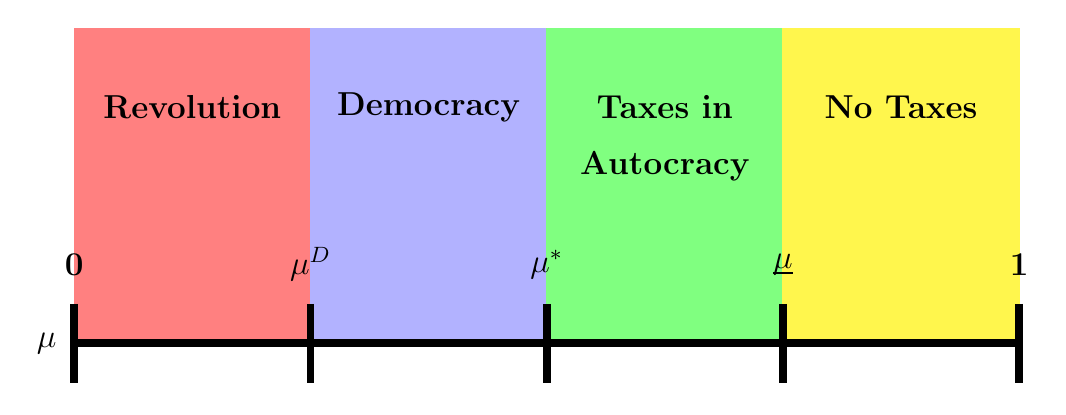
\begin{tikzpicture}	
		\draw[draw = red!50,fill=red!50] (-2,0) -- (1,0) -- (1,4) -- (-2,4) -- (-2,0);
		\draw[draw= blue!30,fill=blue!30] (1,0) -- (4,0) -- (4,4) -- (1,4) -- (1,0);
		\draw[draw=green!50, fill=green!50] (4,0) -- (7,0) -- (7,4) -- (4,4) -- (4,0);
		\draw[draw= yellow!70,fill = yellow!70] (7,0) -- (10,0) -- (10,4) -- (7,4) -- (7,0);
		\node[very thick,align=center,black] (r4) at (4,1)  {\large{$\mu^{*}$}};
		\draw[line width = 1mm] (4,.5) -- (4,-.5);
		\node[very thick,align=center,black] (r4) at (7,1)  {\large{$\mathbf{\underbar{\ensuremath{\mu}}}$}};
		\draw[line width = 1mm] (7,.5) -- (7,-.5);
		\node[very thick,align=center,black] (r4) at (1,1)  {\large{$\mu^{D}$}};
		\draw[line width = 1mm] (1,.5) -- (1,-.5);
		\node[very thick,align=center,black] (r4) at (5.5,3)  {\large{\bf Taxes in}};
		\node[very thick,align=center,black] (r4) at (5.5,2.25)  {\large{\bf Autocracy}};
		\node[very thick,align=center,black] (r4) at (8.5,3)  {\large{\bf No Taxes}};
		\node[very thick,align=center,black] (r4) at (2.5,3)  {\large{\bf Democracy}};
		\node[very thick,align=center,black] (r4) at (-0.5,3)  {\large{\bf Revolution}};
		\draw[line width = 1mm] (-2,0) -- (10,0);
		\draw[line width = 1mm] (-2,.5) -- (-2,-.5);
		\draw[line width = 1mm] (10,.5) -- (10,-.5);
		\node[very thick,align=center,black] (r4) at (-2.35,0) {\large{$\mu$}};
		\node[very thick,align=center,black] (r4) at (-2,1) {\large{\bf 0}};
		\node[very thick,align=center,black] (r4) at (10,1) {\large{\bf 1}};
	\end{tikzpicture}	
	\end{center}
\end{figure}

\subsection{Asset pricing algebra}\label{section:ap4state}

The solution for the pricing kernel revolves around the growth rate of the consumption of the Elites. This can be decomposed as
\begin{equation}
\frac{C_{t+1}^r}{C_{t}^r} \equiv \bigg(\frac{Y_{t+1}}{Y_{t}}\bigg)\left(\frac{c_{t+1}^{r}}{c_{t}^{r}}\right)
\end{equation}
where $c_{t+1}$ is consumption scaled by aggregate income. The growth rate of scaled consumption is given by
\begin{equation}
\frac{c_{t+1}^{r}}{c_{t}^{r}}\equiv \begin{cases} 
Z & \textrm{if }\phi_{t}=1;\phi_{t-1}=0 \\
1 & \textrm{otherwise}
\end{cases} 
\end{equation}
where $Z<1$ represents the penalty the Elites face to their consumption upon a successful transition to democracy. This can take on two values, given by
\begin{equation}
Z \equiv \begin{cases} 
 Z_H = \frac{\hat{y}^{r} (\tau^{pH*},\theta^{DH},\nu^{DH})}{\hat{y}^{r} (\tau_t,\theta^{A},\nu^A)}. & \textrm{with probability }q \\
 Z_L = \frac{\hat{y}^{r} (\tau^{pL*},\theta^{DL},\nu^{DL})}{\hat{y}^{r} (\tau_t,\theta^{A},\nu^A)}. & \textrm{with probability } 1-q \\
\end{cases} 
\end{equation}
Under Epstein-Zin utility, the stochastic discount factor of the Elites is
\[
M_{t+1}=\beta^{\alpha}\bigg(\frac{C_{t+1}^r}{C_{t}^r}\bigg)^{-\frac{\alpha}{\psi}}R_{W,t+1}^{(\alpha-1)}
\]
where $\alpha \equiv \frac{1-\gamma}{1-\frac{1}{\psi}}$. The return on wealth can be written as
\begin{equation}
R_{W,t+1} = \bigg(\frac{\kappa_{t+1}}{\kappa_t - 1}\bigg)\bigg(\frac{C_{t+1}^r}{C_{t}^r}\bigg)
\end{equation}
where $\kappa \equiv W/C$ is the cum-dividend wealth-consumption ratio. Conjecture that $\kappa$ is constant in each state of $\mu$. This means that the solution is given by the solution to the system of equations
\begin{equation}
\kappa(\mu^j)=1+\beta e^{(1-\frac{1}{\psi})\bar{y}+\frac{1}{2}(1-\gamma)(1-\frac{1}{\psi})\sigma_y^2} \bigg[\mathbf{e}_j^\prime \mathbf{P}\boldsymbol\kappa^{\alpha}\bigg]^{\frac{1}{\alpha}}
\end{equation}
in states 1 and 2, where
\begin{equation}
\boldsymbol{\kappa}^{\alpha}\equiv\begin{pmatrix}\kappa(\mu^{1})^{\alpha}\\
\kappa(\mu^{2})^{\alpha}\\
\kappa(\mu^{3})^{\alpha}(qZ_H^{1-\gamma} + (1-q)Z_L^{1-\gamma})
\end{pmatrix}.
\end{equation}
In state 3, the wealth-consumption ratio is
$$
\kappa(\mu^{3})=\frac{1}{1-\beta e^{(1-\frac{1}{\psi})\bar{y}+\frac{1}{2}(1-\gamma)(1-\frac{1}{\psi})\sigma_y^{2}}}.
$$
This system of equations can be solved numerically.

The riskfree rate, similar to the wealth-consumption ratio, varies only with the state of $\mu$ and is given by
\begin{align*}
R_{f}(\mu_t) = \E\bigg[\beta^{\alpha}\bigg(\frac{C^r_{t+1}}{C^r_{t}}\bigg)^{-\gamma}\bigg(\frac{\kappa(\mu_{t+1})}{\kappa(\mu_{t})-1}\bigg)^{\alpha-1}\bigg]^{-1}.
\end{align*}
This once again yields a system of 3 equations for the riskfree rate, which are characterized by
\begin{equation}
R_{f}(\mu^{j})= \beta^{-\alpha}e^{\gamma\bar{y} -\frac{1}{2}\gamma^2 \sigma_y^2}\left(\kappa(\mu^{j})-1\right)^{\alpha-1}\bigg[\mathbf{e}_j^\prime \mathbf{P}\boldsymbol\kappa^{\alpha-1}\bigg]^{-1}
\end{equation}
in states 1 and 2, where
\begin{equation}
\boldsymbol{\kappa}^{\alpha-1}\equiv\begin{pmatrix}\kappa(\mu^{1})^{\alpha-1}\\
\kappa(\mu^{2})^{\alpha-1}\\
\kappa(\mu^{3})^{\alpha-1}(qZ_H^{-\gamma} + (1-q)Z_L^{-\gamma})
\end{pmatrix}.
\end{equation}
This riskfree rate in the 3rd state is given by
\begin{equation*}
R_{f}(\mu^3)= \beta^{-1}e^{\frac{1}{\psi}\bar{y} - \frac{1}{2}(\gamma-\frac{1}{\psi}(1-\gamma))\sigma_y^2}.
\end{equation*}

Recall that the dividend claim follows:
\begin{equation*}
\frac{D_{t+1}}{D_{t}} \equiv \bigg(\frac{Y_{t+1}}{Y_{t}}\bigg)^{\Upsilon}\chi^D_{t+1}.
\end{equation*}
This implies that the price-dividend ratio can be expressed as
\begin{equation}
1=\mathbb{E}_t\bigg[\beta^{\alpha}\bigg(\frac{C_{t+1}}{C_{t}}\bigg)^{\Upsilon-\gamma}\bigg(\frac{\kappa_{t+1}}{\kappa_t - 1}\bigg)^{(\alpha-1)} \chi^{-\gamma}_{t+1}\chi^D_{t+1} \bigg(\frac{pd_{t+1}+1}{pd_{t}}\bigg)\bigg]
\end{equation}
where $pd$ is the ex-dividend price-dividend ratio. In democracy, the price-dividend ratio is given by
\begin{equation}
pd(D) = \beta e^{(\Upsilon-\frac{1}{\psi})\bar{y}+\frac{1}{2}((\Upsilon-\gamma)^2 + (1-\gamma)(\gamma-\frac{1}{\psi}))\sigma_y^{2}} \bigg(pd_{t+1}+1\bigg)
\end{equation}
which implies that 
\begin{equation}
pd(D) = \frac{\beta e^{(\Upsilon-\frac{1}{\psi})\bar{y}+\frac{1}{2}((\Upsilon-\gamma)^2 + (1-\gamma)(\gamma-\frac{1}{\psi}))\sigma_y^{2}}}{1-\beta e^{(\Upsilon-\frac{1}{\psi})\bar{y}+\frac{1}{2}((\Upsilon-\gamma)^2 + (1-\gamma)(\gamma-\frac{1}{\psi}))\sigma_y^{2}}}.
\end{equation}

\subsection{Gradual redistribution}\label{section:gradual_redist}

In actual democratizations redistribution happens gradually. However, in the model in the main text, redistribution happens all at once upon the conclusion of a successful transition to democracy. This appendix section reformulates the model to allow for more gradual redistribution. Here, we have Elite consumption following the same as in Equation (\ref{eq:elite_consumption}) by $\chi$ is now equal to
\begin{equation}
\chi_{t+1} \equiv \begin{cases} 
e^{- \bar{y}^r} & \textrm{if }\phi_{t}=1 \\
1 & \textrm{otherwise}
\end{cases}.
\end{equation}
Here, $\chi$ represents a permanent reduction in the growth rate of elite consumption. As in the previous model, this can take on two value:
\begin{equation}
\bar{y}^r \equiv \begin{cases} 
 \bar{y}^r_H & \textrm{with probability }q \\
 \bar{y}^r_L & \textrm{with probability }1-q \\
\end{cases} 
\end{equation}
where $\bar{y}^r_H < \bar{y}^r_L$. Just as in Appendix~\ref{section:ap4state} above, the stochastic discount factor of the Elites is
\[
M_{t+1}=\beta^{\alpha}\bigg(\frac{C_{t+1}^r}{C_{t}^r}\bigg)^{-\frac{\alpha}{\psi}}R_{W,t+1}^{(\alpha-1)}
\]
where $\alpha \equiv \frac{1-\gamma}{1-\frac{1}{\psi}}$. The return on wealth can be written as
\begin{equation}
R_{W,t+1} = \bigg(\frac{\kappa_{t+1}}{\kappa_t - 1}\bigg)\bigg(\frac{C_{t+1}^r}{C_{t}^r}\bigg)
\end{equation}
where $\kappa \equiv W/C$ is the cum-dividend wealth-consumption ratio. Conjecture that $\kappa$ is constant in each state of $\mu$.  This means that the solution is given by the solution to the system of equations
\begin{equation}
\kappa(\mu^j)=1+\beta e^{(1-\frac{1}{\psi})\bar{y}+\frac{1}{2}(1-\gamma)(1-\frac{1}{\psi})\sigma_y^2} \bigg[\mathbf{e}_j^\prime \mathbf{P}\boldsymbol\kappa^{\alpha}\bigg]^{\frac{1}{\alpha}}
\end{equation}
in states 1 and 2, where
\begin{equation}
\boldsymbol{\kappa}^{\alpha}\equiv\begin{pmatrix}\kappa(\mu^{1})^{\alpha}\\
\kappa(\mu^{2})^{\alpha}\\
q \kappa_H(\mu^{3})^{\alpha} e^{-(1-\gamma)\bar{y}^r_H} + (1-q) \kappa_L(\mu^{3})^{\alpha} e^{-(1-\gamma)\bar{y}^r_L} 
\end{pmatrix}.
\end{equation}
In state 3, the wealth-consumption ratio is
$$
\kappa_k(\mu^{3})=\frac{1}{1-\beta e^{(1-\frac{1}{\psi})(\bar{y}-\bar{y}^r_k)+\frac{1}{2}(1-\gamma)(1-\frac{1}{\psi})\sigma_y^{2}}}
$$
with $k\in\{H,L\}$. This system of equations can be solved numerically.

For simplicity, I assume that the dividend claim is purely a levered claim to elite consumption
\begin{equation*}
\frac{D_{t+1}}{D_{t}} \equiv \bigg(\frac{C^r_{t+1}}{C^r_{t}}\bigg)^{\Upsilon}.
\end{equation*}
This implies that the price-dividend ratio can be expressed as
\begin{equation}
1=\mathbb{E}_t\bigg[\beta^{\alpha}\bigg(\frac{C_{t+1}}{C_{t}}\bigg)^{\Upsilon-\gamma}\bigg(\frac{\kappa_{t+1}}{\kappa_t - 1}\bigg)^{(\alpha-1)} \chi^{\Upsilon-\gamma}_{t+1} \bigg(\frac{pd_{t+1}+1}{pd_{t}}\bigg)\bigg]
\end{equation}
where $pd$ is the ex-dividend price-dividend ratio. In democracy, the price-dividend ratio is given by
\begin{equation}
pd_k(D) = \frac{\beta e^{(\Upsilon-\frac{1}{\psi})(\bar{y}-\bar{y}^r_k)+\frac{1}{2}((\Upsilon-\gamma)^2 + (1-\gamma)(\gamma-\frac{1}{\psi}))\sigma_y^{2}}}{1-\beta e^{(\Upsilon-\frac{1}{\psi})(\bar{y}-\bar{y}^r_k)+\frac{1}{2}((\Upsilon-\gamma)^2 + (1-\gamma)(\gamma-\frac{1}{\psi}))\sigma_y^{2}}}
\end{equation}
where again $k\in\{H,L\}$. This can also be solved numerically.


\section{Case studies of democratization}\label{section:case_studies}

\subsection{Sweden, 1917--1924}\label{section:SWEDEN}

The fall of the monarchy in Sweden offers an excellent example of a democratization associated with a large stock market response combined with subsequent redistribution. Relative to its Scandinavian neighbors, Sweden was slow to democratize. This changed in 1917. The year began with a conservative government in power. By autumn, however, this government had been forced from office due to ``food riots and the unreliability of the army'' \citep{Luebbert1991}. Worker and soldier unrest continued into 1918 and by October the decisive democratic breakthrough had occurred.  This victory brought with it a coalition Liberal-Social Democrat government from 1918--1920 which instituted several pro-labor policies through strengthening the already strong trade unions and instituting the 8 hour work day \citep{Bengtsson2014}. Universal suffrage was also established during this time, with the first elections under universal suffrage taking place between September 10th and 26th in 1921. V-Dem's Electoral Democracy Index tracks this progress well, as shown in Figure~\ref{fig:SWEDEN}, showing an initial increase in 1918 and final increase in 1922 as the newly elected government takes power.

While these policy changes did not immediately bring forth the famed Swedish welfare state---that would come about during and after the Great Depression---they did alter the bargaining power between labor and capital tremendously. For example, \cite{Bengtsson2014} finds a structural break in the capital share of income in 1920, with the capital share going from a high of 40\% in 1916 down to 20\% just after 1920. Moreover, this effect seemed to permanent; from 1920--2000, it would not reach above 30\% again.

\begin{figure}[t!]
    \captionsetup{width=1\linewidth}
	\caption{\textbf{Electoral Democracy Index and dividend yield, Sweden 1917--1924}}
	\renewcommand{\baselinestretch}{1}
    \captionsetup{singlelinecheck=off}
	\label{fig:SWEDEN}
	\footnotesize 
	\vspace{-.75cm}
    \begin{center}
		\includegraphics[width=1\textwidth]{figure_F12_sweden_case_study.pdf}
	\end{center}
\end{figure}
Additional support for a nearly immediate reduction in inequality comes from examining top income shares. While exact numbers on how much inequality declined after the democratization are somewhat contested, recent research by \cite*{Bengtsson2021} on a random sample of tax returns in Stockholm indicate that the Gini coefficient fell by at much as 20 percentage points and the top 10\% share of income by 15 percentage points from 1920 to 1940. For comparison, the World Inequality Database (WID) reports that the top 10\% share in the United Kingdom and United States remained flat over this period, and in France only declined by 5 percentage points.  Similarly, the WID reports that the top 1\% income share in Sweden fell by 8 percentage points, compared to 5 percentage points in the UK and France from 1919--1941. It remained flat in the U.S. over this period. \cite{Bengtsson2019} also notes the discontinuity in Swedish income inequality post-democratization.

Finally, the Swedish democratization brought with it large increases in the dividend yield as shown in Figure~\ref{fig:SWEDEN}. The dividend yield began to rise in 1917 with the labor unrest and calls for increased political rights. In the year of the democratic breakthrough, the dividend yield rose further with the onset of the democratic breakthrough. From 1917--1920, the outcome of the democratization remained highly uncertain. However, as 1920 came to an end, the shift of power toward the left became complete, and brought with it large declines to inequality. With this uncertainty resolved, the dividend yield began to fall to its pre-democratization levels.

\subsection{France, 1847--1848}\label{section:FRANCE}

The establishing of the Second French Republic in the wake of the revolution of 1848 presents an excellent example of a failed democratization.  The movement toward 1848 began in 1847 with the beginning of the Reformist ``banquets'' at which toasts were drunk to the \textit{R\'{e}publique fran\c{c}aise} \citep{Marx1850}. This \textit{Campagne des banquets} was constructed to circumvent the restriction on political gatherings levied by the monarchy. While mostly liberal in nature, these banquets were also attended by reformists of all kinds; for example, a young Friedrich Engels attended some of these banquets starting in October 1847. King Louis Philippe allowed for these Reformist meetings to continue, resulting in an increase in free expression in the Electoral Democracy Index, as shown in Figure~\ref{fig:FRANCE}.  

As the banquets became more revolutionary in nature,  however, the Prime Minister of France, Fran\c{c}ois Guizot, outlawed them in January, 1848. Despite this ban, the gatherings continued. Things came to a head on February 22nd, when the French government banned the banquets for the second time, leading the organizing committee to cancel the events. Workers and students, however, had been mobilizing prior to the ban, and they did not plan to cancel their demonstration. It was with these demonstrations that a second ``Three Glorious Days'' began, leading to the ousting of King Louis Philippe on February 24th.

Shortly after the abdication of King Louis Philippe, the Second French Republic was declared. However, the democratic progress was short lived. Infighting in the proto-socialist groups made them politically ineffectual and ultimately led to the election of Louis Napoleon Bonaparte in the election of 1848. Bonaparte, a man viewed as the arch-ally to the \textit{bourgeoisie} by Marx, ultimately fully reversed the democratic progress in his famed 1851 \textit{coup d'\'{e}tat}, which established the Second French Empire.

Also shown in Table~\ref{fig:FRANCE} is the movement in the dividend yield across the failed democratization. Dividend yields spike in 1848 with the initial unrest and fall of the monarch. They then drop after the election of Louis Napoleon, but remain elevated until 1851, and the establishment of the Second Empire. In 1851 and 1852, stock prices rose 27\% and 53\%, respectively, signaling both the end of the episode, and investors' satisfaction with the 1851 coup.

\begin{figure}[t!]
    \captionsetup{width=1\linewidth}
	\caption{\textbf{Electoral Democracy Index and dividend yield, France 1847--1848}}
	\renewcommand{\baselinestretch}{1}
    \captionsetup{singlelinecheck=off}
	\label{fig:FRANCE}
	\footnotesize 
	\vspace{-.75cm}
    \begin{center}
		\includegraphics[width=1\textwidth]{figure_F13_france_case_study.pdf}
	\end{center}
\end{figure}


\section{List of democratizations}

Table~\ref{table:fastDem} shows the list of democratizations used in the asset pricing results.

\newpage
\footnotesize
\begin{longtable}{lcc}
	\caption{\textbf{List of ERT democratizations used in dividend yield results}}  \\ 
	\hline 
	\toprule 
	\textbf{Country} & \textbf{Democratizations} & \textbf{Major Events}  \\ \hline
	\midrule 
	\endfirsthead 
	\toprule 
	\textbf{Country} & \textbf{Democratizations} & \textbf{Major Events}  \\ 
	\midrule 
	\endhead 
	\midrule 
	\multicolumn{3}{c}{\footnotesize(Continued on next page)} 
	\endfoot 
	\bottomrule 
	\endlastfoot 
	\label{table:fastDem}
		Argentina  &  \parbox[t][][t]{2cm}{\centering1916--1926} & \parbox[t][][t]{10cm}{ 1916: First Presidential Election with universal male sufferage \\ 1921: Passage of Labor Codes \\ 1922: Successful transition of power to Alvear Administration} \vspace*{.15cm} \\ \hline
Argentina  &  \parbox[t][][t]{2cm}{\centering1932--1940} & \parbox[t][][t]{10cm}{ 1932: Removal of Jose Felix Uriburu after turn toward fascism \\ 1932: (Fraudulent) election after coup \\ 1933: Survival of attempted coups \\ 1937: General strike in support of construction workers \\ 1938: Ortiz administration attempts to curtail electoral fraud} \vspace*{.15cm} \\ \hline
Argentina  &  \parbox[t][][t]{2cm}{\centering1946--1948} & \parbox[t][][t]{10cm}{ 1946: Presidential election which Peron won in a landslide \\ 1947: Suffrage extended to women \\ 1948: Successful legislative election} \vspace*{.15cm} \\ \hline
Argentina  &  \parbox[t][][t]{2cm}{\centering1972--1974} & \parbox[t][][t]{10cm}{ 1972: Peronists begin general strikes and protests \\ 1972: Return of Juan Peron from exile \\ 1973: First elections in 10 years \\ 1973: Juan Peron second presidency \\ 1974: Death of Juan Peron \\ 1974: Beginning of Isabel Peron administration} \vspace*{.15cm} \\ \hline
Australia  &  \parbox[t][][t]{2cm}{\centering1843--1844} & \parbox[t][][t]{10cm}{ 1843: First parlimentary election} \vspace*{.15cm} \\ \hline
Australia  &  \parbox[t][][t]{2cm}{\centering1856--1858} & \parbox[t][][t]{10cm}{ 1856: Beginning of Responsible Government \\ 1856: Eight hour workday introduced \\ 1856: Manhood suffrage introduced \\ 1856: South Australian Constitution \\ 1858: Secret Ballot introduced \\ 1858: Women granted right to divorce} \vspace*{.15cm} \\ \hline
Australia  &  \parbox[t][][t]{2cm}{\centering1901--1904} & \parbox[t][][t]{10cm}{ 1901: Formation of the Australian federation \\ 1901: Commonwealth of Australia proclaimed \\ 1901: Australian Labor Party becomes official federal party \\ 1901: First federal election \\ 1902: Women receive right to vote \\ 1903: High Court of Australia established \\ 1903: Women vote in first election \\ 1904: First Labor government} \vspace*{.15cm} \\ \hline
Australia  &  \parbox[t][][t]{2cm}{\centering1918--1923} & \parbox[t][][t]{10cm}{ 1918: Beginning of industrial unrest \\ 1918: End of WWI bring end to conscription of troops \\ 1919: Preferential voting introduced \\ 1921: First Woman elected to parliament \\ 1922: Queensland abolishes upper house} \vspace*{.15cm} \\ \hline
Belgium  &  \parbox[t][][t]{2cm}{\centering1894--1900} & \parbox[t][][t]{10cm}{ 1893: General strike for suffrage \\ 1894: First election under universal manhood sufferage \\ 1894: Beginning of welfare net \\ 1896: Beginning Liberal-Labor alliance \\ 1900: Election of 1900} \vspace*{.15cm} \\ \hline
Belgium  &  \parbox[t][][t]{2cm}{\centering1919--1922} & \parbox[t][][t]{10cm}{ 1919: End of German occupation \\ 1919: Beginning of Labor-Catholic Party coalition \\ 1919: Introduction of graduated income tax \\ 1919: First election with universal single-vote suffrage \\ 1921: General election} \vspace*{.15cm} \\ \hline
Belgium  &  \parbox[t][][t]{2cm}{\centering1944--1950} & \parbox[t][][t]{10cm}{ 1944: End of German occupation \\ 1944: Social Pact between labor party and trade unions \\ 1945: Return of government in exile \\ 1946: General election \\ 1949:  Introduction of women's sufferage \\ 1950: General strike and abdication of King Leopold} \vspace*{.15cm} \\ \hline
Belgium  &  \parbox[t][][t]{2cm}{\centering1961--1965} & \parbox[t][][t]{10cm}{ 1961: ``Strike of the Century'' \\ 1961: Linking of Walloon nationalism with syndicalism \\ 1961: Decolonization of Congo \\ 1965: End of Congo Crisis} \vspace*{.15cm} \\ \hline
Bahrain  &  \parbox[t][][t]{2cm}{\centering2000--2003} & \parbox[t][][t]{10cm}{ 1999: Death of Shaikh Isa bin Salman Al Khalifa \\ 2000: Creation of Supreme Judicial Council \\ 2001: National Action Charter \\ 2002: New constitution \\ 2002: Legislative Election \\ 2002: Women's right to vote} \vspace*{.15cm} \\ \hline
Brazil  &  \parbox[t][][t]{2cm}{\centering1945--1950} & \parbox[t][][t]{10cm}{ 1945: End of the Estado Novo \\ 1945: Beginning of Social Democratic Party dominance \\ 1946: Fifth constitution of Brazil \\ 1947: Legislative election \\ 1950:: General election} \vspace*{.15cm} \\ \hline
Canada  &  \parbox[t][][t]{2cm}{\centering1867} & \parbox[t][][t]{10cm}{ 1867: Creation of the Dominion of Canada} \vspace*{.15cm} \\ \hline
Canada  &  \parbox[t][][t]{2cm}{\centering1920--1938} & \parbox[t][][t]{10cm}{ 1920: Dominion Elections Act \\ 1920: Formation of Progressive Party of Canada \\ 1921: Election of first woman to House of Commons \\ 1922: Full suffrage to black and white women in most provinces \\ 1925: Extension of suffrage in Newfoundland and Labrador \\ 1925: Election with continued Progressive Party success \\ 1926: King-Byng affair} \vspace*{.15cm} \\ \hline
Canada  &  \parbox[t][][t]{2cm}{\centering1942--1954} & \parbox[t][][t]{10cm}{ 1942: A national plebiscite is held on the issue of conscription \\ 1942: Income War Tax Act brings increased labor mobilization \\ 1949: End of Judicial Committee of the Privy Council appeals in Canada \\ } \vspace*{.15cm} \\ \hline
Switzerland  &  \parbox[t][][t]{2cm}{\centering1970--1972} & \parbox[t][][t]{10cm}{ 1971: First National Election with Women Voting} \vspace*{.15cm} \\ \hline
Denmark  &  \parbox[t][][t]{2cm}{\centering1901--1902} & \parbox[t][][t]{10cm}{ 1901: Introduction of parlimentary sovereignty \\ 1901: Folketing election \\ 1902: Landsting election} \vspace*{.15cm} \\ \hline
Denmark  &  \parbox[t][][t]{2cm}{\centering1916--1920} & \parbox[t][][t]{10cm}{ 1915: Women granted right to vote \\ 1916: Beginning of the Danish welfare state \\ 1918: First elections under women's suffrage \\ 1920: Easter Crisis} \vspace*{.15cm} \\ \hline
Denmark  &  \parbox[t][][t]{2cm}{\centering1945--1948} & \parbox[t][][t]{10cm}{ 1945: End of German Occupation \\ 1945: Folketing and Landsting elections \\ 1945: Beginning of Social Democrat dominance \\ 1946: October Note \\ 1948: Faroe Island given ``home rule''} \vspace*{.15cm} \\ \hline
Spain  &  \parbox[t][][t]{2cm}{\centering1931--1934} & \parbox[t][][t]{10cm}{ 1931: Deposition of King Alfonso XIII \\ 1931: Beginning of Second Spanish Republic \\ 1931: New constitution \\ 1933: General election} \vspace*{.15cm} \\ \hline
Spain  &  \parbox[t][][t]{2cm}{\centering1976--1980} & \parbox[t][][t]{10cm}{ 1975: Death of Francisco Franco \\ 1977: First parliamentary election since 1936 \\ 1978: Approval of 1978 Constitution \\ 1979: First general election under new constitution \\ 1981: Survival of attempted coup} \vspace*{.15cm} \\ \hline
Finland  &  \parbox[t][][t]{2cm}{\centering1917--1921} & \parbox[t][][t]{10cm}{ 1917: Independence from Russia \\ 1918: End of Finnish Civil War \\ 1919: New Constitution enacted \\ 1919: Parliamentary election \\ 1919: Social Democrat victory \\ 1921: Official completion of Finnish Independence} \vspace*{.15cm} \\ \hline
Finland  &  \parbox[t][][t]{2cm}{\centering1945--1946} & \parbox[t][][t]{10cm}{ 1945: End of alliance with Nazi Germany \\ 1945: Parliamentary election \\ 1946: Beginning of Mauno Pekkala administration} \vspace*{.15cm} \\ \hline
Finland  &  \parbox[t][][t]{2cm}{\centering1948--1950} & \parbox[t][][t]{10cm}{ 1948: Parliamentary elections \\ 1948: End of Pekkala administration \\  1949: Kemi strike; rejection of Communism \\ 1950: Labor unrest and threat of general strike \\ 1950: Start of a social reform era and welfare state} \vspace*{.15cm} \\ \hline
France  &  \parbox[t][][t]{2cm}{\centering1847--1848} & \parbox[t][][t]{10cm}{ 1847: Beginning of the Reform Movement and the banquets \\ 1848: July Monarchy Ends \\ 1848: Founding of Second French Republic \\ 1848: Election of President Louis-Napoleon Bonaparte} \vspace*{.15cm} \\ \hline
France  &  \parbox[t][][t]{2cm}{\centering1966} & \parbox[t][][t]{10cm}{ 1966: Founding of Democratic Centre party \\ 1966: Beginning of student movement toward May 68} \vspace*{.15cm} \\ \hline
Hong Kong  &  \parbox[t][][t]{2cm}{\centering1989--1992} & \parbox[t][][t]{10cm}{ 1989: Tienanmen Square Protests \\ 1989: Founding of Hong Kong Alliance in Support of Patriotic Democratic Movements of China \\ 1990: Beijing ratifies Hong Kong's Basic Law \\ 1991: Introduction of directly elected seats in legislature \\ 1992: Governor Chris Patten announces reform package} \vspace*{.15cm} \\ \hline
Indonesia  &  \parbox[t][][t]{2cm}{\centering1945--1957} & \parbox[t][][t]{10cm}{ 1945: Beginning of Indonesian National Revolution \\ 1946: Beginning of Republican government in Jakarta \\ 1949: Independence \\ 1950: Provisional Constitution of 1950 \\ 1951: Founding of Indonesian Communist Party \\ 1955: First parlimentary elections \\ 1957: System of Guided Democracy} \vspace*{.15cm} \\ \hline
Indonesia  &  \parbox[t][][t]{2cm}{\centering1997--2004} & \parbox[t][][t]{10cm}{ 1997: Indonesian legislative election \\ 1998: Student demonstrations begin \\ 1998: Collapse of Suharto regime \\ 1999: First democratic elections \\ 2000: Process of Constitutional reform \\ 2004: Presidential election} \vspace*{.15cm} \\ \hline
India  &  \parbox[t][][t]{2cm}{\centering1950--1957} & \parbox[t][][t]{10cm}{ 1950: Adoption of Constitution of India \\ 1950: First Republic Day \\ 1951: General election \\ 1952: Completion of General election \\ 1957: General election} \vspace*{.15cm} \\ \hline
India  &  \parbox[t][][t]{2cm}{\centering1977--1979} & \parbox[t][][t]{10cm}{ 1977: End of emergency powers \\ 1977: Founding of Congress for Democracy \\ 1977: General Elections; first loss for the Congress \\ 1978: Appointment of Backward Classes Commission \\ 1979: Fall of Janata Party} \vspace*{.15cm} \\ \hline
Kenya  &  \parbox[t][][t]{2cm}{\centering1990--2003} & \parbox[t][][t]{10cm}{ 1990: Increased congressional pressure for reform \\ 1991: Founding of Forum for the Restoration of Democracy (FORD-Kenya) \\ 1991: Repeal of one party amendment \\ 1992: General election \\ 1993: Successful transition to multiparty rule \\ 2003: FORD-Kenya election victory} \vspace*{.15cm} \\ \hline
South Korea  &  \parbox[t][][t]{2cm}{\centering1981--2000} & \parbox[t][][t]{10cm}{ 1980: Gwangju Uprising \\ 1981: Founding of Fifth Republic of Korea \\ 1987: June Democracy Movement \\ 1987: First democratic elections \\ 1988: Founding of Sixth Republic of Korea \\ 1988: New Constitution \\ 1993: Reforms clamping down on corruption \\ 1998: Inauguration of Kim Dae-jung \\ 1998: First peaceful tranfer of power between parties} \vspace*{.15cm} \\ \hline
South Korea  &  \parbox[t][][t]{2cm}{\centering2017--2018} & \parbox[t][][t]{10cm}{ 2017: Park Geun-hye's removal from office \\ 2017: President Moon Jae-in elected \\ 2018: Park sentenced to 25 years in prison for bribery, coercion, and abuse of power} \vspace*{.15cm} \\ \hline
Sri Lanka  &  \parbox[t][][t]{2cm}{\centering1947--1949} & \parbox[t][][t]{10cm}{ 1947: First elected parliamentary government \\ 1947: New republican constitution replaced the Soulbury Constitution \\ 1948: Discriminatory legislation passed \\ 1949: Tamil congress splits; Federal Party is formed} \vspace*{.15cm} \\ \hline
Sri Lanka  &  \parbox[t][][t]{2cm}{\centering2015--2017} & \parbox[t][][t]{10cm}{ 2015: Presidential elections \\ 2015: Vote for Mahinda Rajapaksa; does not belong to established political party \\ 2015: Agenda to reverse near autocratic actions of last decade \\ 2016: New president lifts ban on Tamil} \vspace*{.15cm} \\ \hline
Malaysia  &  \parbox[t][][t]{2cm}{\centering2018} & \parbox[t][][t]{10cm}{ 2018: Election of the Pakatan Harapan \\ 2018: End of 60 year political reign by United Malays National Organisation \\ 2018: Malay rights groups lead anti-ICERD rally reversing Mahathir's decision to ratify ICERD \\ 2019: Partnership between UNMO and PAS is formalized} \vspace*{.15cm} \\ \hline
Namibia  &  \parbox[t][][t]{2cm}{\centering2013--2016} & \parbox[t][][t]{10cm}{ 2013: Push for gender equality \\ 2014: Election with peaceful transfer of power \\ 2014: Surveys indicate more citizens support democracy \\ 2015: Local and regional elections held with electronic voting \\ 2016: SWAPO power checked by High Court} \vspace*{.15cm} \\ \hline
Nigeria  &  \parbox[t][][t]{2cm}{\centering1976--1980} & \parbox[t][][t]{10cm}{ 1976: Commander in Chief Muhammed killed in abortive coup \\ 1976: General Olusegun Obasanjo, takes over \\ 1976: Minorities vote for new president, Alhaji Shehu Shagari \\ 1978: Obasanjo lifts ban on political parties} \vspace*{.15cm} \\ \hline
Nigeria  &  \parbox[t][][t]{2cm}{\centering2010--2016} & \parbox[t][][t]{10cm}{ 2010: Death of President Umaru Yar'Adua \\ 2011: Election of 2011 (most transparent since 1999)  \\ 2015: Even more transparent general election \\ 2015: Successful transition of power to Muhammadu Buhari} \vspace*{.15cm} \\ \hline
Netherlands  &  \parbox[t][][t]{2cm}{\centering1917--1923} & \parbox[t][][t]{10cm}{ 1917: Universal manhood suffrage implemented \\ 1917: Women allowed to be elected, but not vote \\ 1918: Unsuccessful socialist revolution in November \\ 1919: Full suffrage granted to women \\ 1920: Netherlands joins League of Nations} \vspace*{.15cm} \\ \hline
Netherlands  &  \parbox[t][][t]{2cm}{\centering1945--1980} & \parbox[t][][t]{10cm}{ 1945: End of German occupation \\ 1946: Liberal State Party becomes Freedom Party \\ 1946: Freeminded Democratic League joins Labor Party \\ 1948: People's Party for Freedom and Democracy formed \\ 1966: Democrats 66 formed} \vspace*{.15cm} \\ \hline
Norway  &  \parbox[t][][t]{2cm}{\centering1906--1910} & \parbox[t][][t]{10cm}{ 1906: First parliamentary elections since the end of Union with Sweden \\ 1907: Legislature allows women limited suffrage and ability to hold office \\ 1909: Sorting passes Concessions Laws following much debate and split in Venstre} \vspace*{.15cm} \\ \hline
Norway  &  \parbox[t][][t]{2cm}{\centering1914} & \parbox[t][][t]{10cm}{ 1913: Universal suffrage established \\ 1914: First elections with universal suffrage} \vspace*{.15cm} \\ \hline
Norway  &  \parbox[t][][t]{2cm}{\centering1945--1998} & \parbox[t][][t]{10cm}{ 1945: End of German Occupation \\ 1945: Parliamentary election \\ 1945: Labor wins for first time since 1915 \\ 1948: Break between Labor and Communist parties} \vspace*{.15cm} \\ \hline
New Zealand  &  \parbox[t][][t]{2cm}{\centering1889--1897} & \parbox[t][][t]{10cm}{ 1889: Abolition of plural votes for men of property \\ 1890: First political party, Liberal Party, formed \\ 1893: Universal suffrage granted \\ 1894: Act of 1894 gave state power to repurchase land} \vspace*{.15cm} \\ \hline
Pakistan  &  \parbox[t][][t]{2cm}{\centering2002--2017} & \parbox[t][][t]{10cm}{ 2002: Referendum and General Election \\ 2002: Beginning of multi-party politics after 1999 coup \\ 2003: National assembly \\ 2008: General election; end of Musharraf administration \\ 2008: Official end of military rule \\ 2013: General election \\ 2017: Disqualification of Prime Minister Sharif by Supreme Court} \vspace*{.15cm} \\ \hline
Peru  &  \parbox[t][][t]{2cm}{\centering2001--2004} & \parbox[t][][t]{10cm}{ 2001: Elections after fall of Fujimori \\ 2001: Numerous reforms \\ 2002: Regionalization Law \\ 2002: National Accord \\ 2004: Expansion of social safety net} \vspace*{.15cm} \\ \hline
Philippines  &  \parbox[t][][t]{2cm}{\centering2010--2011} & \parbox[t][][t]{10cm}{ 2010: Presidential election \\ 2010: Introduction of electronic vote counting \\ 2010: Aquino administration; politically stable and relatively clean} \vspace*{.15cm} \\ \hline
Portugal  &  \parbox[t][][t]{2cm}{\centering1970--1984} & \parbox[t][][t]{10cm}{ 1969: Transition to Caetono Regime \\ 1969: Legislative election \\ 1974: Carnation Revolution \\ 1975: Elections for constitutional assembly \\ 1975: Communist coup replaced by moderate coup \\ 1976: Adoption of new constitution \\ 1977: Beginning of European integration process \\ 1979: First woman prime minister Maria de Lourdes Pintasilgo \\ 1980:  Legislative election \\ 1983:  Legislative election; Socialist party victory} \vspace*{.15cm} \\ \hline
Sweden  &  \parbox[t][][t]{2cm}{\centering1917--1924} & \parbox[t][][t]{10cm}{ 1917: Fall of conservative government \\ 1918: Introduction of universal sufferage \\ 1918: First Left-Social Democrat coalition government \\ 1921: First election under universal suffrage \\ 1922: Successful transition of power } \vspace*{.15cm} \\ \hline
Sweden  &  \parbox[t][][t]{2cm}{\centering1971--1974} & \parbox[t][][t]{10cm}{ 1971: Abolished upper house of the Riksdag \\ 1974: New constitution; principles of parliamentarianism incorporated \\ 1974: End of compulsory sterilization program} \vspace*{.15cm} \\ \hline
Thailand  &  \parbox[t][][t]{2cm}{\centering1992--1993} & \parbox[t][][t]{10cm}{ 1992: Black May Protests \\ 1992: General Elections after Coup} \vspace*{.15cm} \\ \hline
Thailand  &  \parbox[t][][t]{2cm}{\centering1997--2001} & \parbox[t][][t]{10cm}{ 1997: Enactment of the ``People's Consitution'' \\ 1997: Chuan Leekpai becomes prime minister \\ 1998: Extension of public programs} \vspace*{.15cm} \\ \hline
Thailand  &  \parbox[t][][t]{2cm}{\centering2008--2012} & \parbox[t][][t]{10cm}{ 2008: Elections held after 2006 military coup \\ 2011: General election; Pheu Thai Party wins in landslide} \vspace*{.15cm} \\ \hline
Tunisia  &  \parbox[t][][t]{2cm}{\centering2011--2016} & \parbox[t][][t]{10cm}{ 2011: Jasmine Revolution ousts  Zine El Abidine Ben Ali \\ 2011: Beginning of Arab Spring \\ 2014: Constitution of 2014 \\ 2014: Parliamentary elections} \vspace*{.15cm} \\ \hline
U.S.A.  &  \parbox[t][][t]{2cm}{\centering1893--1903} & \parbox[t][][t]{10cm}{ 1892: Founding of the Populist Party \\ 1893: Start of the Progressive Era \\ 1893: Beginning of the Anti-Saloon League \\ 1897: Organized labor gains steam with Mother Jones at helm \\ 1903: March on Theodore Roosevelt home by Mother Jones} \vspace*{.15cm} \\ \hline
U.S.A.  &  \parbox[t][][t]{2cm}{\centering1920--1932} & \parbox[t][][t]{10cm}{ 1920: Presidential elections; first where women vote \\ 1921: Washington Naval Conference \\ 1922: First woman senator Rebecca Felton \\ 1927: Reduction in Second Ku Klux Klan popularity \\ 1930: Start of social safety net \\ 1932: Election of President Roosevelt and New Deal} \vspace*{.15cm} \\ \hline
U.S.A.  &  \parbox[t][][t]{2cm}{\centering1970--1977} & \parbox[t][][t]{10cm}{ 1970: Post-civil rights era reforms \\ 1971: Voting age moved to 18 \\ 1974: Watergate and resignation of Nixon \\ 1977: Transition to Carter administration} \vspace*{.15cm} \\ \hline
South Africa  &  \parbox[t][][t]{2cm}{\centering1994--2010} & \parbox[t][][t]{10cm}{ 1994: End of South African Apartheid \\ 1994: Election of Nelson Mandela to presidency \\ 1995: Enactment of new constitution \\ 1999: General election \\ 1999: Beginning of Mbeki presidency \\ 2004: General Election \\ 2005: National Party merges with ANC } \vspace*{.15cm} \\ \hline

\end{longtable}

\newpage

\renewcommand{\baselinestretch}{1}\normalsize
\footnotesize
\setlength{\bibsep}{1pt}
\bibliography{Democratization}
\bibliographystyle{aer}


\end{document}
